\chapter{Results} \label{chap:Results}

%The results chapter should simply present the results of applying the methods presented in the method chapter without further ado. This chapter will typically contain many graphs, tables, etc. Sometimes it is natural to discuss the results as they are presented, combining them into a `Results and Discussion' chapter, but more often they are kept separate.\\ 

The following sections presents the results for each attack type, with subsections for the detection threshold levels selected, as defined in section \ref{sec:ExpDef} 
For each attack type defined, a number of attacks specifying various delay levels, specified as a number of samples, are covered.
For each delay level, a number of figures are produced by running the simulation.
A figure showing a combined view of all three components, displaying the delayed and original signals, as well as a signal indicating the actual difference between the two signals.  Three more detailed figures follows, comparing the original and delayed signal to a similarity measure for each of the three PMU output components.

The delay functions defined, delays the input signal by the specified number of samples, in one or more steps.

% delay.step    
% 1.1
% 2.1 2.2 
% 3.1 3.2 3.3
% 4.1 4.2 4.3 4.4
% 5.1 5.2 5.3 5.4 5.5

Comments on the results are included for selected figures, whereas, interpretation of the results are deferred to chapter \ref{chap:Discussions}
%\newcommand{\locateResults}{PMUsim-figures/}

%\renewcommand{\locateResults}{PMUsim-figures/Cont/DelayOf_0}
%\newpage
\section{Square pulse  delay function: Delay of 6}

\begin{figure}[hb]
 %   \includegraphics[trim=2 10 14 4, clip]{figures/v_AllFig-DelayOf_2-Sqaending.png}    
    \includegraphics[width=0.95\textwidth]{\locateResults/AllFig.png}    
    \caption{Square pulse  delay of 6: Combined output}
    \label{fig:PMUsim-Sqa6-allfig}
\end{figure}


     \begin{figure}
 
    \includegraphics[width=\textwidth]{\locateResults/Magnitude.png}    
         %\caption{Magnitude Output}
         \label{fig:PMUsim-Sqa6Mag}
        \caption{Square pulse  delay of 6: Magnitude component output}
 
\end{figure}

     \begin{figure}
 
   \includegraphics[width=\textwidth]{\locateResults/Angle.png}    
          %\caption{Angle Output}
         \label{fig:PMUsim-Sqa6Ang}
        \caption{Square pulse  delay of 6: Angle component output}
 
\end{figure}

     \begin{figure}
 
   \includegraphics[width=\textwidth]{\locateResults/Frequency.png}    
         %\caption{Frequency Output}
         \label{fig:PMUsim-Sqa6Freq}
        \caption{Square pulse  delay of 6: Frequency component output}
 
\end{figure}








\newpage
\begin{figure}[H]
\begin{tabular}{c}
  \fbox{  \includegraphics[width=0.95\textwidth]{PMUsim-figures/DelayOf_0/Zero_vMagnitude.png}} \\ 
   
   \fbox{    \includegraphics[width=0.95\textwidth]{PMUsim-figures/DelayOf_0/Zero_vFrequency.png}} \\ 

   \fbox{     \includegraphics[width=0.95\textwidth]{PMUsim-figures/DelayOf_0/Zero_vAngle.png}}

  \end{tabular}
\label{fig:VoltageZeroDelay}
\caption{Results for Voltage Output for Delay equal to Zero }
\end{figure}


\section{The Delay Level of Zero}
For model verification purposes, the output for the delay level of zero is included.

One could possibly dispute the relevance of including an attack producing a zero delay level, but the simulation is intended to serve two purposes, as previously explained in subsection \ref{subsec:ModelValidation}:

\begin{enumerate}
\item The design of the \textbf{DualPMU}  subsystem, as visualised in figure \ref{fig:DualPMU}, appears to include two instances of \acrlong{pmu}s of the same \acrshort{pmu} implementation, the SimScape Electric \acrshort{pmu} library module, as previously described in subsection \ref{subsec:ModelPMU}.  
\item The delay function, listed in \ref{tab:vDelay}, is presumably correct. Running a simulation with a constant delay level of Zero should produce the same result as for identical \acrfull{pmu}s, showing identical, and indistinguishable \acrshort{pmu} output, as displayed in the resulting figures.
\end{enumerate}

No matter how identical the \acrshort{pmu} implementations of the  \textbf{DualPMU}  subsystem appears to be: If the delay function erroneously introduces a delay, the resulting output of the simulation is unlikely to produce a correct result, 

The reverse argumentation also sounds reasonalbe:

No matter how perfect the delay function might be, if the simulation produces deviating results, erroneously indicating a, possibly random, delay, the \acrshort{pmu} implementations of the  \textbf{DualPMU}  subsystem  is unlikely to be correct. 

\subsubsection{Result for delay Zero:}

\begin{small}
     \tcbox[size=normal, standard jigsaw, opacityback=0, boxrule=0pt,halign=justify]{
     Comment on the figure:}{
          \begin{itemize}
         \item      The delayed signal (blue) overlaps the original signal (red), producing a straight line, colored neither red nor blue.
         \item  The blue Normalised diff signal also overlaps the grey delay function.
          \end{itemize} }
\end{small}





\newpage
\begin{figure}[H]
\begin{tabular}{c}
    \fbox{ \includegraphics[width=0.95\textwidth]{PMUsim-figures/DelayOf_0/Zero_iMagnitude.png}} \\
	
       \fbox{ 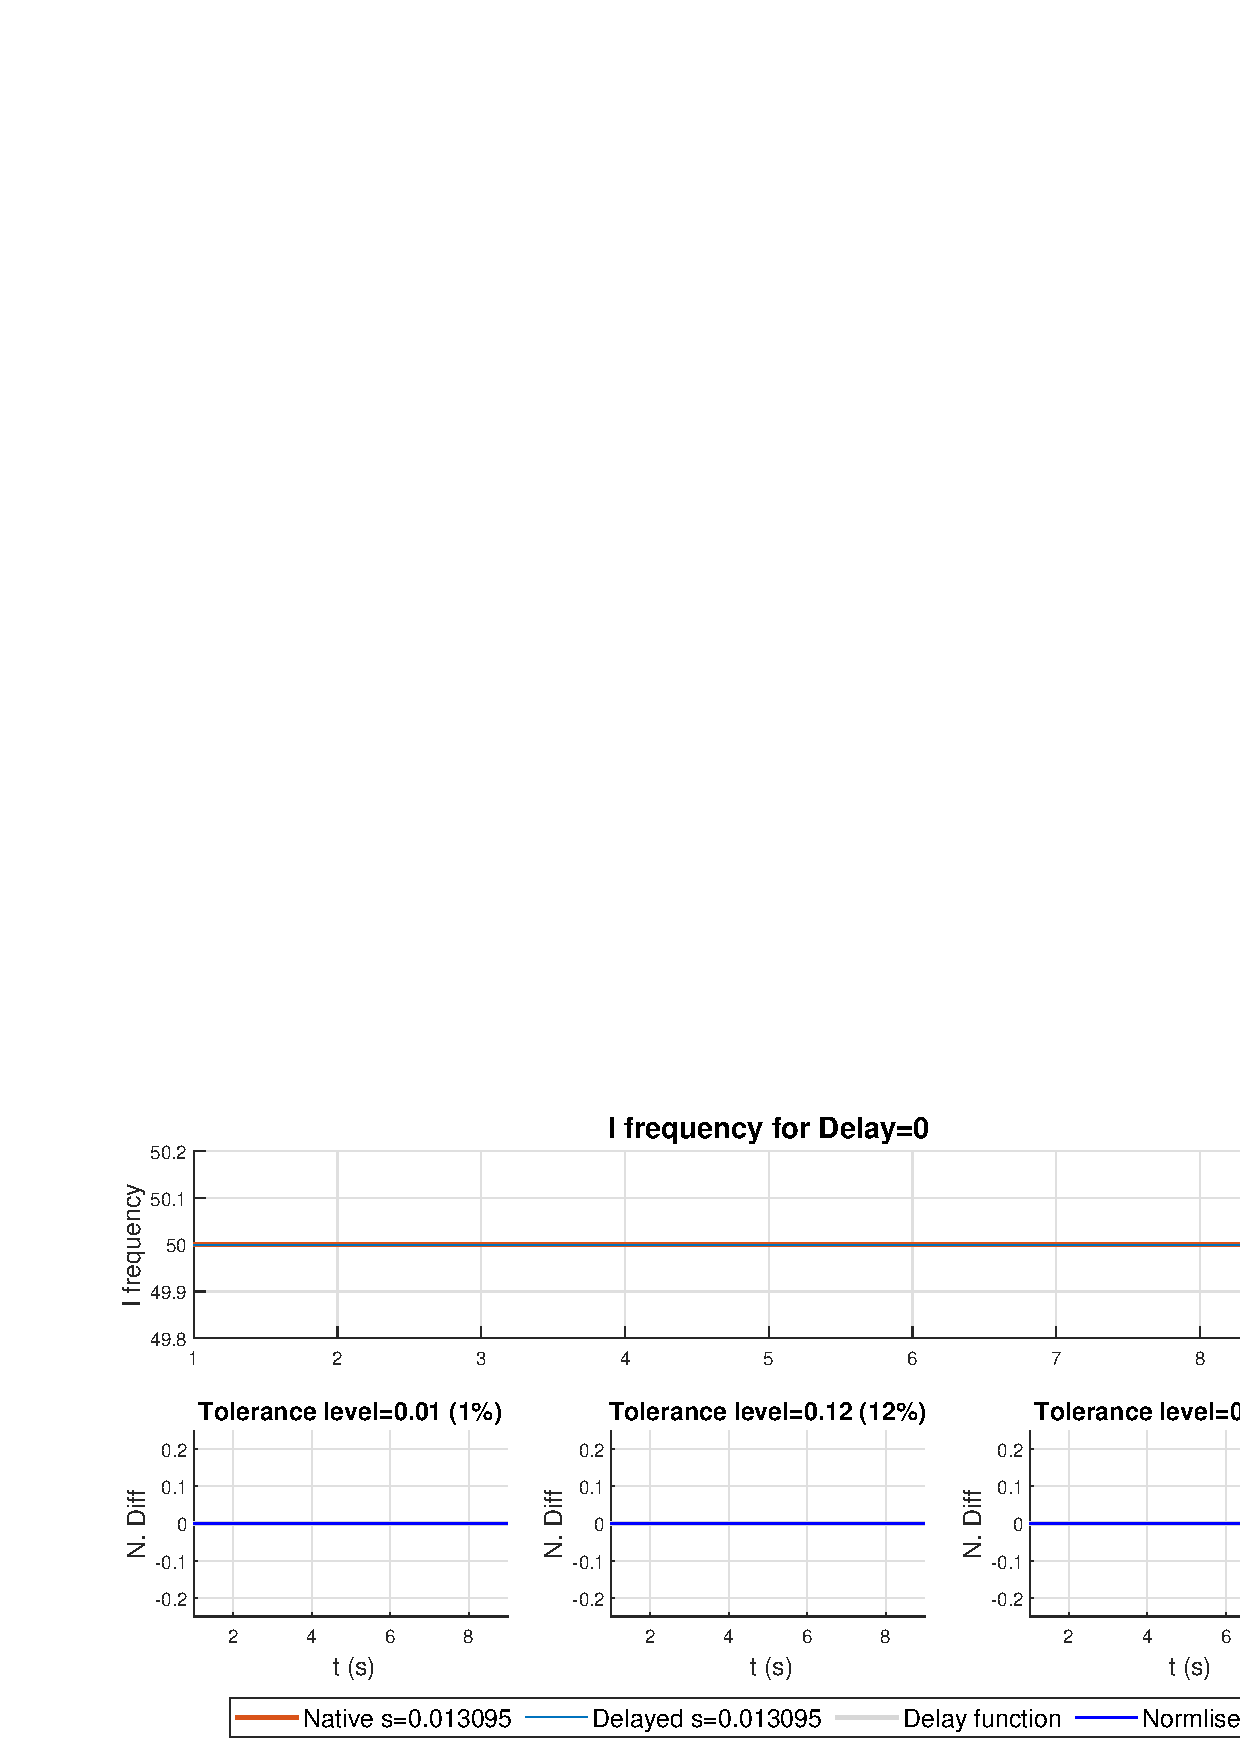
\includegraphics[width=0.95\textwidth]{PMUsim-figures/DelayOf_0/Zero_iFrequency.png}}  \\
	   
   \fbox{  \includegraphics[width=0.95\textwidth]{PMUsim-figures/DelayOf_0/Zero_iAngle.png}} \\ 


 %\caption{Zero Delay Frequency Output (for the Delay Level of Zero)}
  \end{tabular}
\label{fig:ImpedanceZeroDelay}
\caption{Results for Impedance Output for Delay equal to Zero }
\end{figure}









\section{Instant Delay Simulations}
Instant delay simulations are characterised by the delay level instantly raises to the specified level, staying at the same constant level for the entire duration of the simulation, before instantly dropping to zero at the specified attack termination time.
The simulation focuses on:
\begin{itemize}
    \item Observing the situation prior to the attack for the purpose of comparing system state at attack termination with the pre-attack system state.
    \item observing the effect of a prolonged attack of constant level:
    \begin{itemize}
        \item What is the effect of a instant rise of the delay level for various delay levels?
        \item What is the effect of a instant drop of the delay level for various delay levels?
    \end{itemize}
\end{itemize}

On the remaining pages, the figures are available for inspection of the results. Conclusive remarks are available 








\newpage
\begin{figure}[H]
\begin{tabular}{c}
  \fbox{  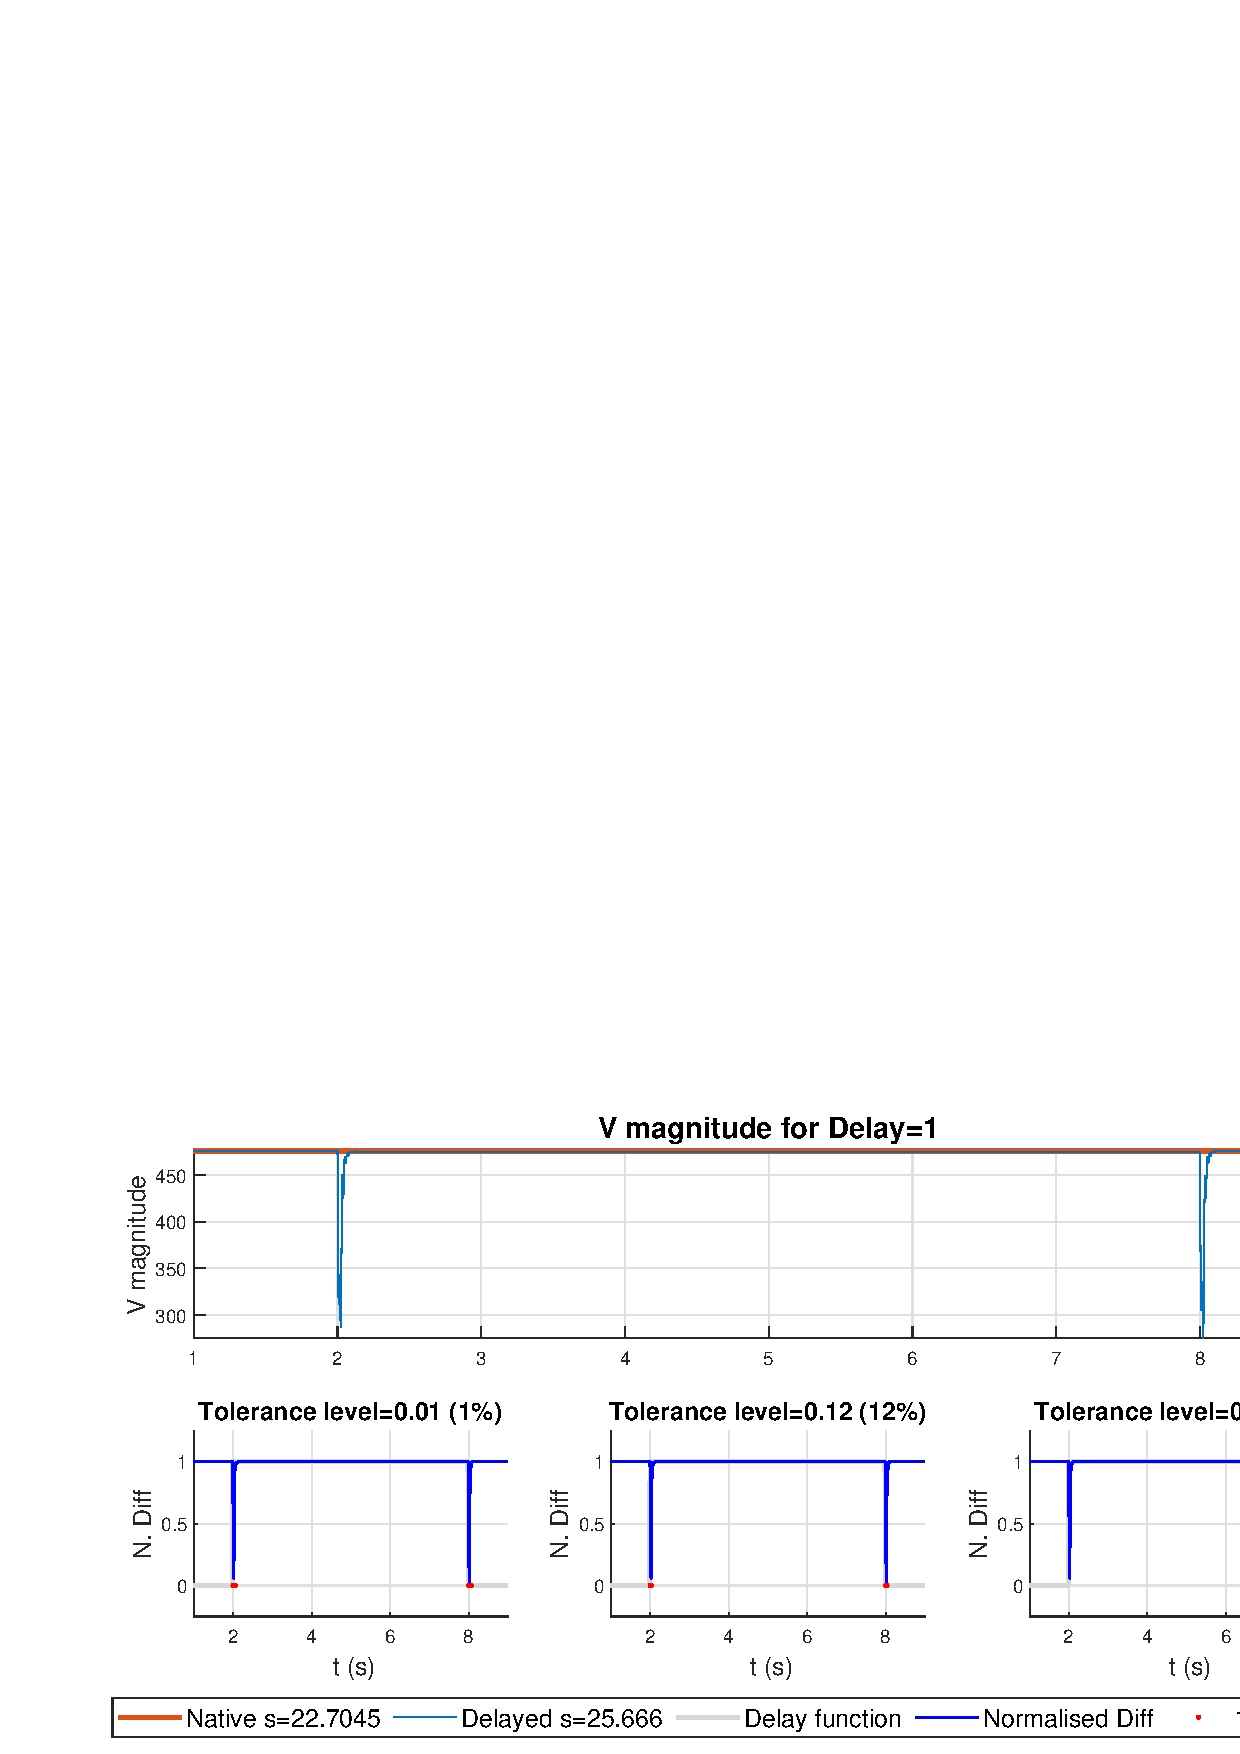
\includegraphics[width=0.95\textwidth]{PMUsim-figures/DelayOf_1/Instant_vMagnitude.png}} \\ 
   \fbox{     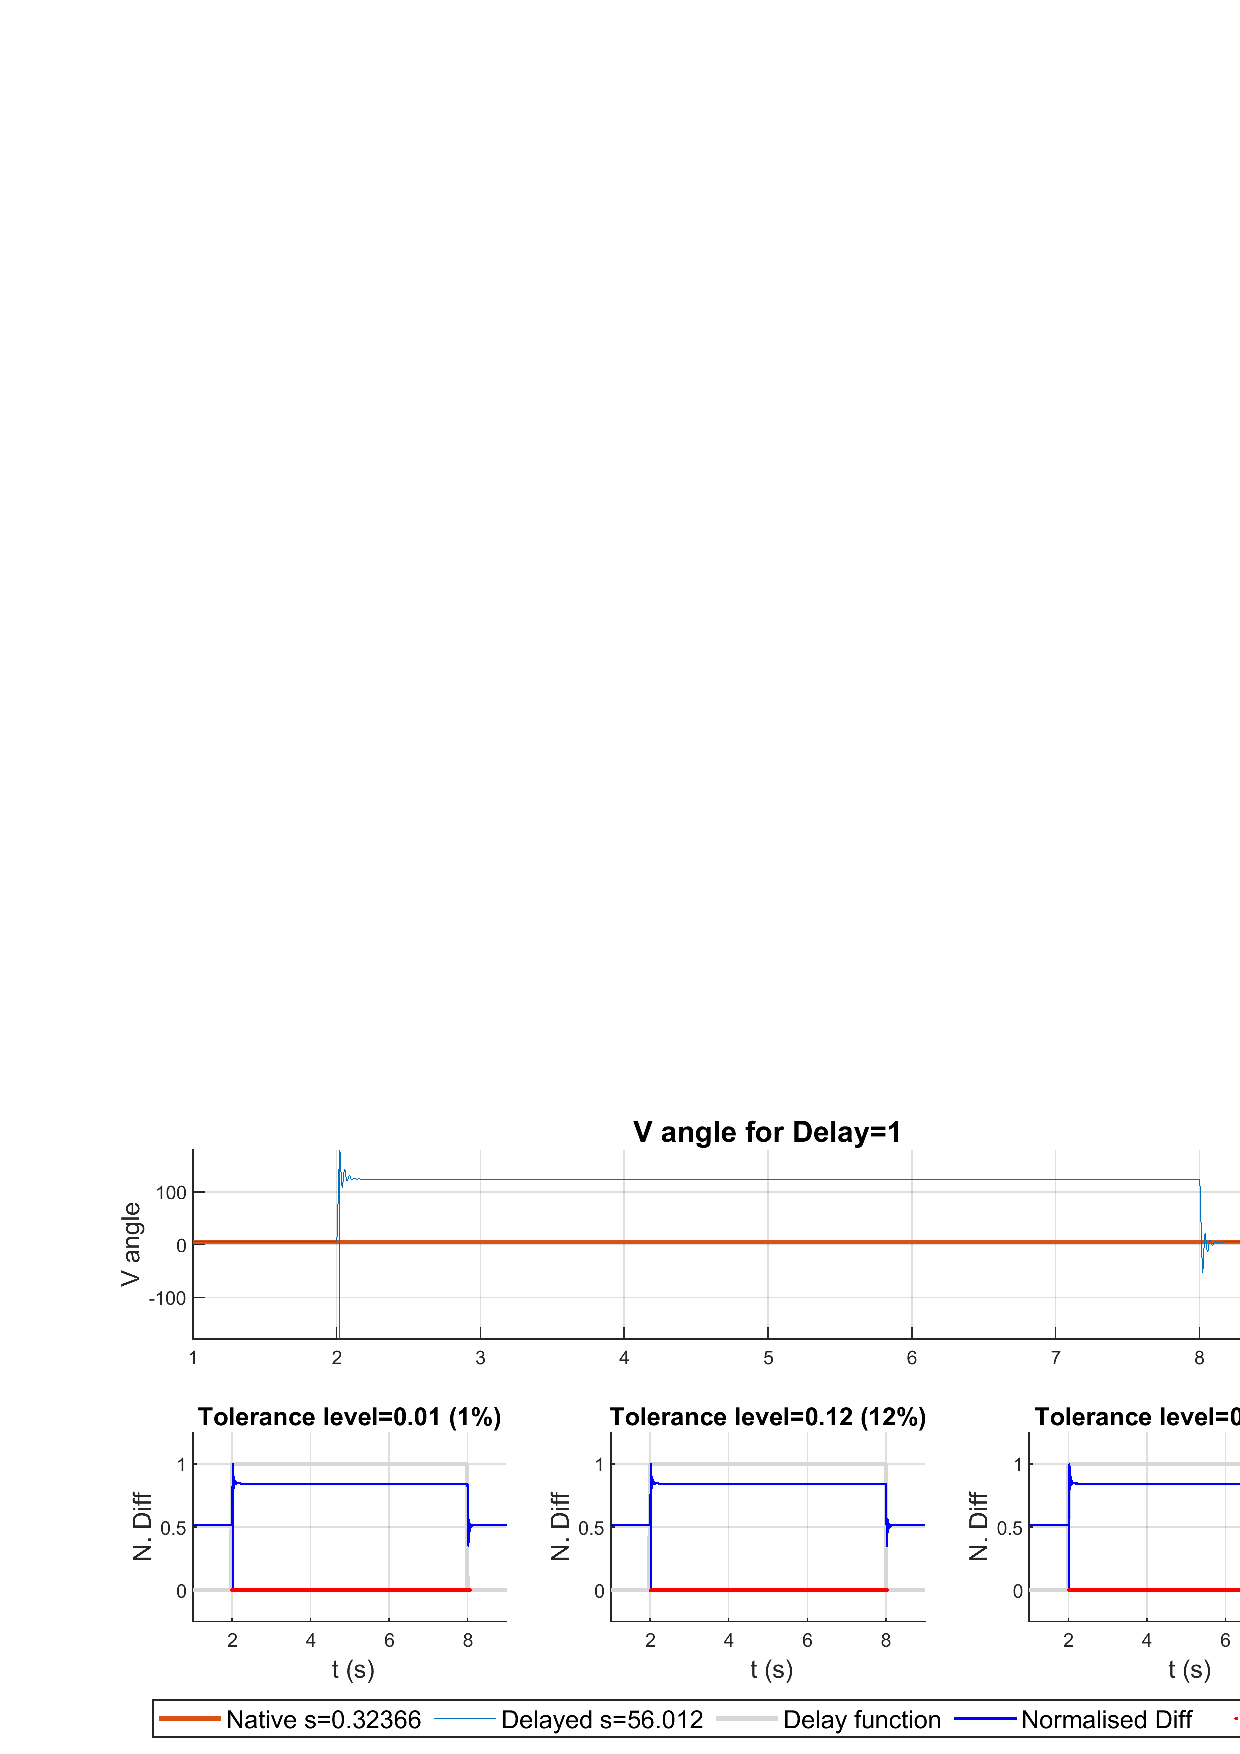
\includegraphics[width=0.95\textwidth]{PMUsim-figures/DelayOf_1/Instant_vAngle.png}} \\   
   \fbox{    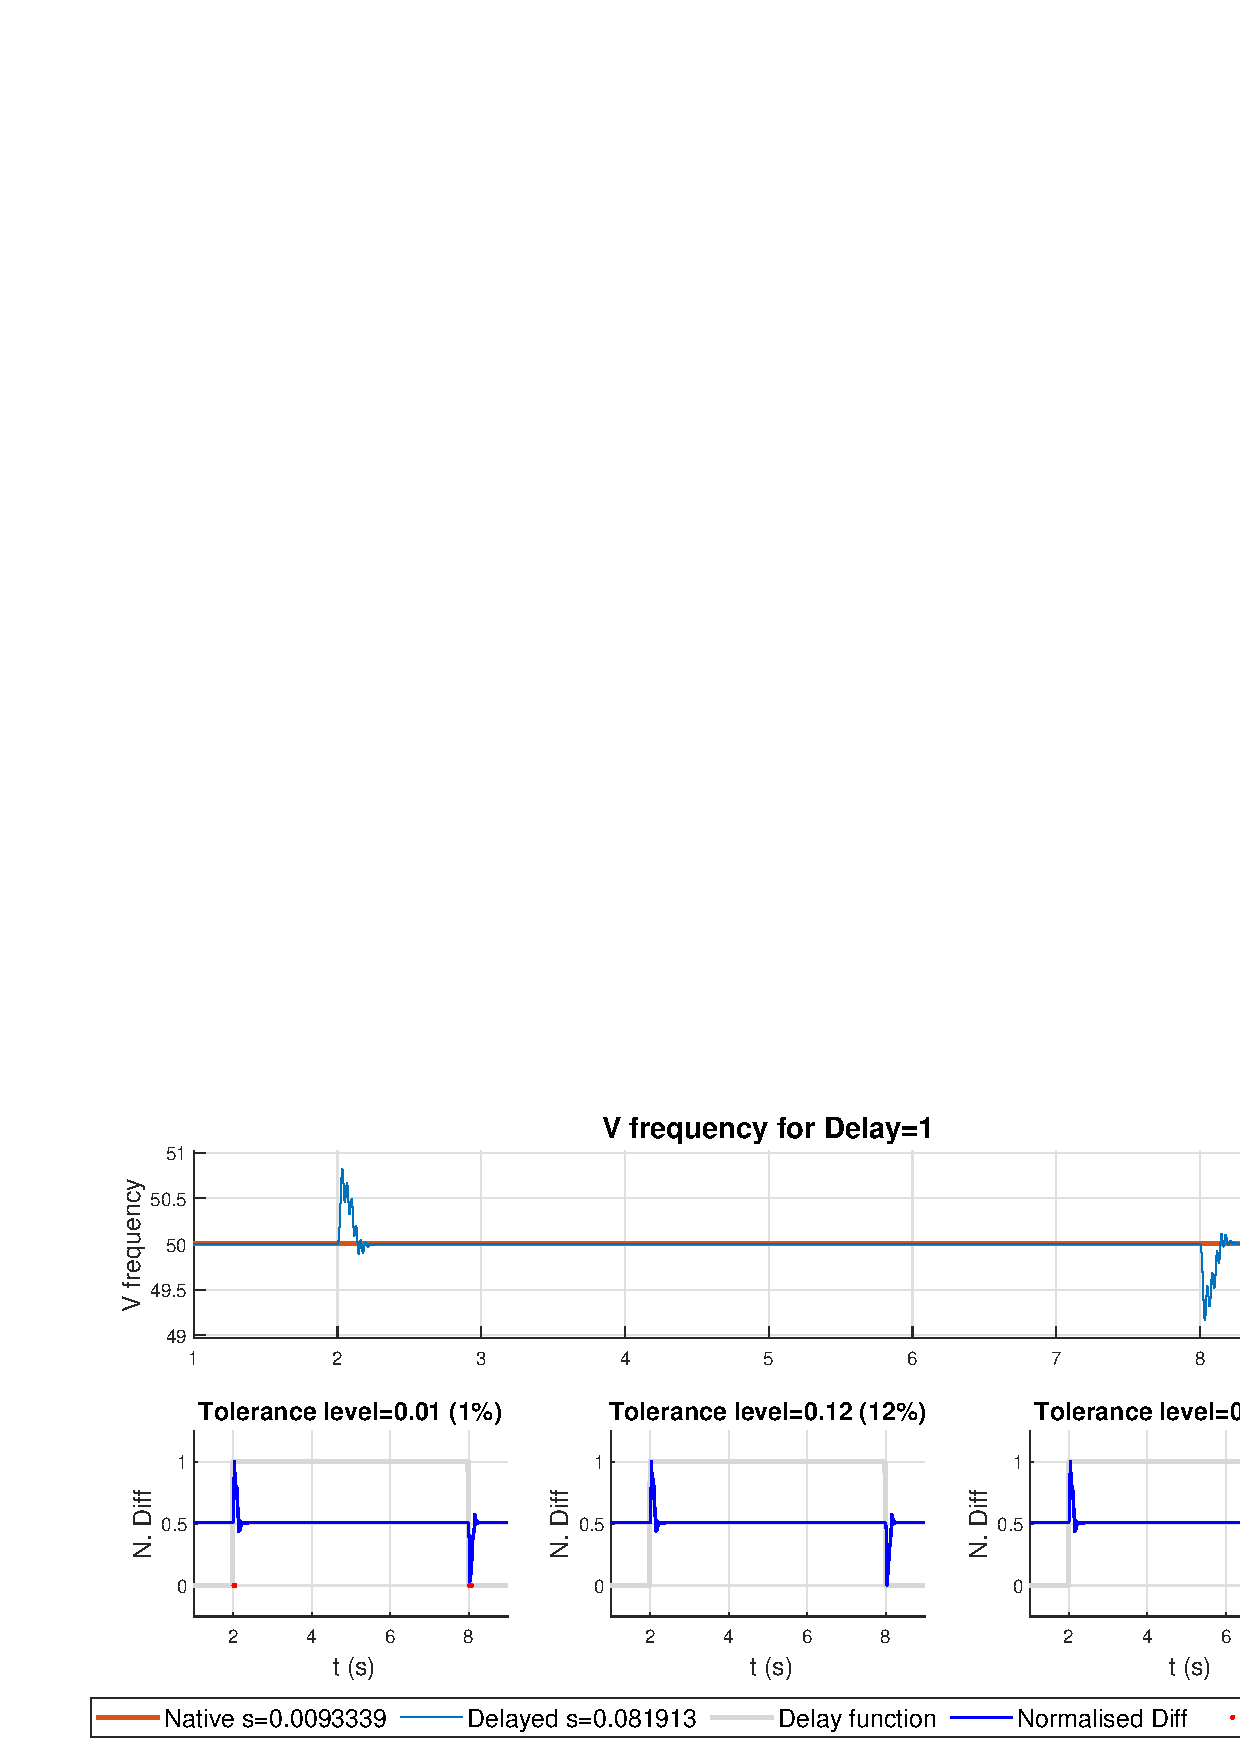
\includegraphics[width=0.95\textwidth]{PMUsim-figures/DelayOf_1/Instant_vFrequency.png}}

 
  \end{tabular}
\caption{Results for Voltage Output for Instant Delay equal to One } 
\label{fig:VoltageInstantDelayOne}
\end{figure}

\newpage
\begin{figure}[H]
\begin{tabular}{c}
  \fbox{  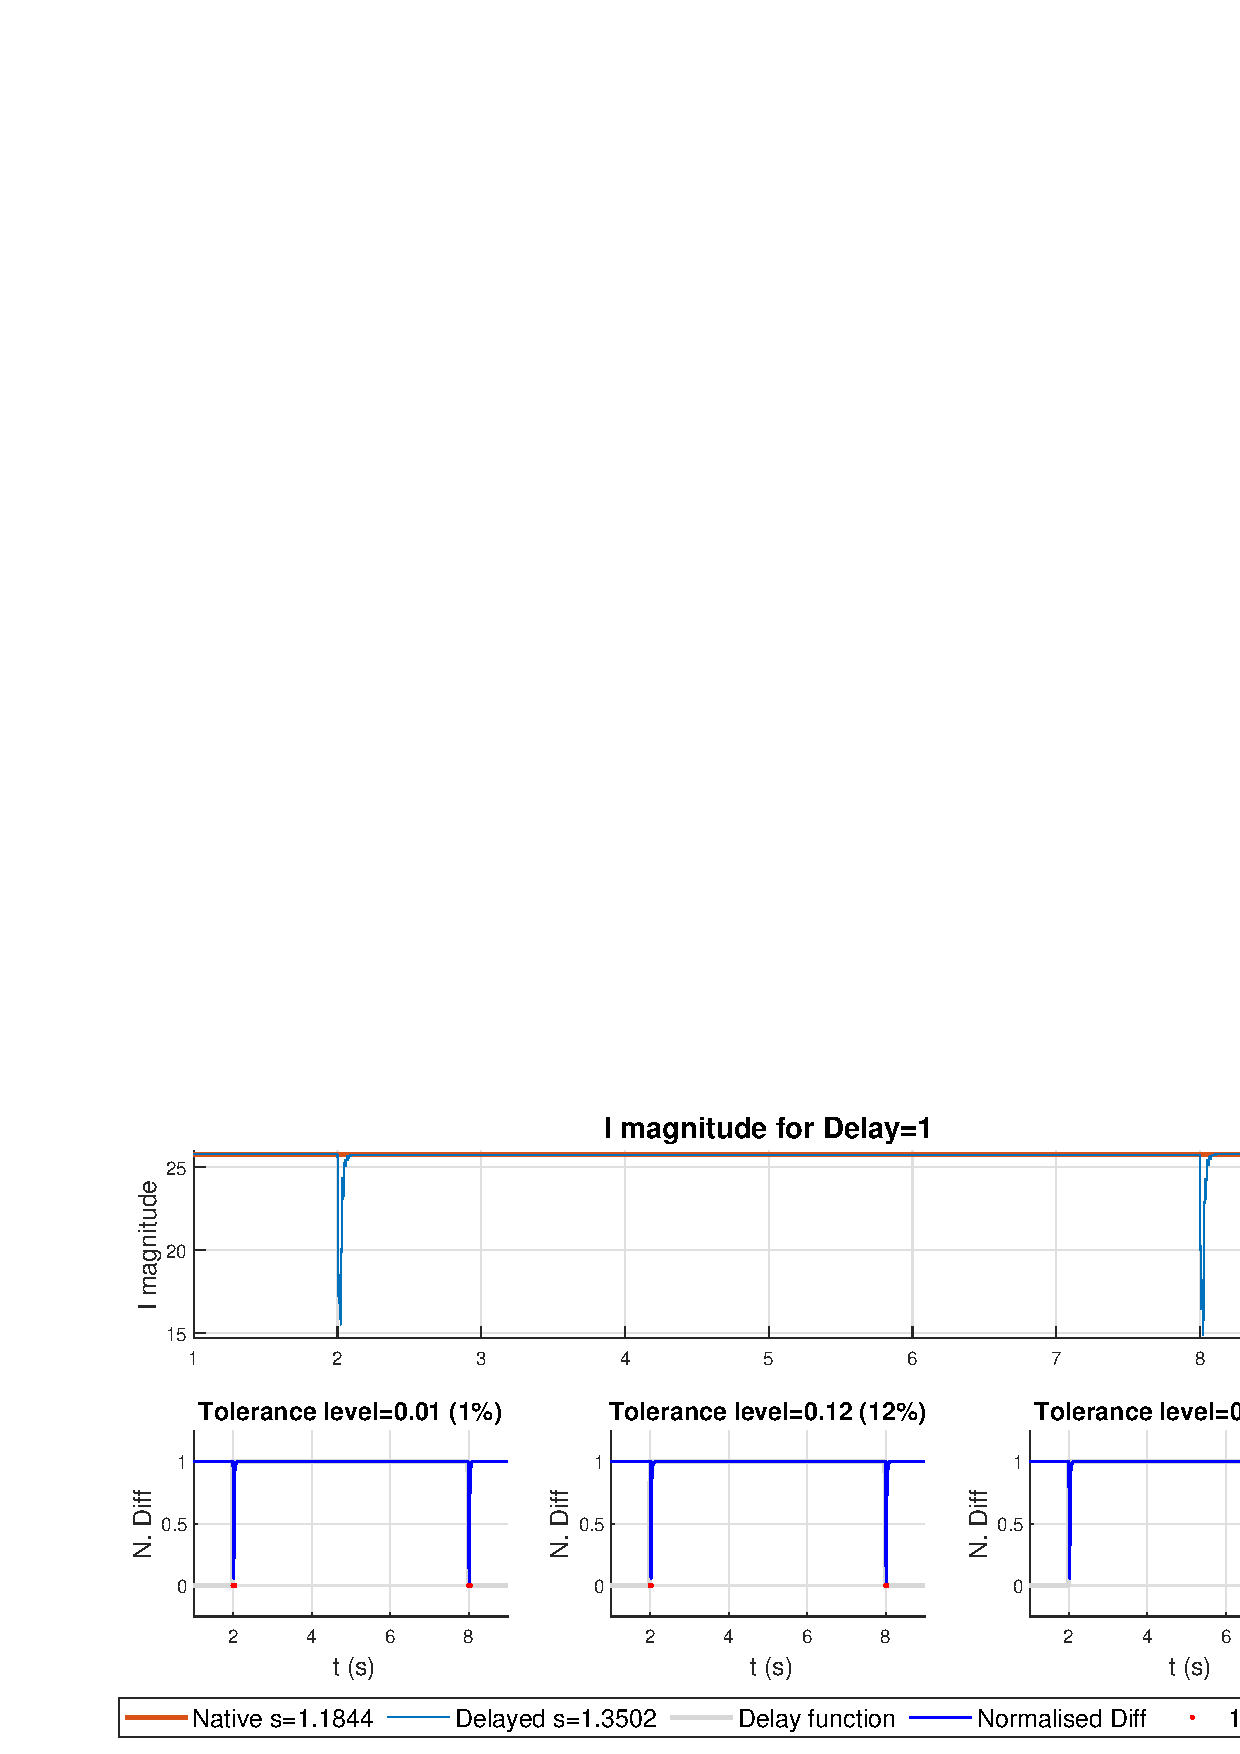
\includegraphics[width=0.95\textwidth]{PMUsim-figures/DelayOf_1/Instant_iMagnitude.png}} \\ 
    \fbox{     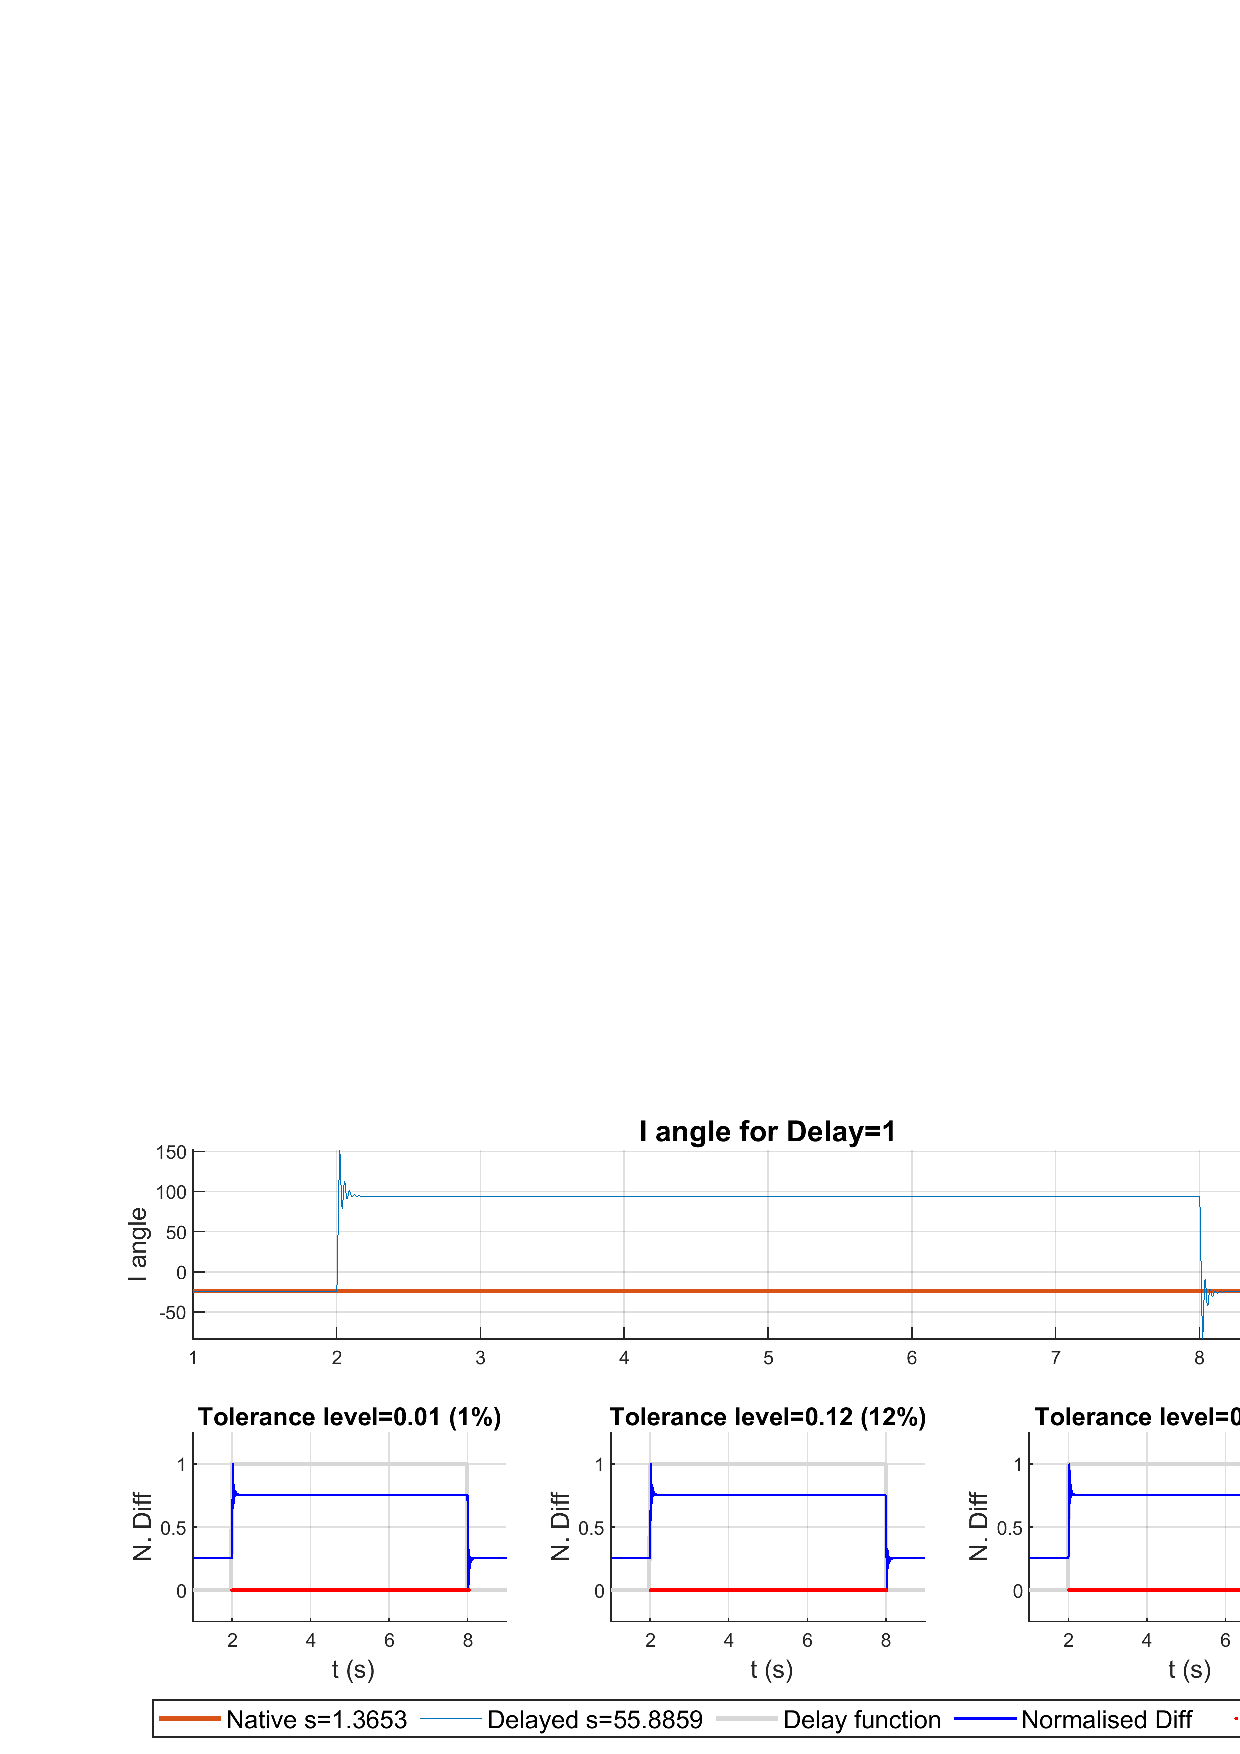
\includegraphics[width=0.95\textwidth]{PMUsim-figures/DelayOf_1/Instant_iAngle.png}} \\   
   \fbox{    \includegraphics[width=0.95\textwidth]{PMUsim-figures/DelayOf_1/Instant_iFrequency.png}}


  \end{tabular}
\label{fig:ImpedanceInstantDelayOne} 
\caption{Results for Impedance Output for Instant Delay equal to One }
\end{figure}



\newpage
\begin{figure}[H]
\begin{tabular}{c}
  \fbox{  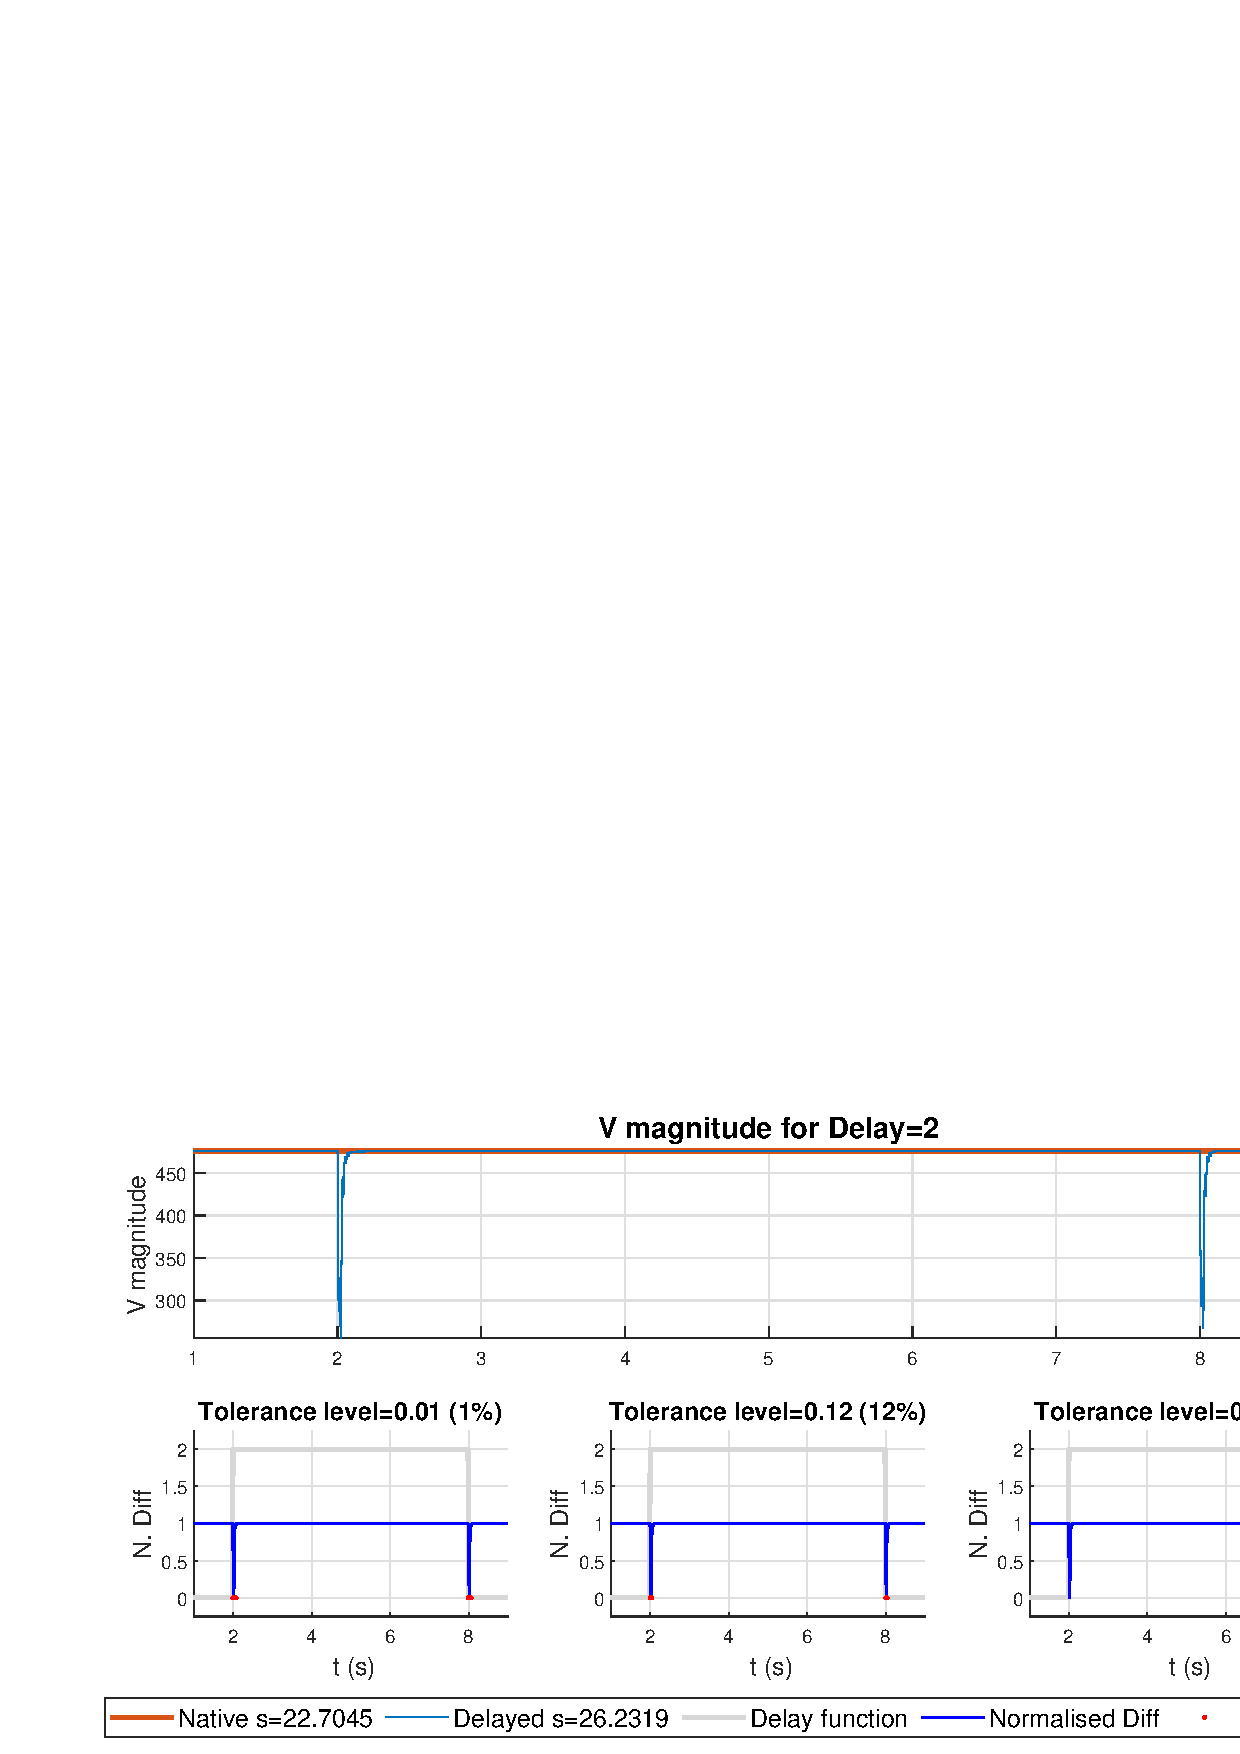
\includegraphics[width=0.95\textwidth]{PMUsim-figures/DelayOf_2/Instant_vMagnitude.png}} \\ 
    \fbox{     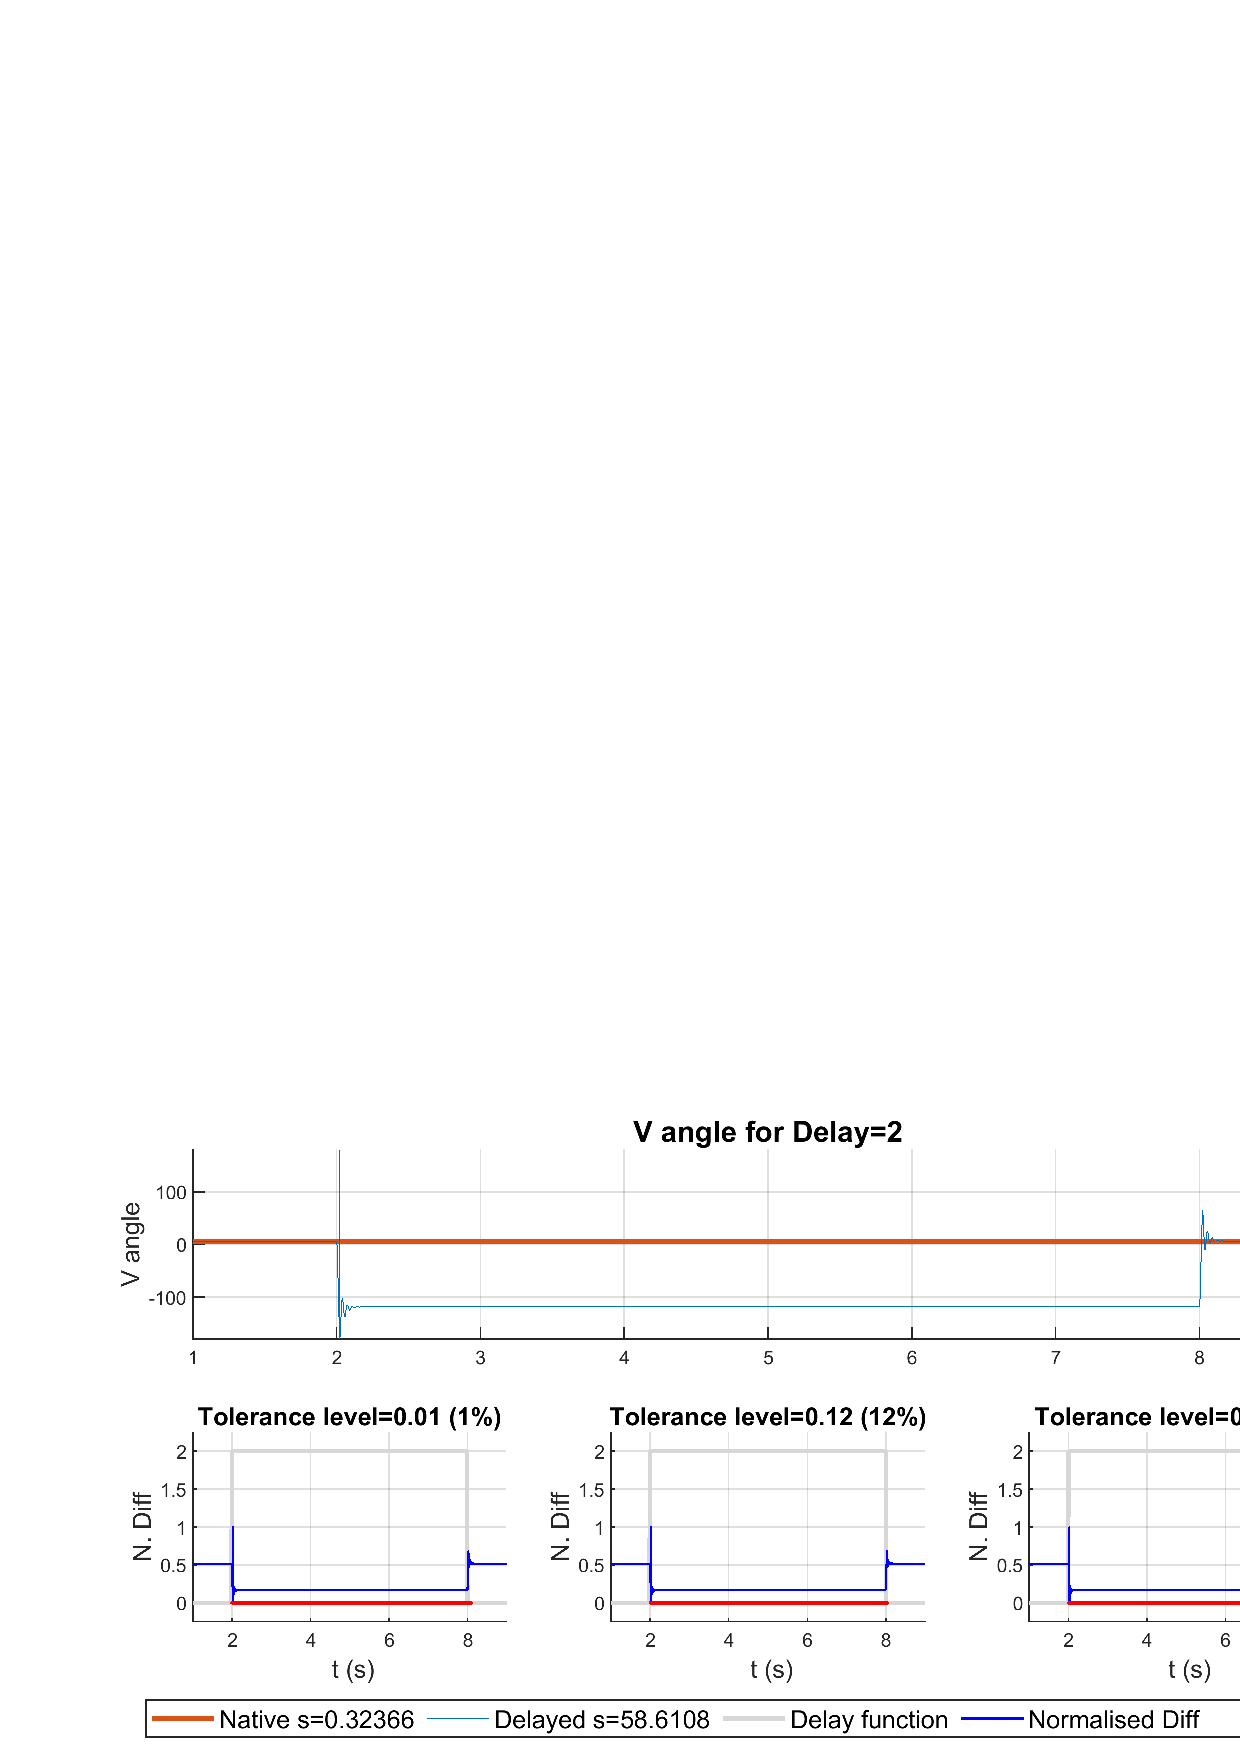
\includegraphics[width=0.95\textwidth]{PMUsim-figures/DelayOf_2/Instant_vAngle.png}} \\  
   \fbox{    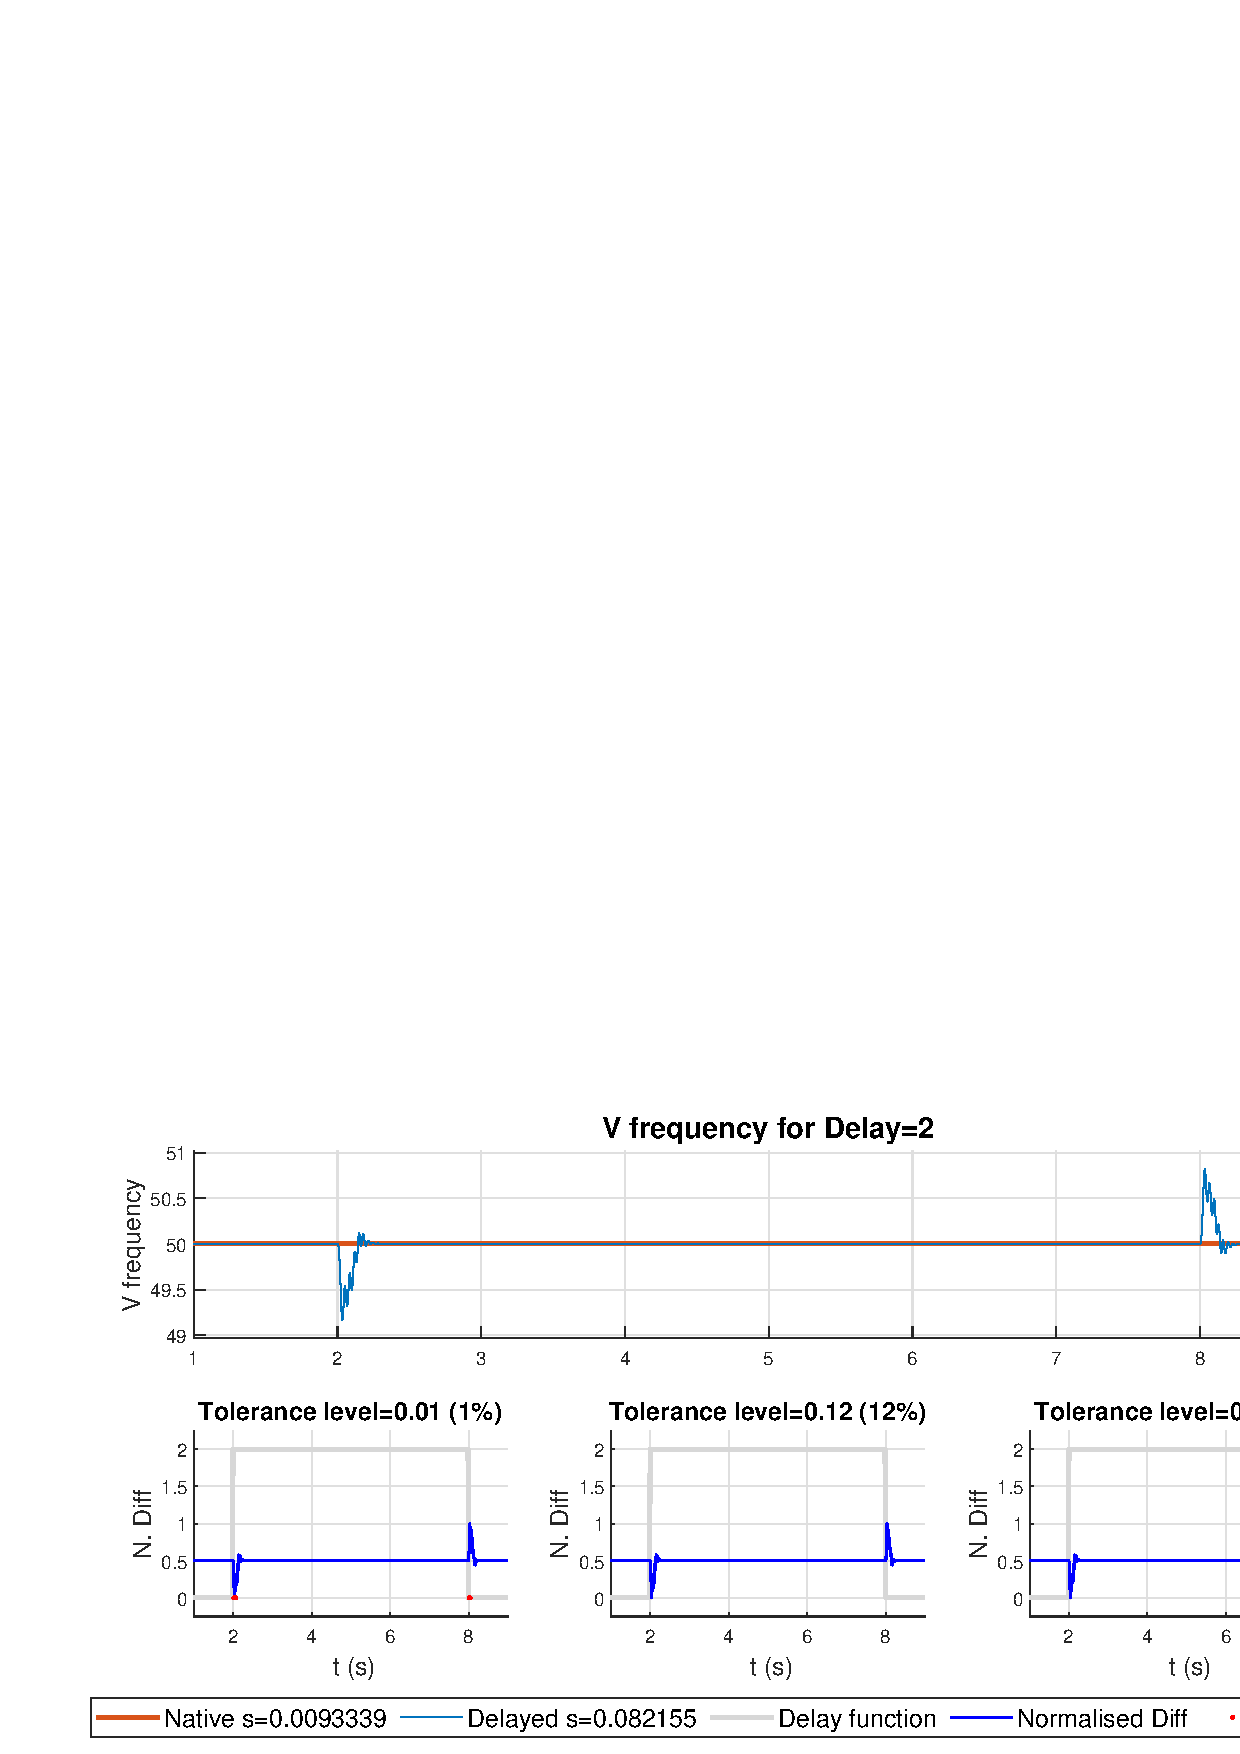
\includegraphics[width=0.95\textwidth]{PMUsim-figures/DelayOf_2/Instant_vFrequency.png}}

 
  \end{tabular}
\label{fig:VoltageInstantDelayTwo}
\caption{Results for Voltage Output for Instant Delay equal to Two }
\end{figure}

\newpage
\begin{figure}[H]
\begin{tabular}{c}
  \fbox{  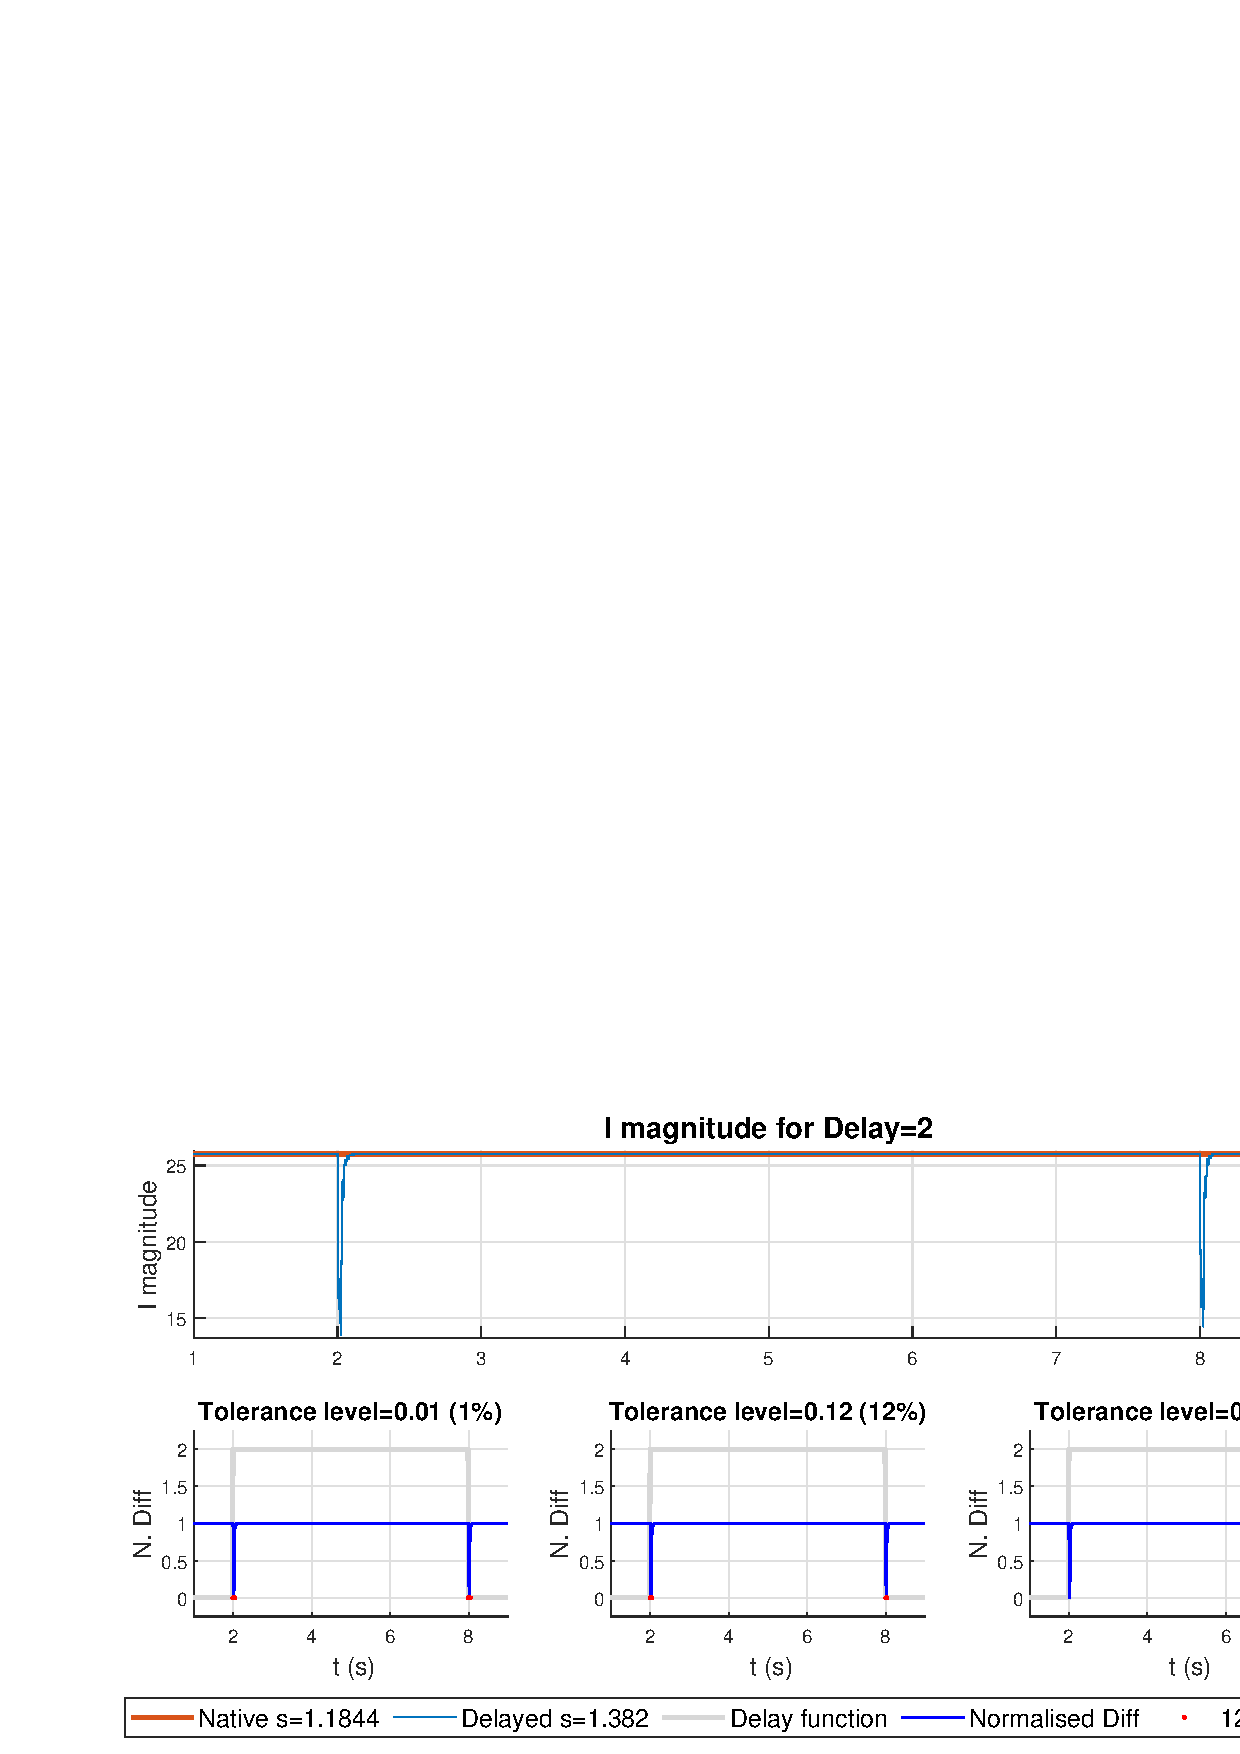
\includegraphics[width=0.95\textwidth]{PMUsim-figures/DelayOf_2/Instant_iMagnitude.png}} \\ 
    \fbox{     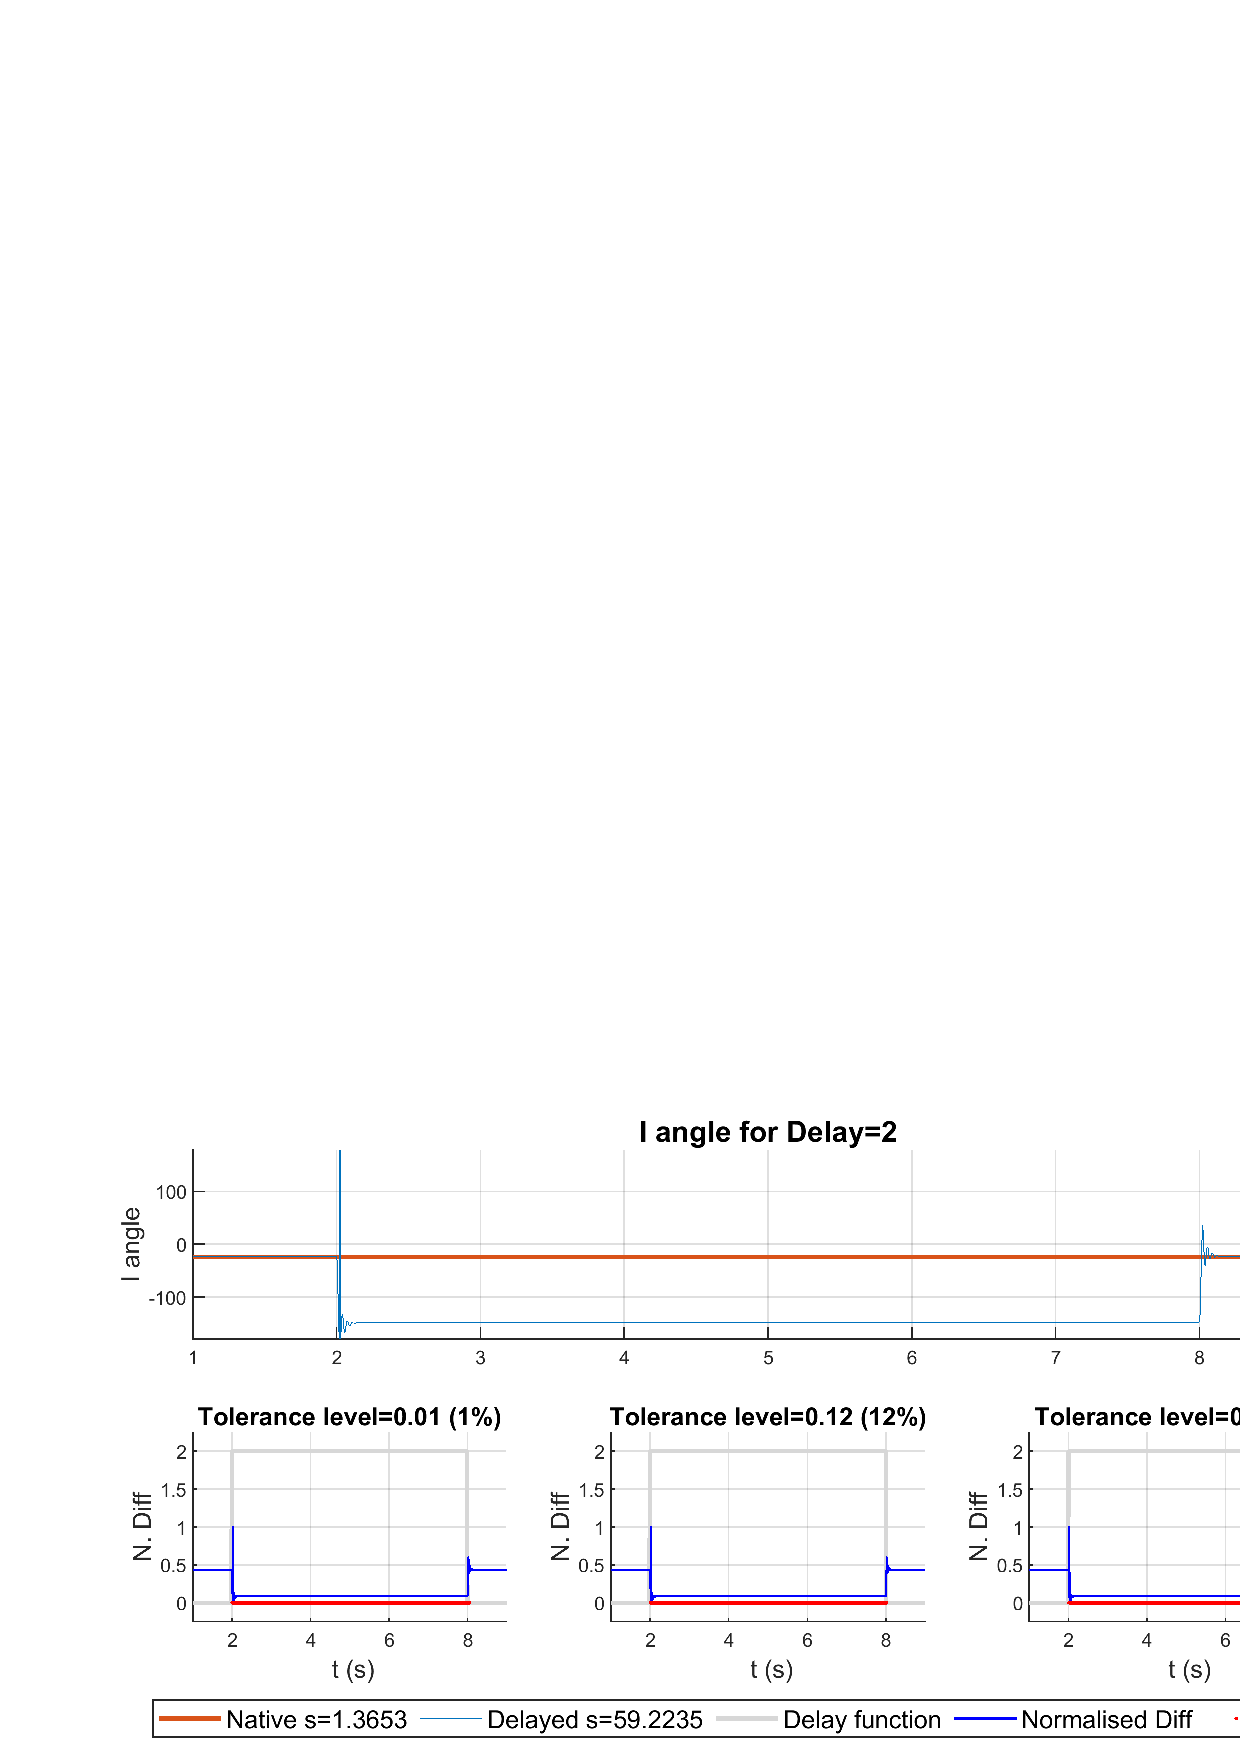
\includegraphics[width=0.95\textwidth]{PMUsim-figures/DelayOf_2/Instant_iAngle.png}} \\   
   \fbox{    \includegraphics[width=0.95\textwidth]{PMUsim-figures/DelayOf_2/Instant_iFrequency.png}}


  \end{tabular}
\label{fig:ImpedanceInstantDelayTwo}
\caption{Results for Impedance Output for Instant Delay equal to Two }
\end{figure}





\newpage
\begin{figure}[H]
\begin{tabular}{c}
  \fbox{  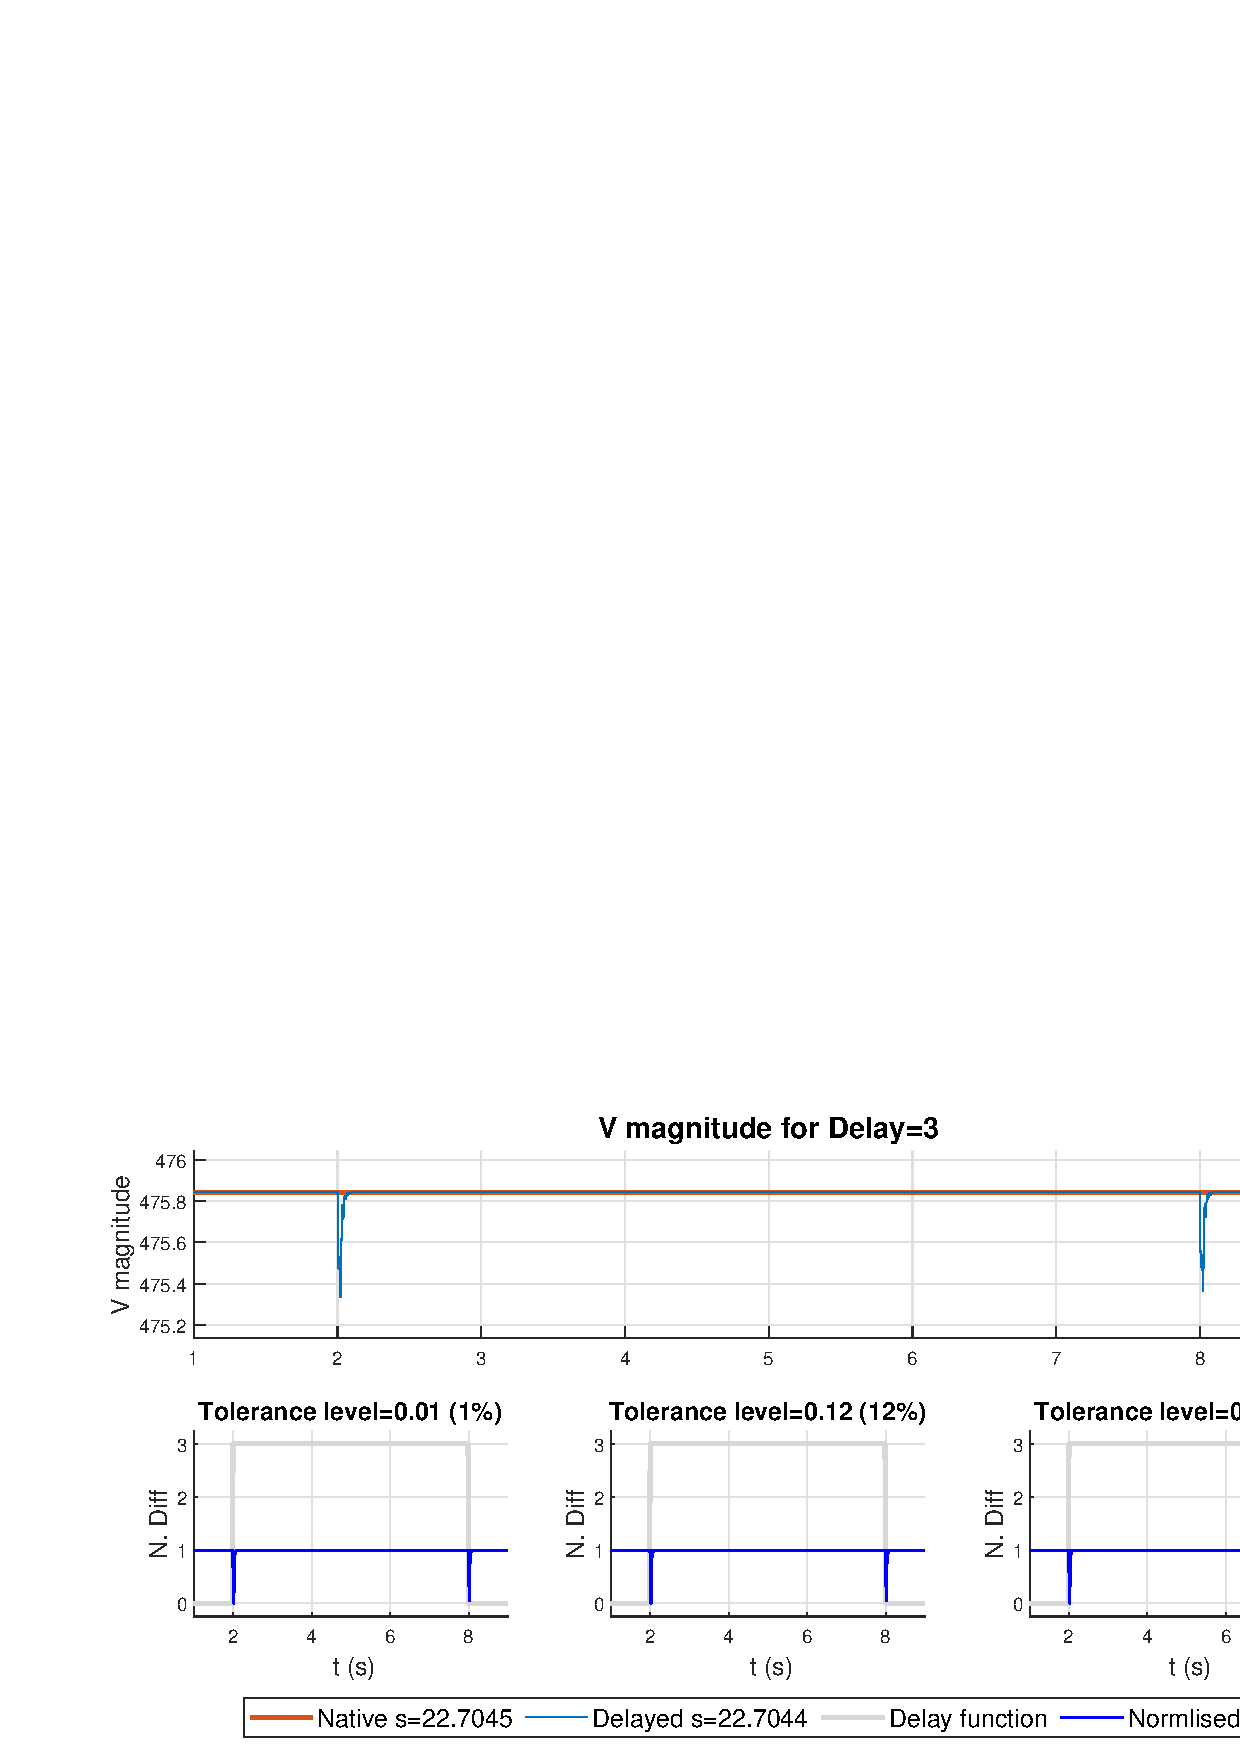
\includegraphics[width=0.95\textwidth]{PMUsim-figures/DelayOf_3/Instant_vMagnitude.png}} \\ 
   \fbox{     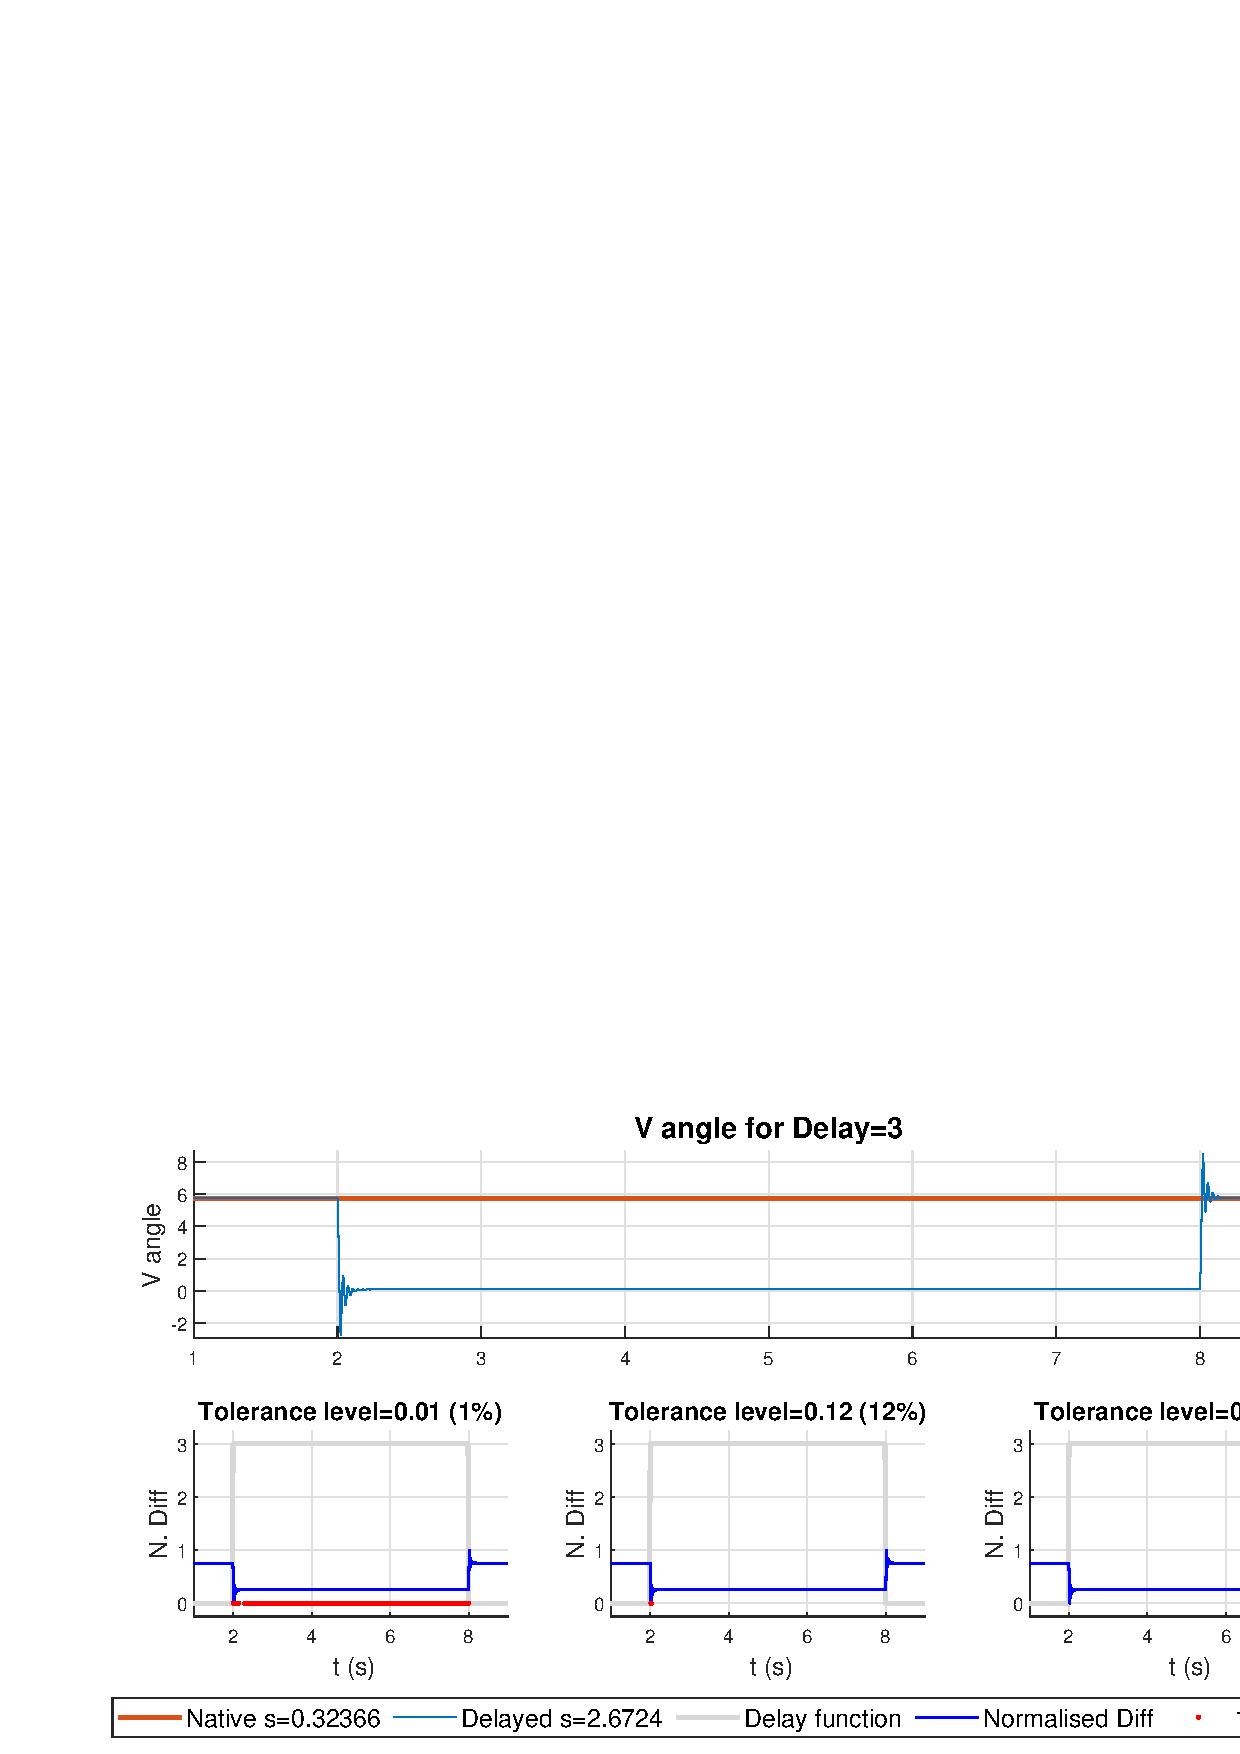
\includegraphics[width=0.95\textwidth]{PMUsim-figures/DelayOf_3/Instant_vAngle.png}} \\    
   \fbox{    \includegraphics[width=0.95\textwidth]{PMUsim-figures/DelayOf_3/Instant_vFrequency.png}}


  \end{tabular}
\label{fig:VoltageInstantDelayThree}
\caption{Results for Voltage Output for Instant Delay equal to Three }
\end{figure}

\newpage
\begin{figure}[H]
\begin{tabular}{c}
  \fbox{  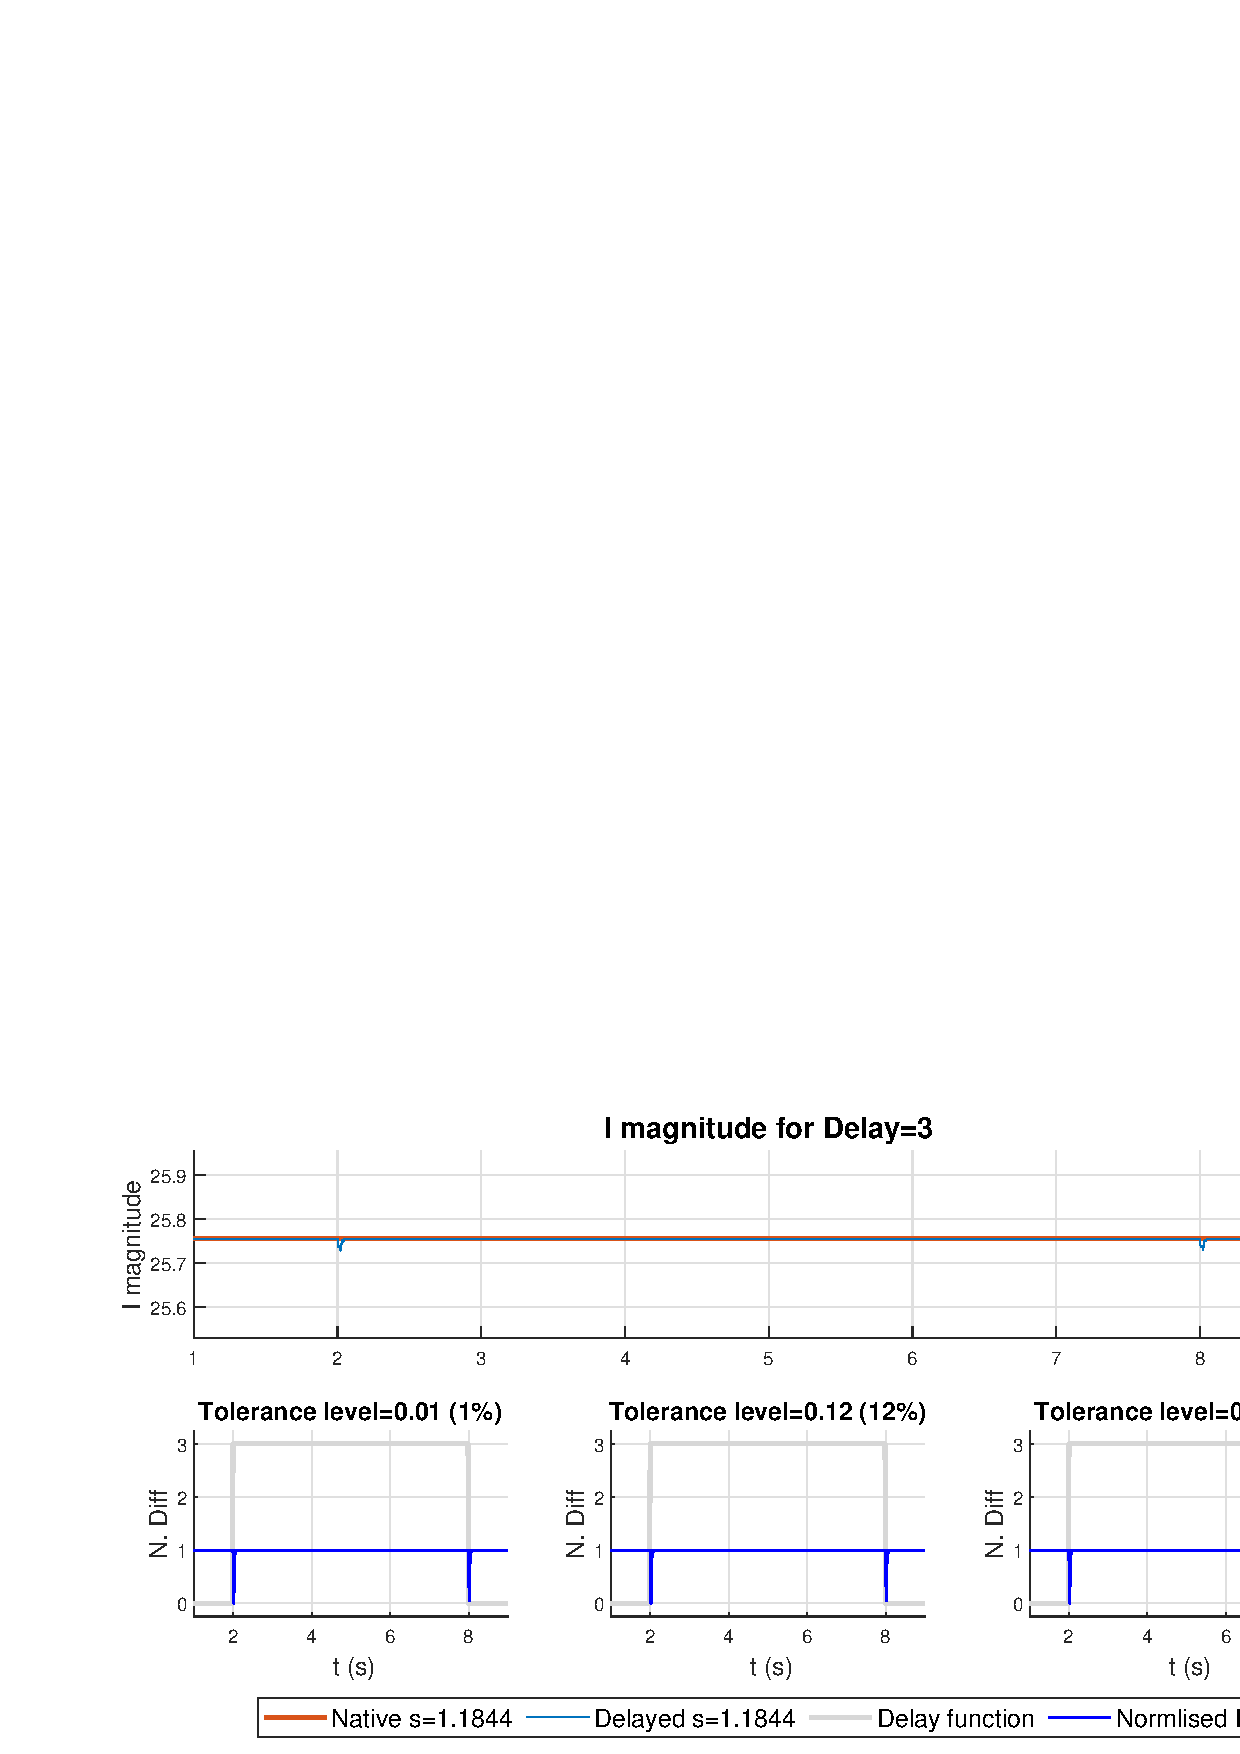
\includegraphics[width=0.95\textwidth]{PMUsim-figures/DelayOf_3/Instant_iMagnitude.png}} \\ 
   \fbox{     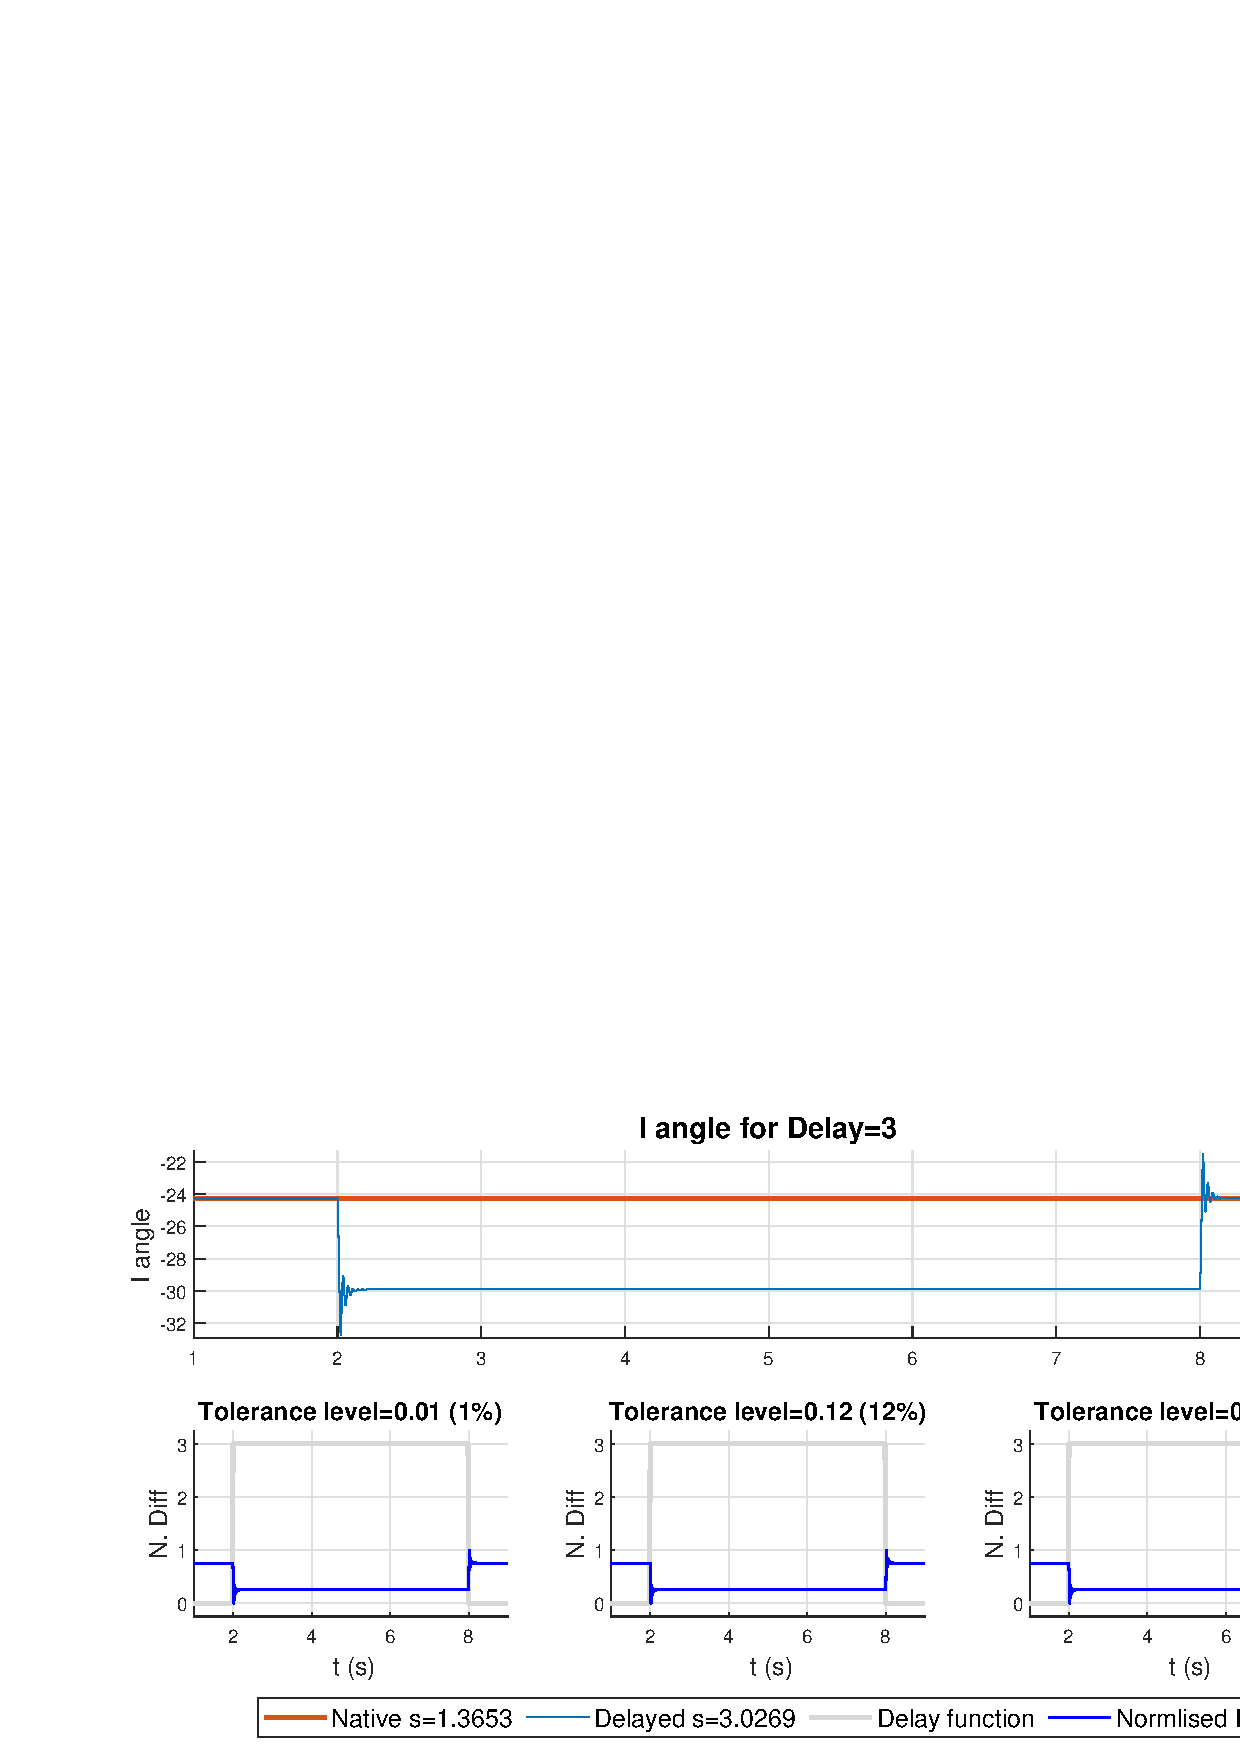
\includegraphics[width=0.95\textwidth]{PMUsim-figures/DelayOf_3/Instant_iAngle.png}} \\    
   \fbox{    \includegraphics[width=0.95\textwidth]{PMUsim-figures/DelayOf_3/Instant_iFrequency.png}}


  \end{tabular}
\label{fig:ImpedanceInstantDelayThree}
\caption{Results for Impedance Output for Instant Delay equal to Three }
\end{figure}






\newpage
\begin{figure}[H]
\begin{tabular}{c}
  \fbox{  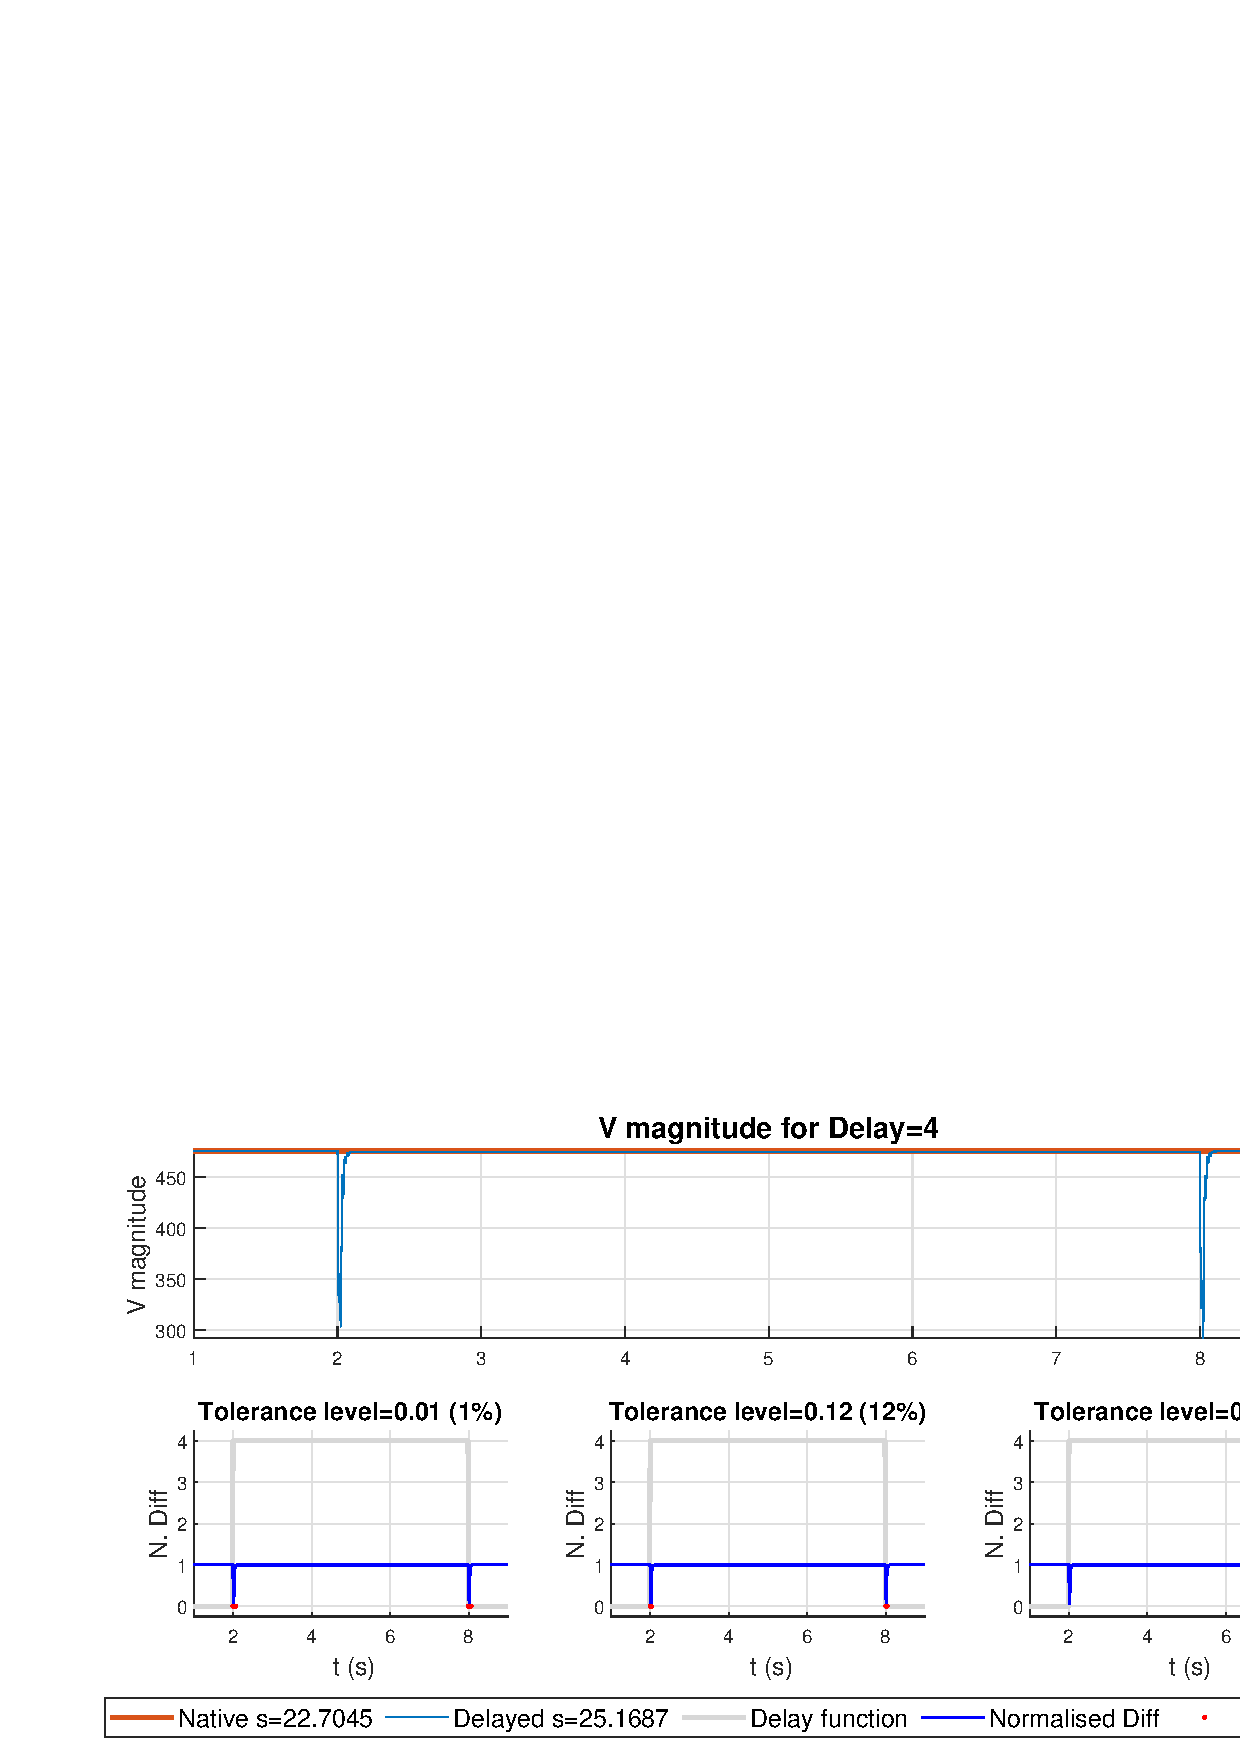
\includegraphics[width=0.95\textwidth]{PMUsim-figures/DelayOf_4/Instant_vMagnitude.png}} \\ 
  \fbox{     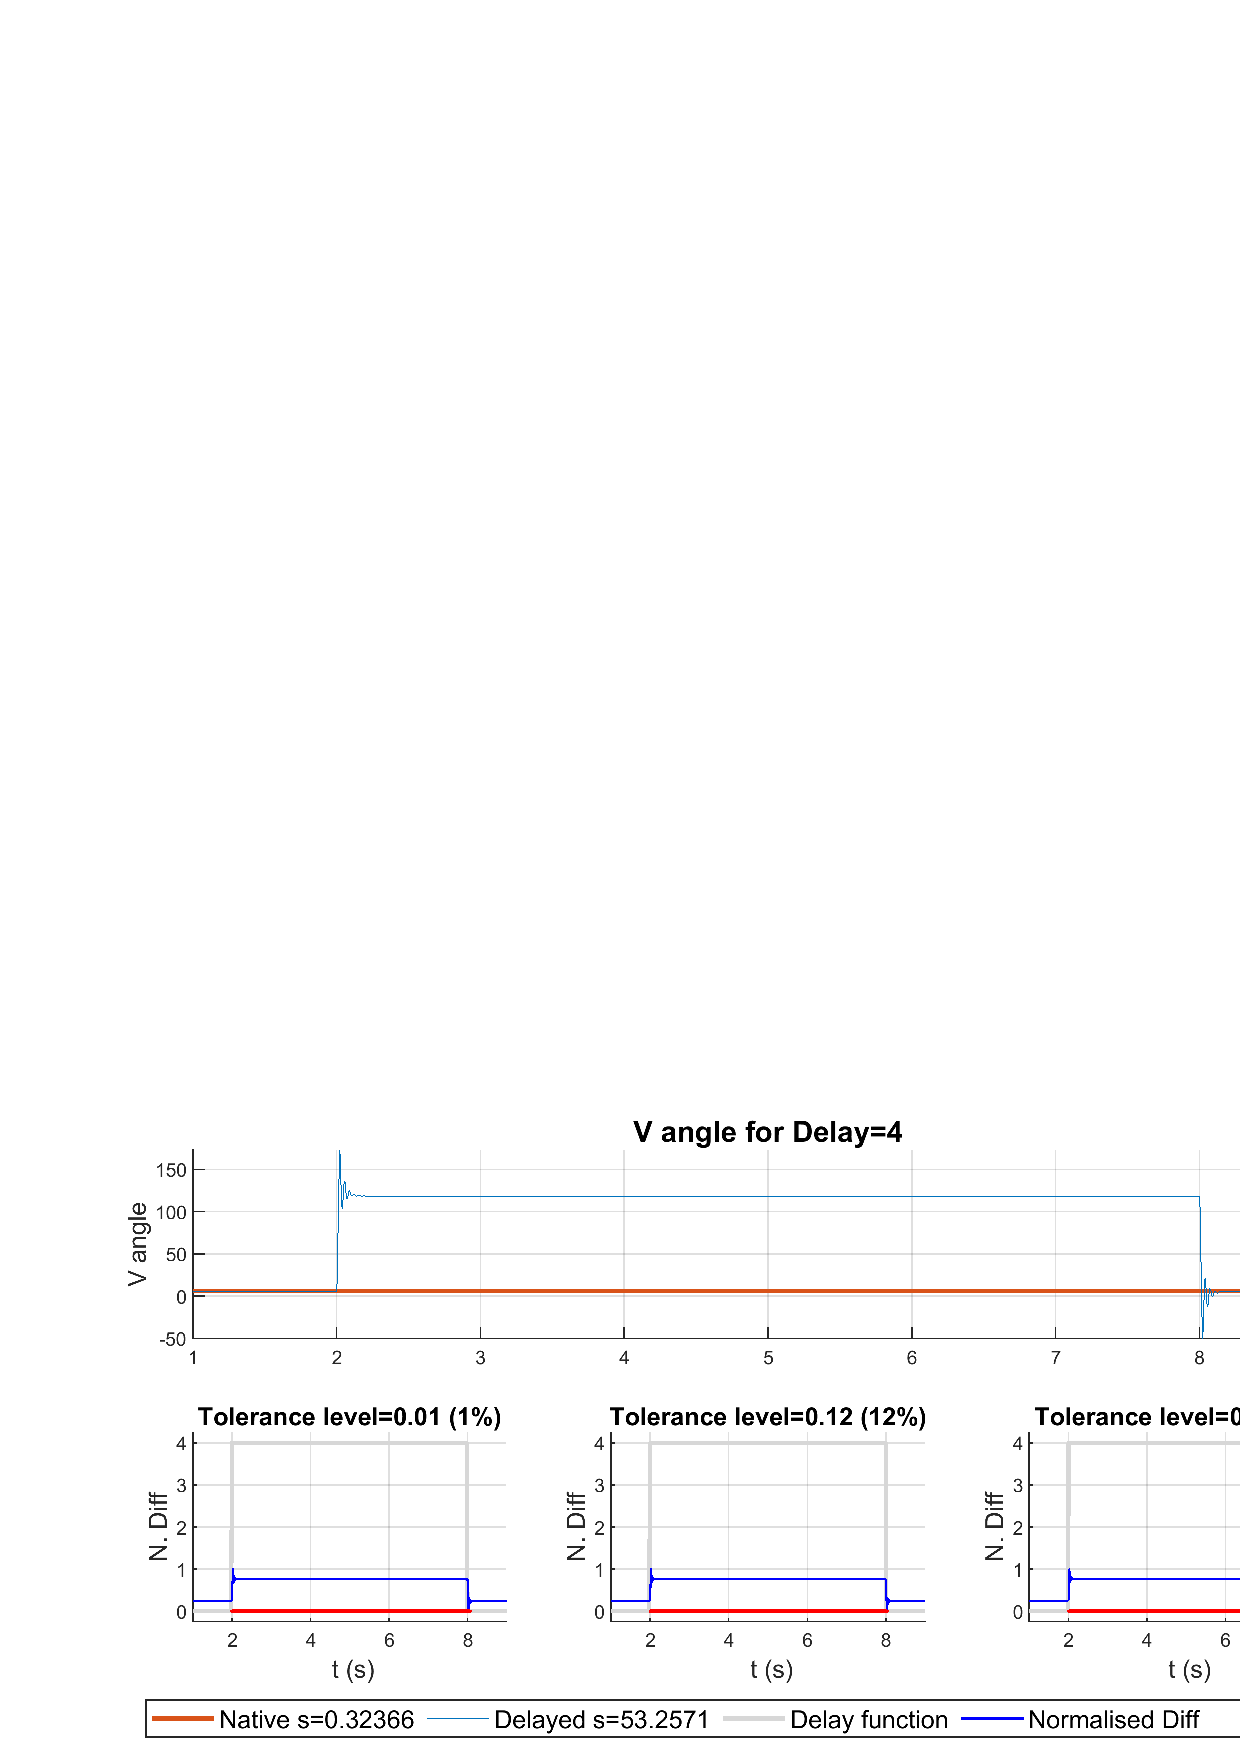
\includegraphics[width=0.95\textwidth]{PMUsim-figures/DelayOf_4/Instant_vAngle.png}} \\   
   \fbox{    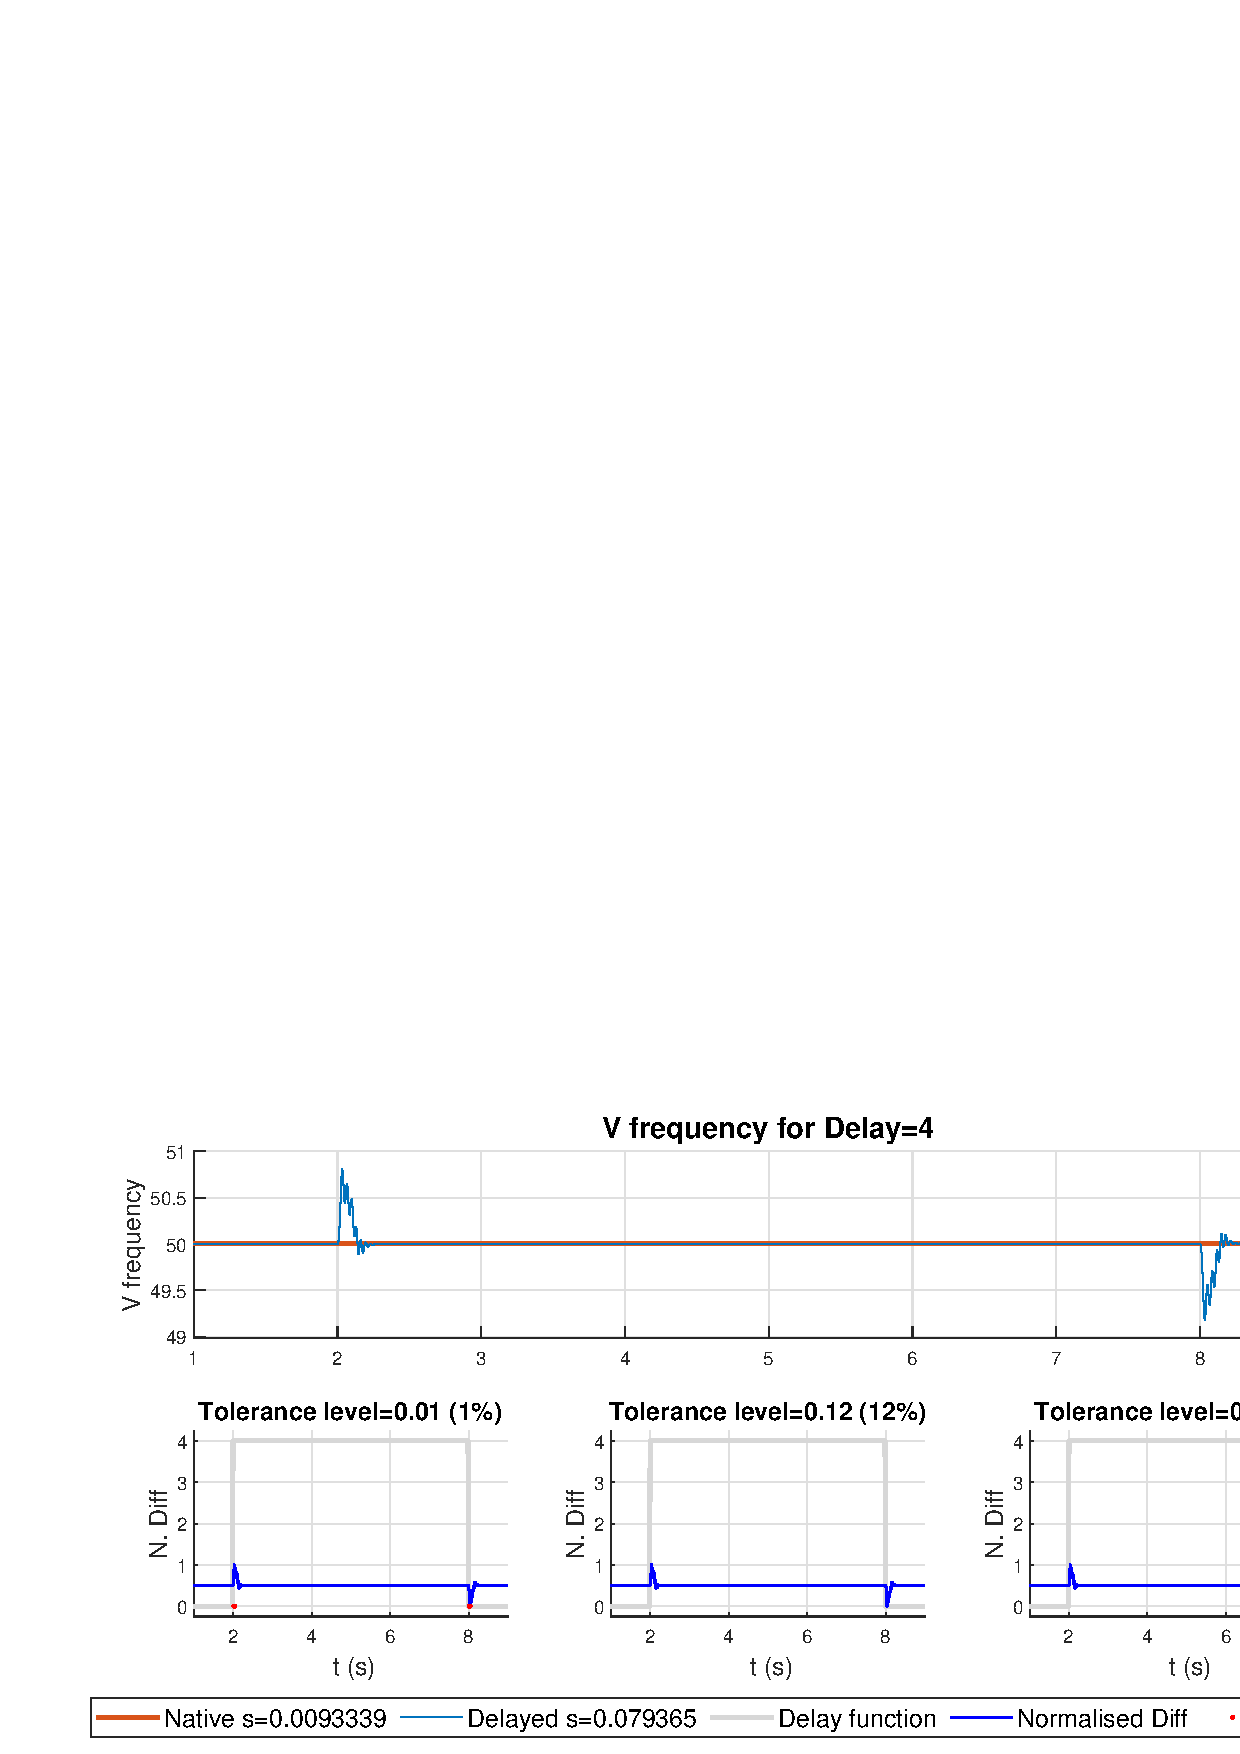
\includegraphics[width=0.95\textwidth]{PMUsim-figures/DelayOf_4/Instant_vFrequency.png}} 
 
  \end{tabular}
\label{fig:VoltageInstantDelayFour}
\caption{Results for Voltage Output for Instant Delay equal to Four }
\end{figure}

\newpage
\begin{figure}[H]
\begin{tabular}{c}
  \fbox{  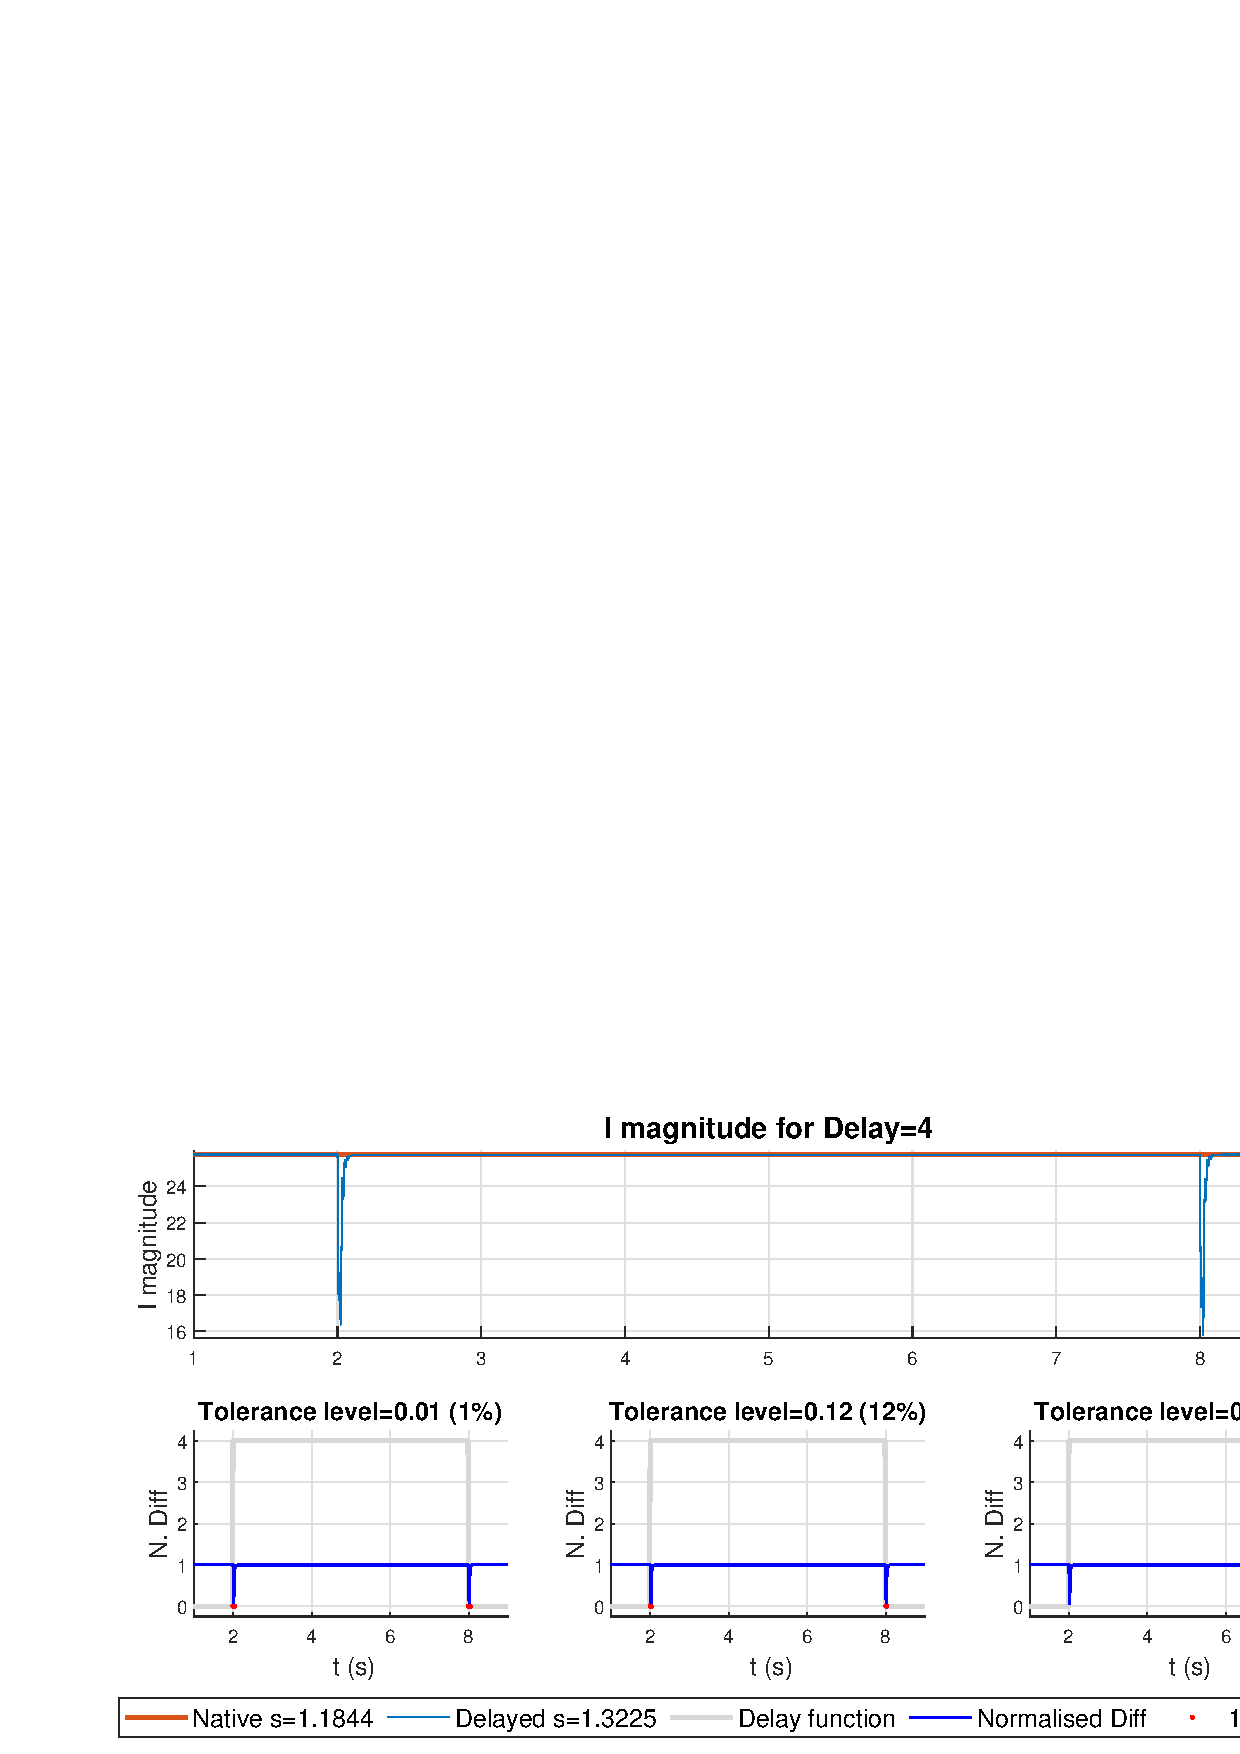
\includegraphics[width=0.95\textwidth]{PMUsim-figures/DelayOf_4/Instant_iMagnitude.png}} \\ 
   \fbox{     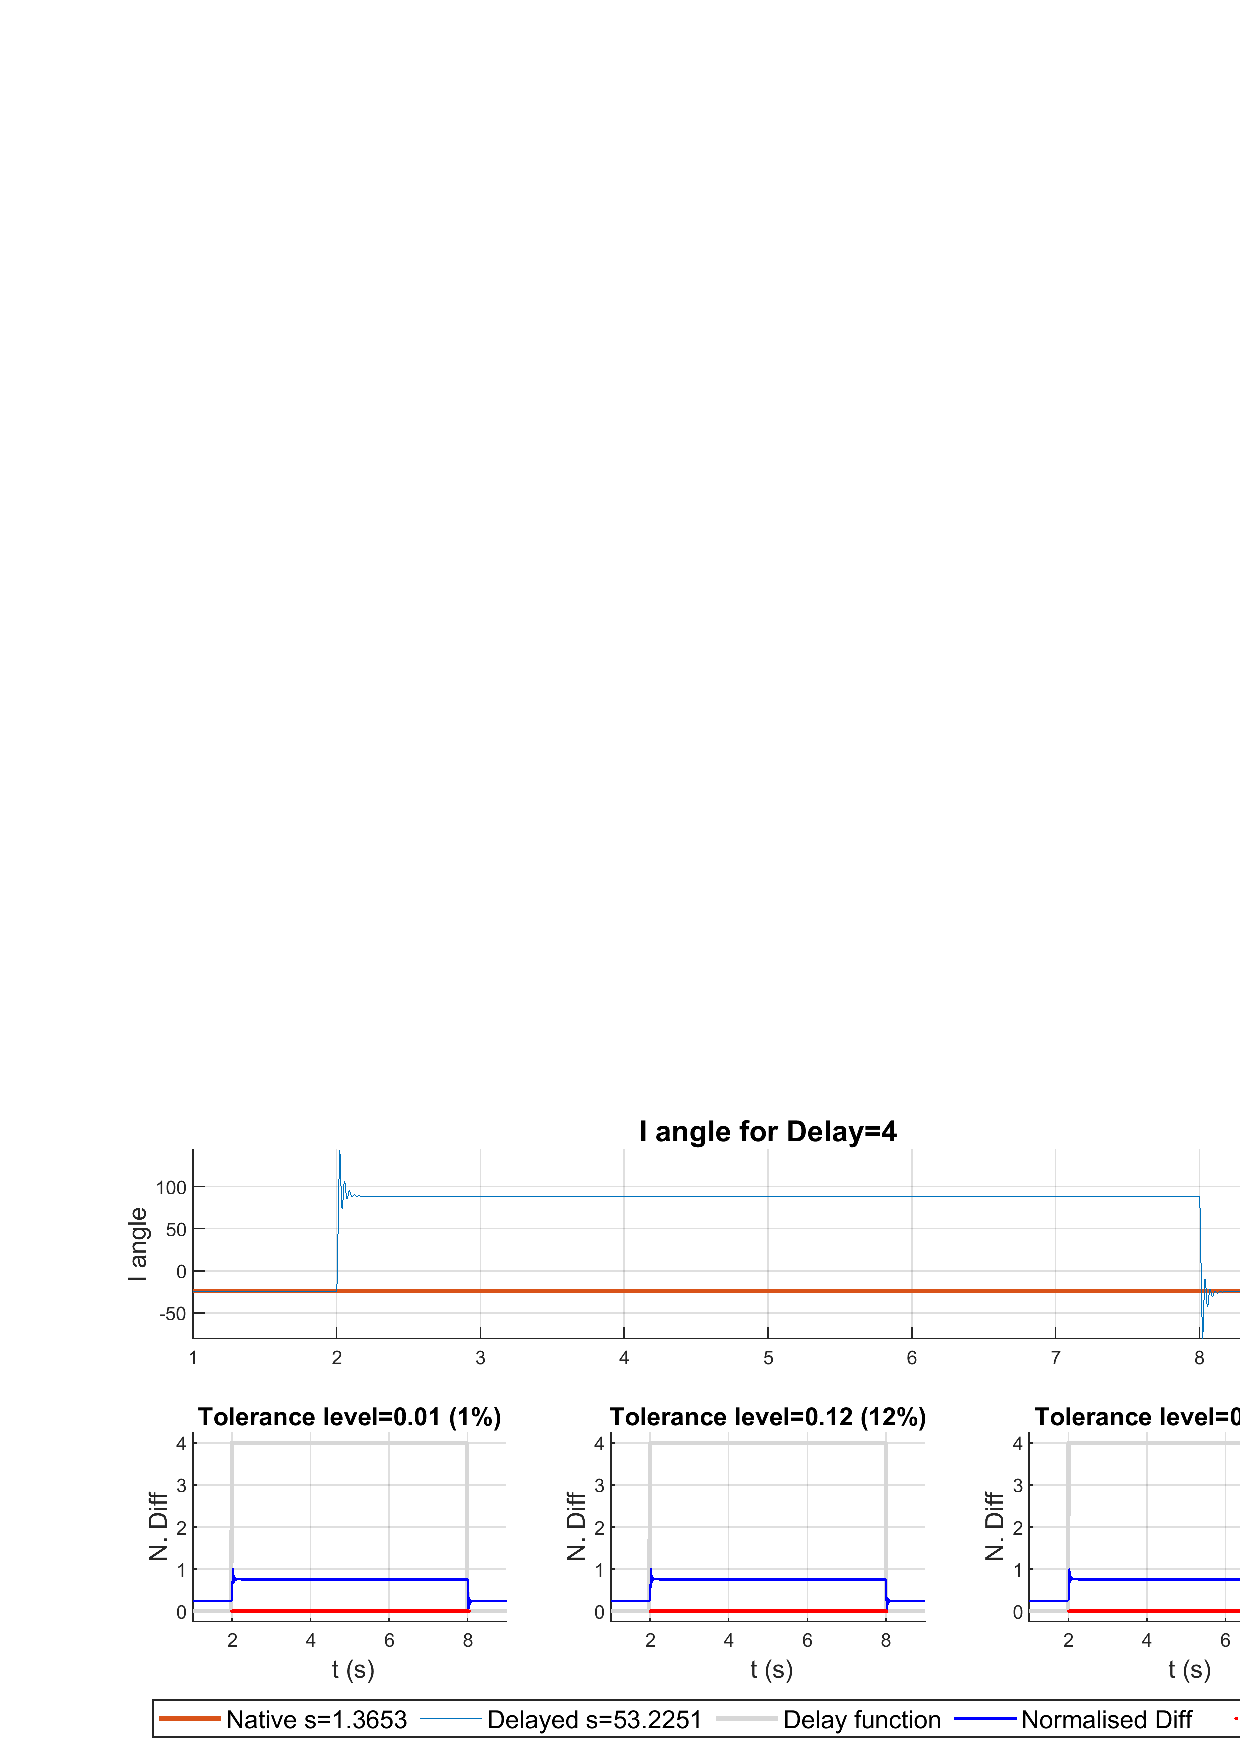
\includegraphics[width=0.95\textwidth]{PMUsim-figures/DelayOf_4/Instant_iAngle.png}} \\    
   \fbox{    \includegraphics[width=0.95\textwidth]{PMUsim-figures/DelayOf_4/Instant_iFrequency.png}}


  \end{tabular}
\label{fig:ImpedanceInstantDelayFour}
\caption{Results for Impedance Output for Instant Delay equal to Four }
\end{figure}




\newpage
\begin{figure}[H]
\begin{tabular}{c}
  \fbox{  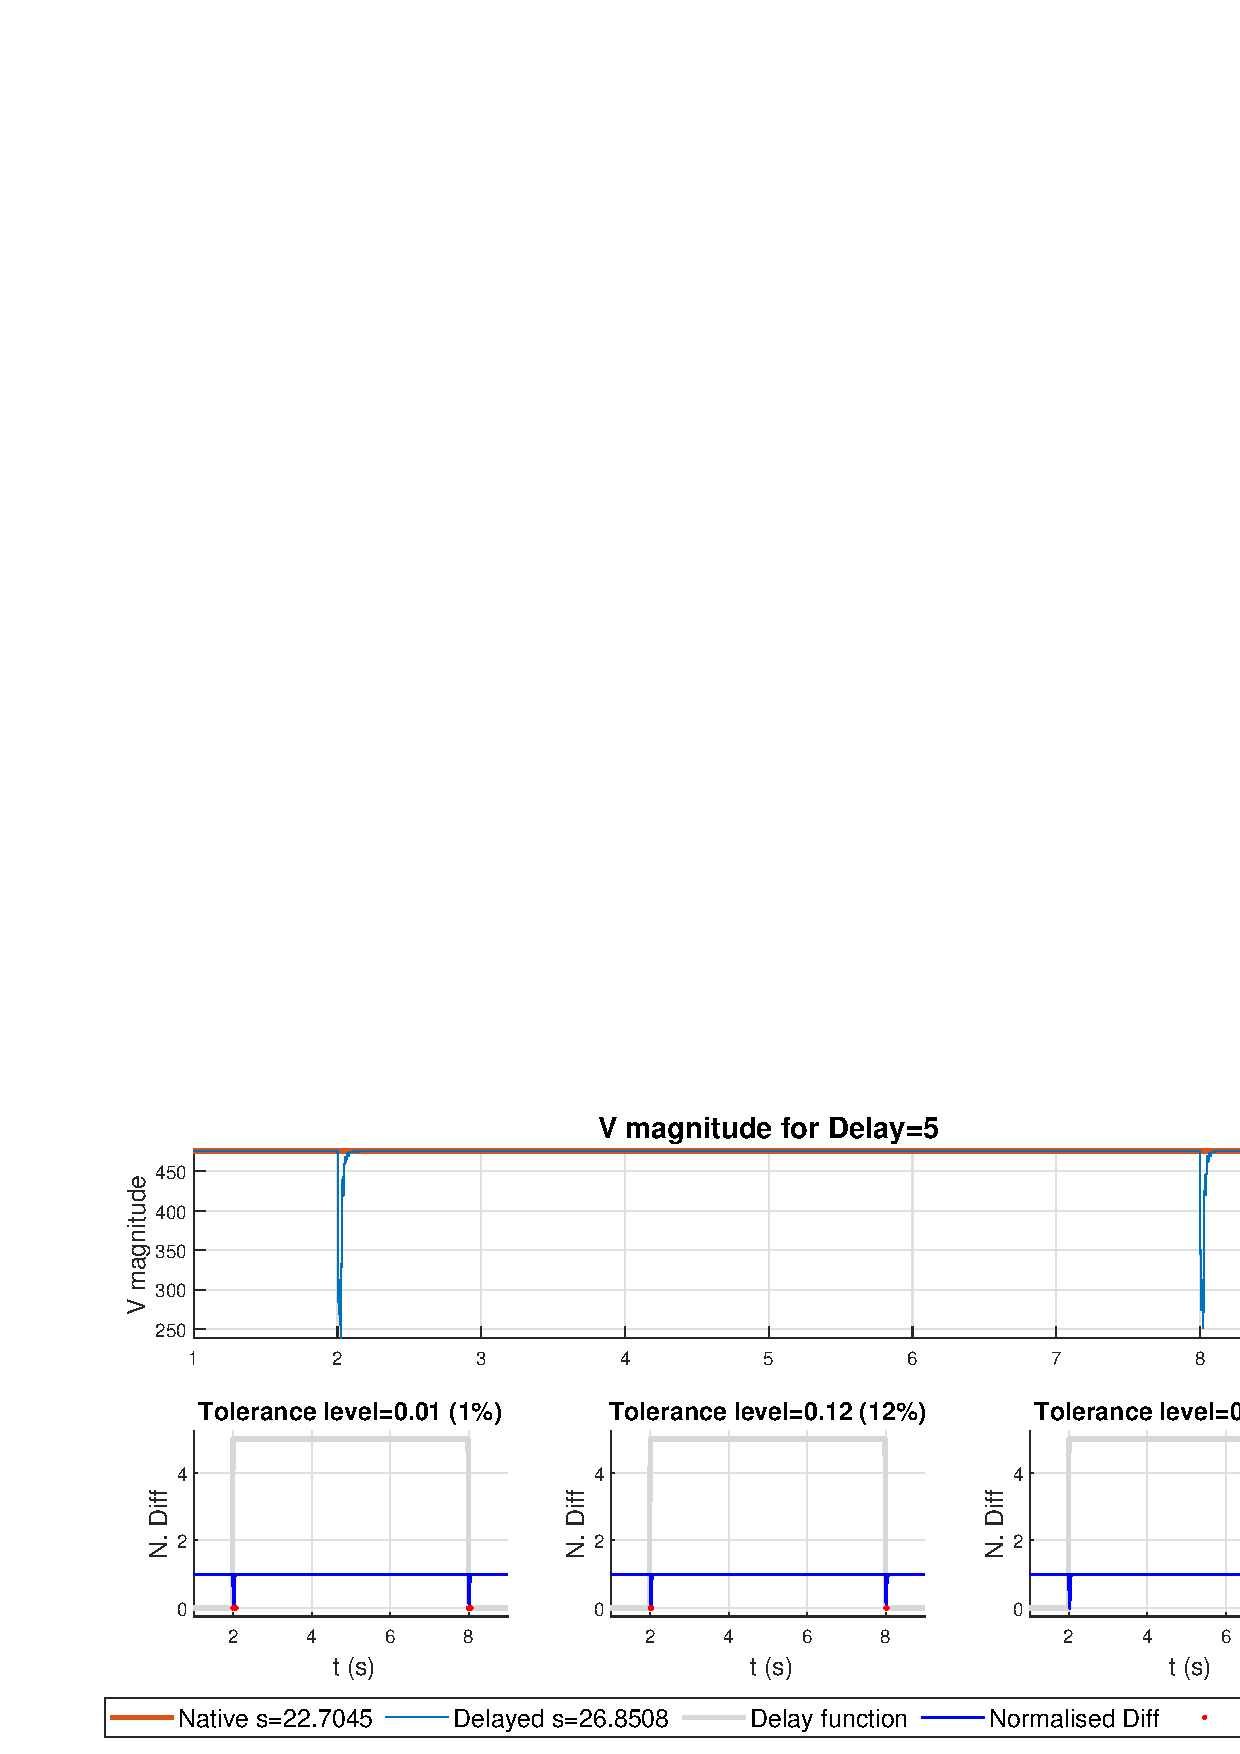
\includegraphics[width=0.95\textwidth]{PMUsim-figures/DelayOf_5/Instant_vMagnitude.png}} \\ 
    \fbox{     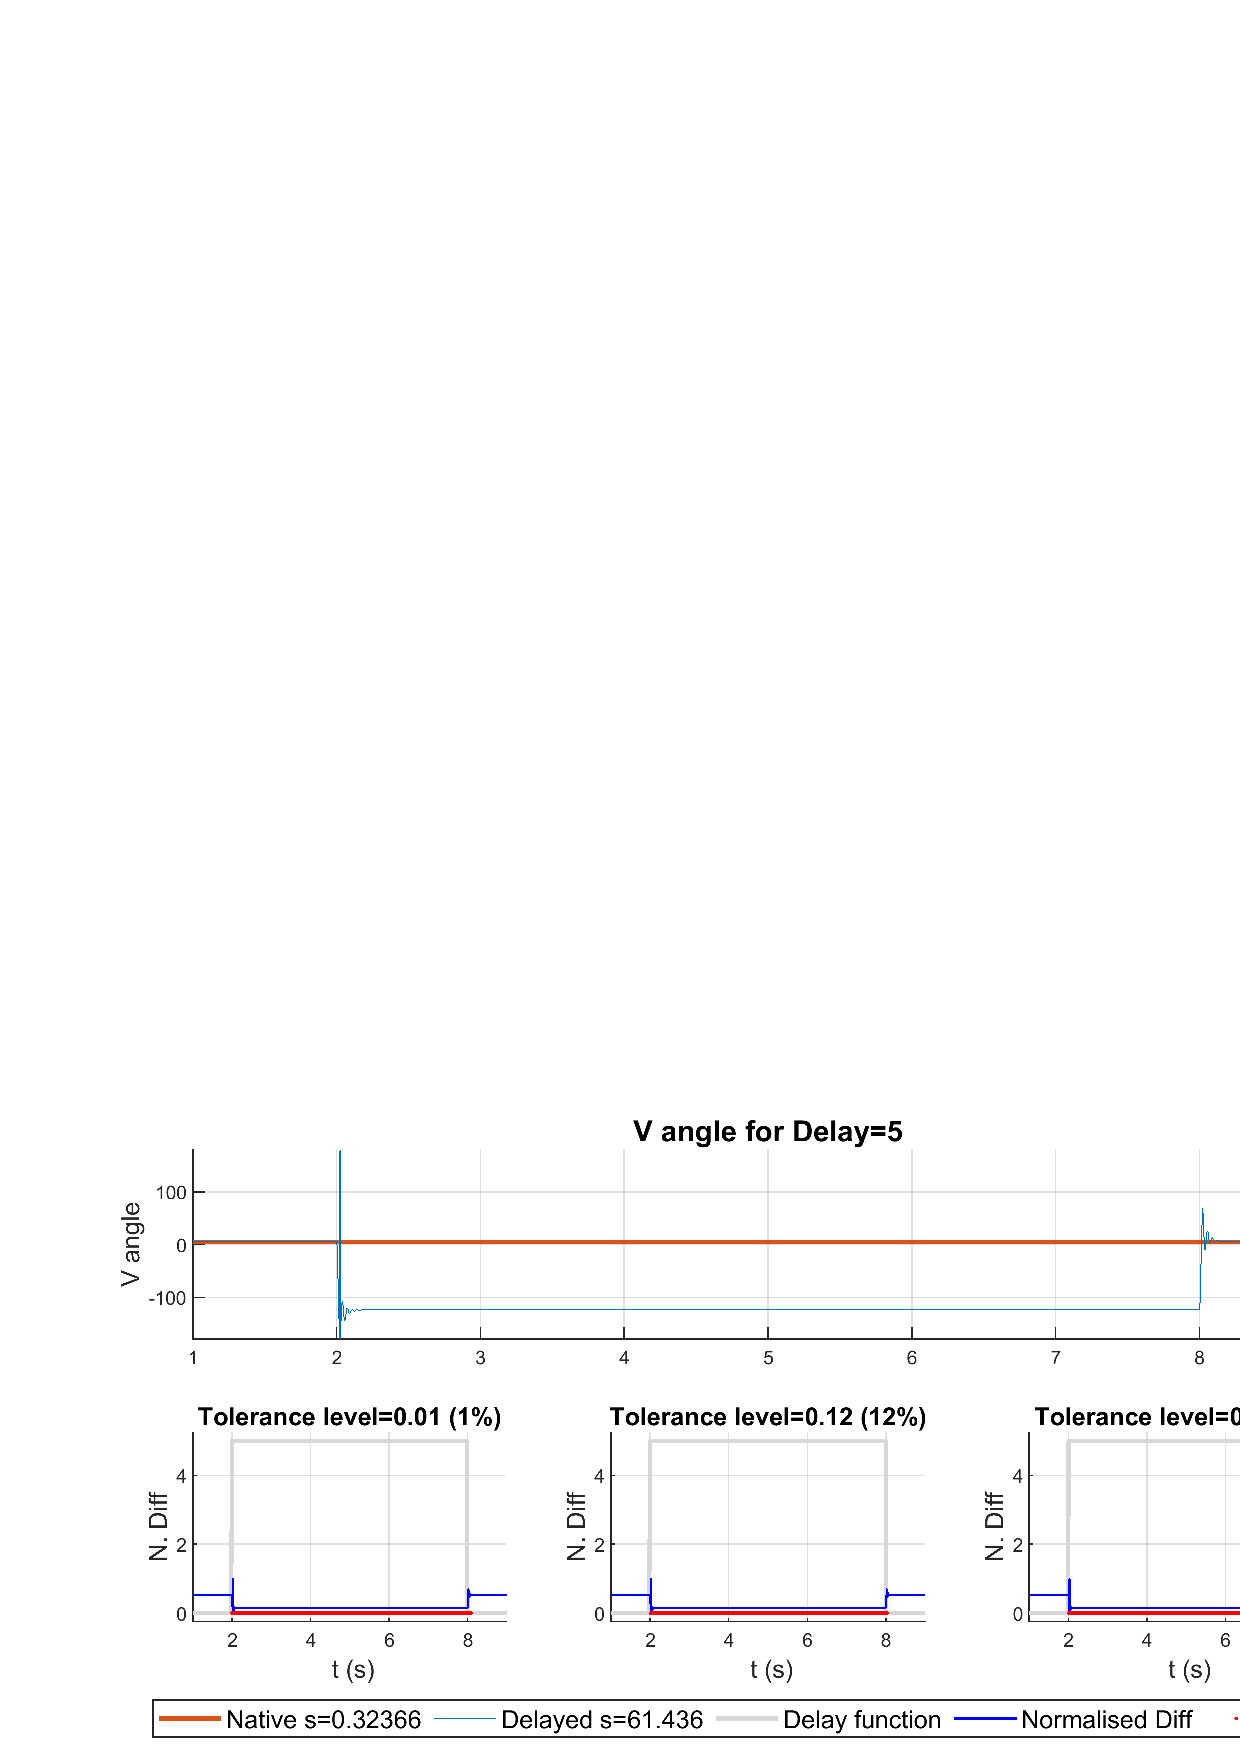
\includegraphics[width=0.95\textwidth]{PMUsim-figures/DelayOf_5/Instant_vAngle.png}} \\   
   \fbox{    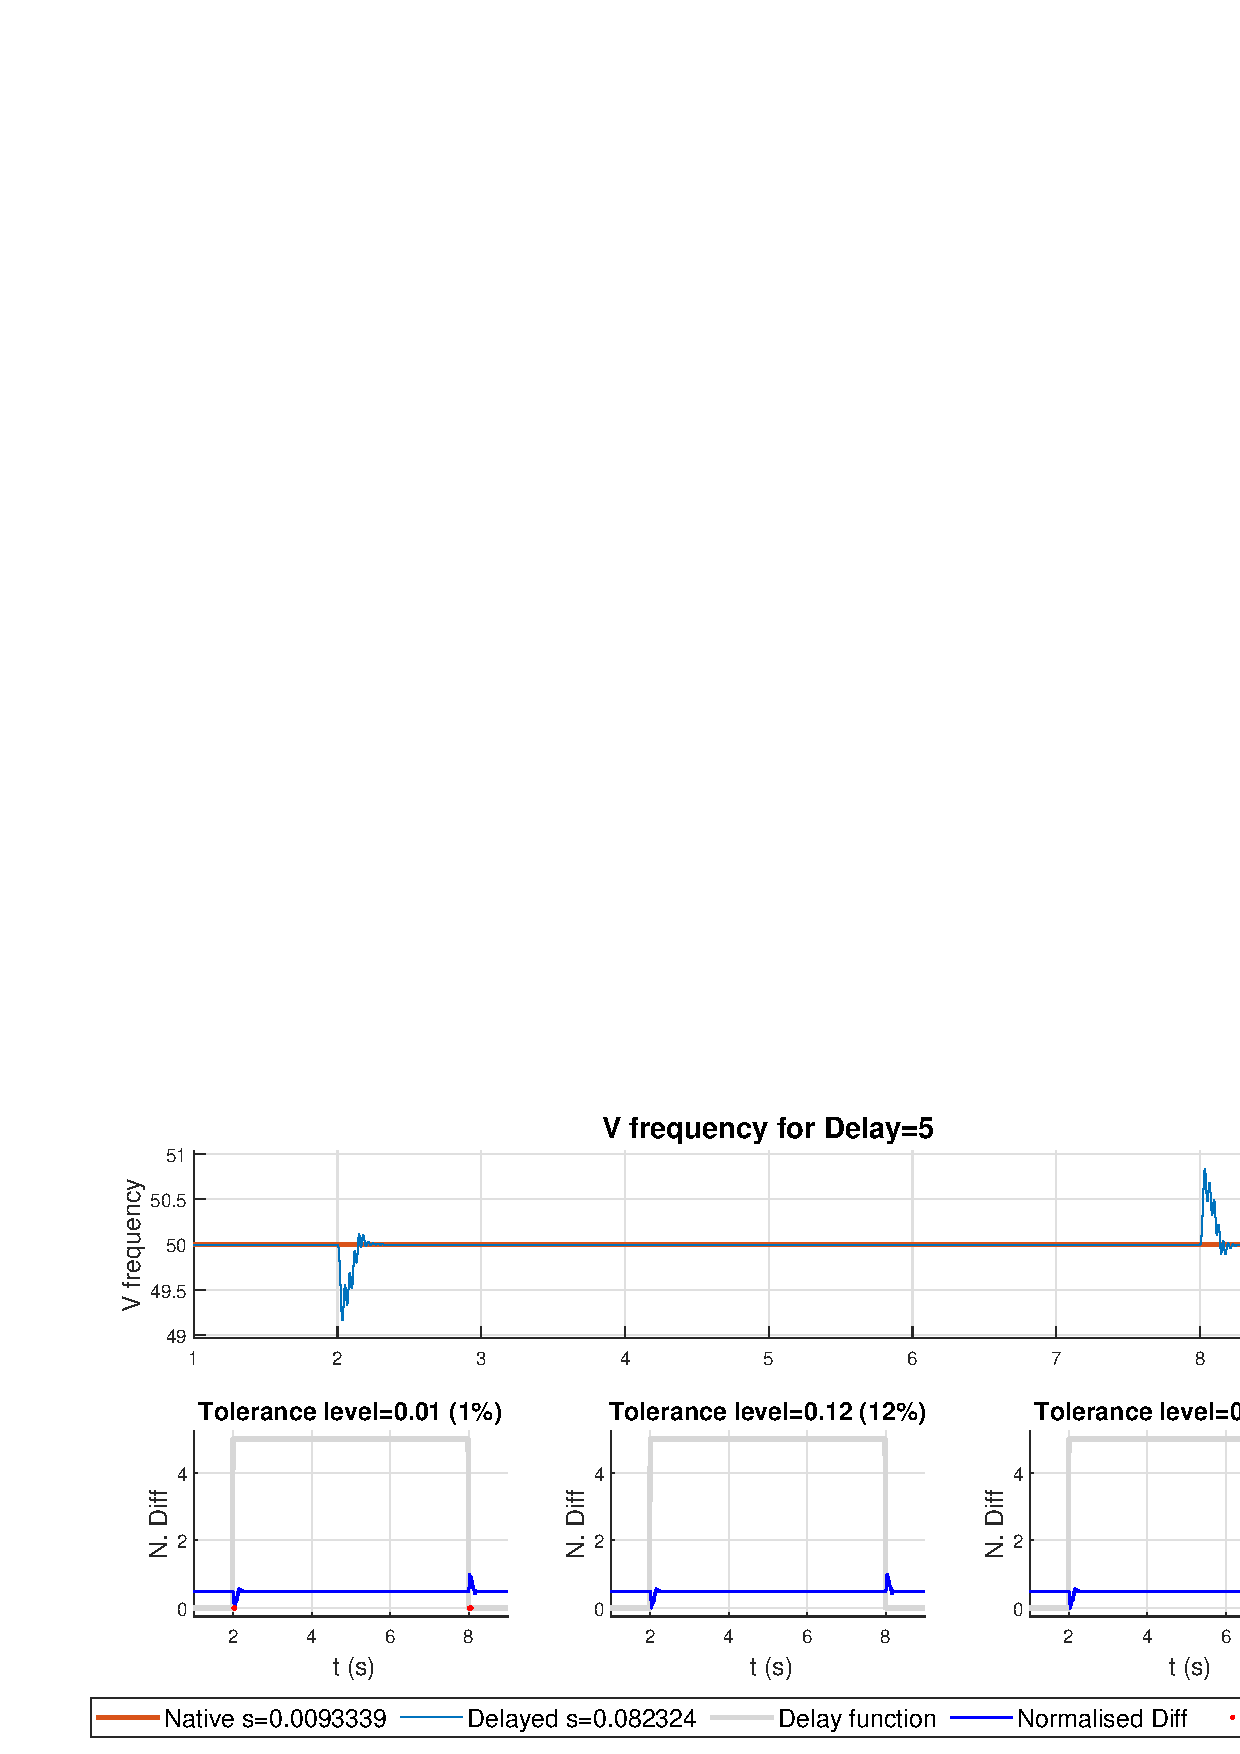
\includegraphics[width=0.95\textwidth]{PMUsim-figures/DelayOf_5/Instant_vFrequency.png}}


  \end{tabular}
\label{fig:VoltageInstantDelayFive}
\caption{Results for Voltage Output for Instant Delay equal to Five }
\end{figure}
\newpage
\begin{figure}[H]
\begin{tabular}{c}
  \fbox{  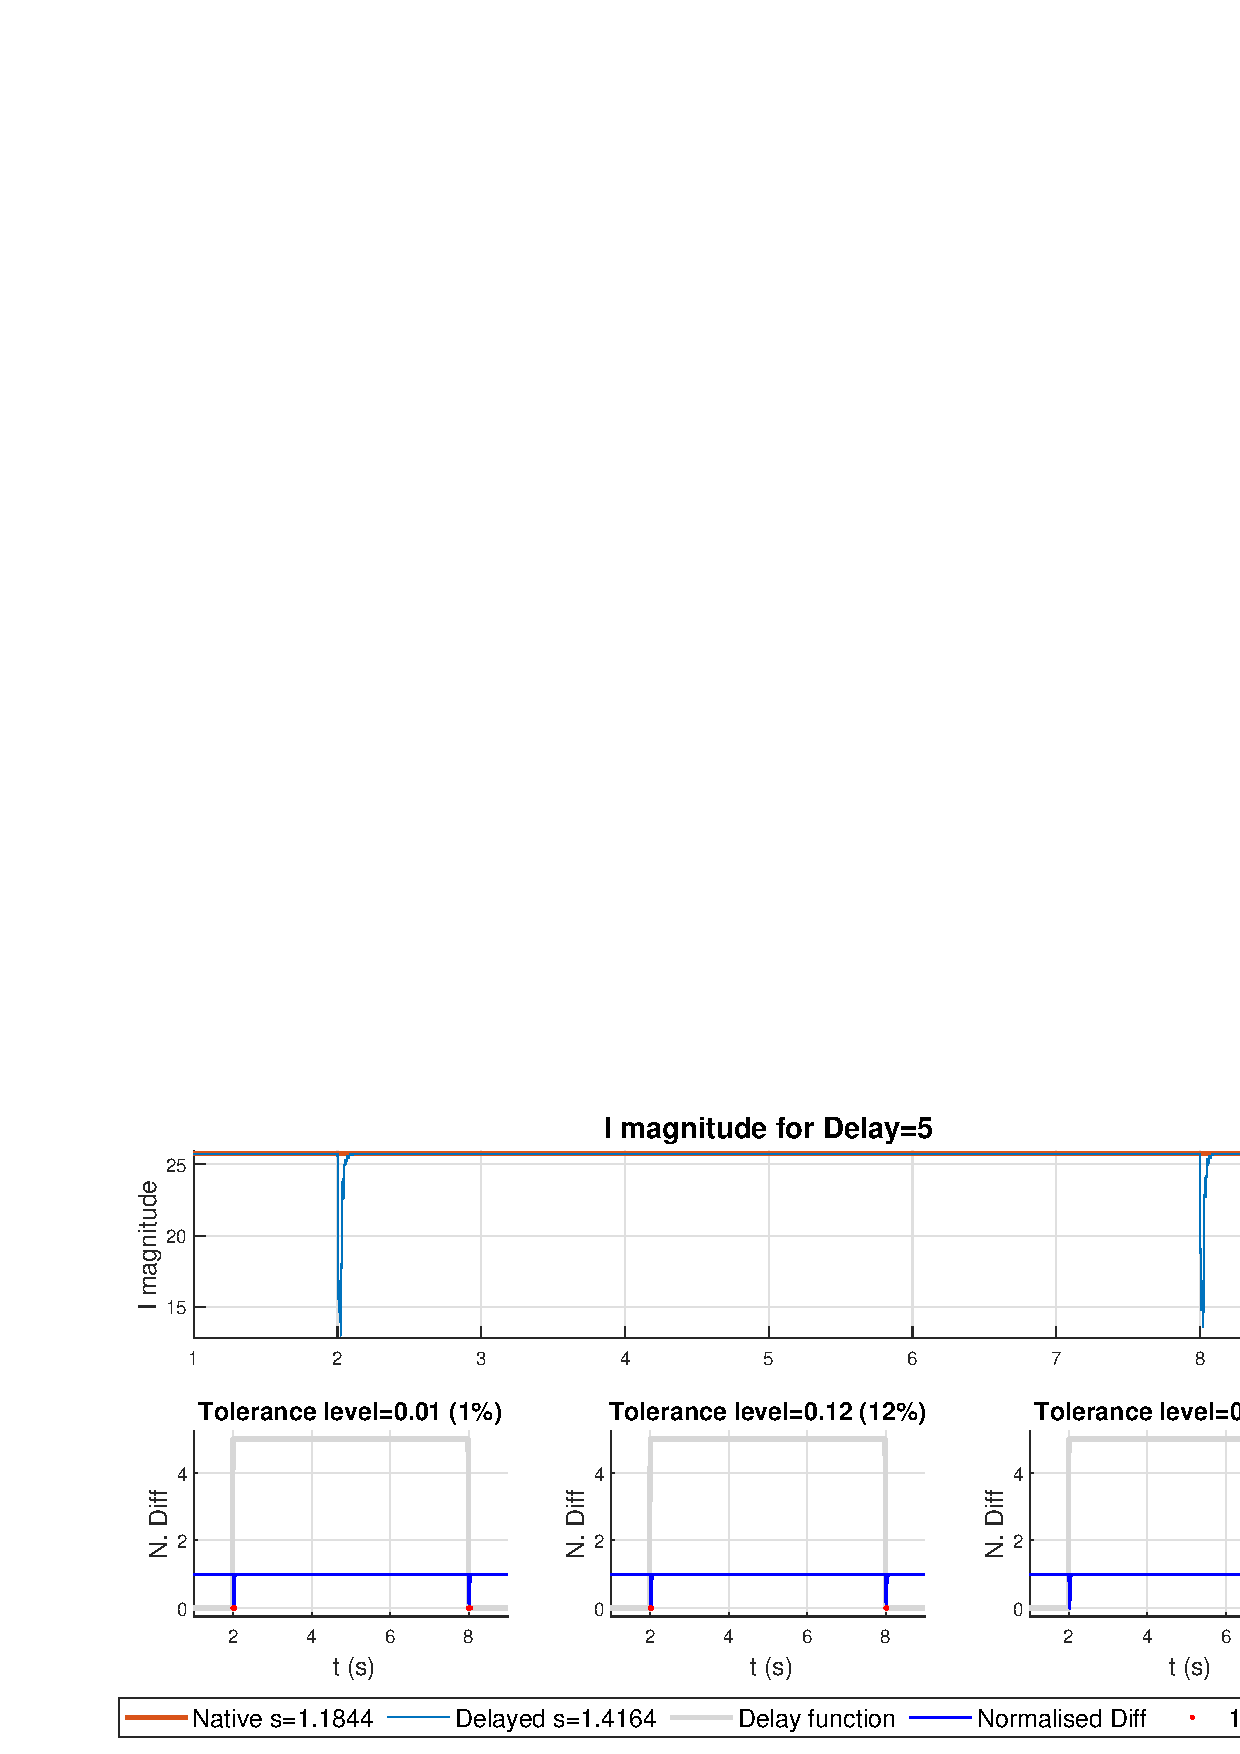
\includegraphics[width=0.95\textwidth]{PMUsim-figures/DelayOf_5/Instant_iMagnitude.png}} \\ 
    \fbox{     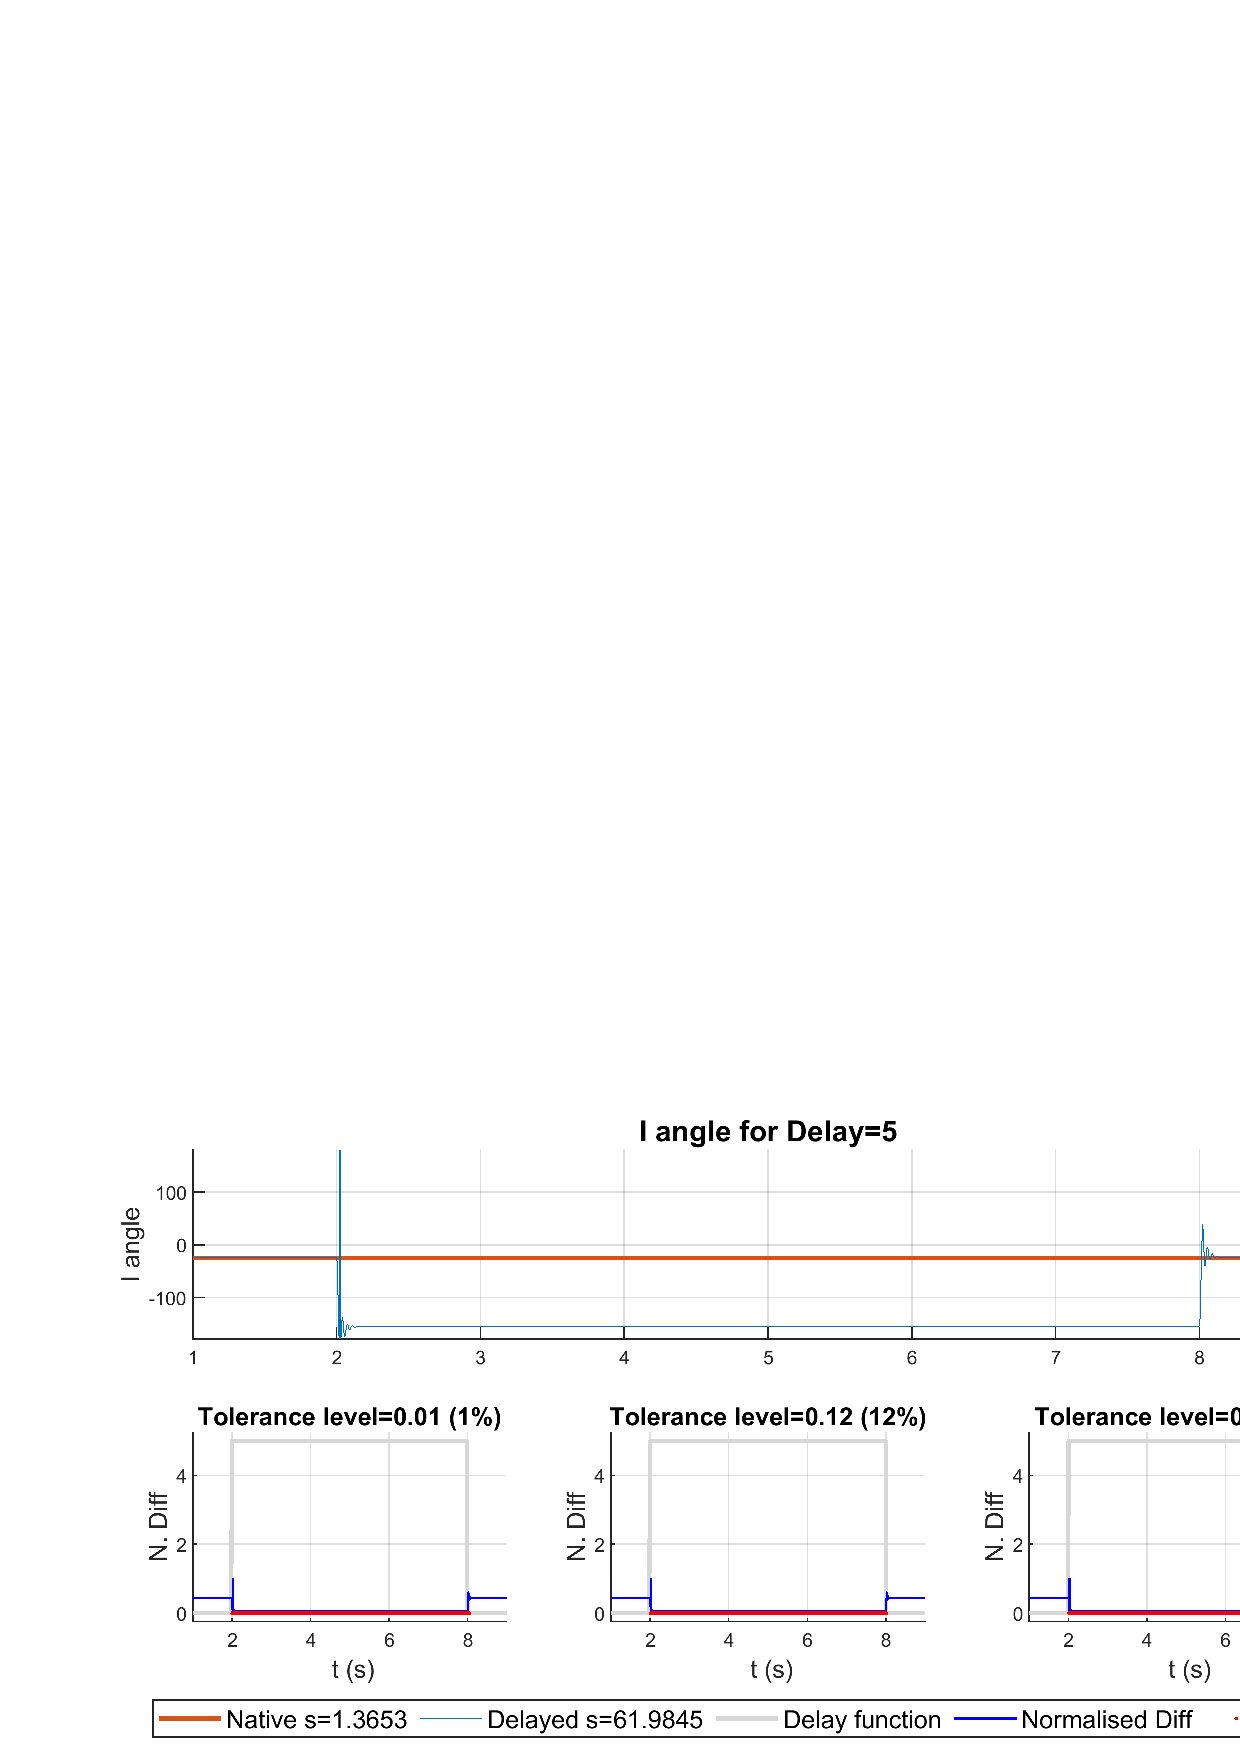
\includegraphics[width=0.95\textwidth]{PMUsim-figures/DelayOf_5/Instant_iAngle.png}} \\  
   \fbox{    \includegraphics[width=0.95\textwidth]{PMUsim-figures/DelayOf_5/Instant_iFrequency.png}}

 
  \end{tabular}
\label{fig:ImpedanceInstantDelayFive}
\caption{Results for Impedance Output for Instant Delay equal to Five }
\end{figure}


\newpage
\begin{figure}[H]
\begin{tabular}{c}
  \fbox{  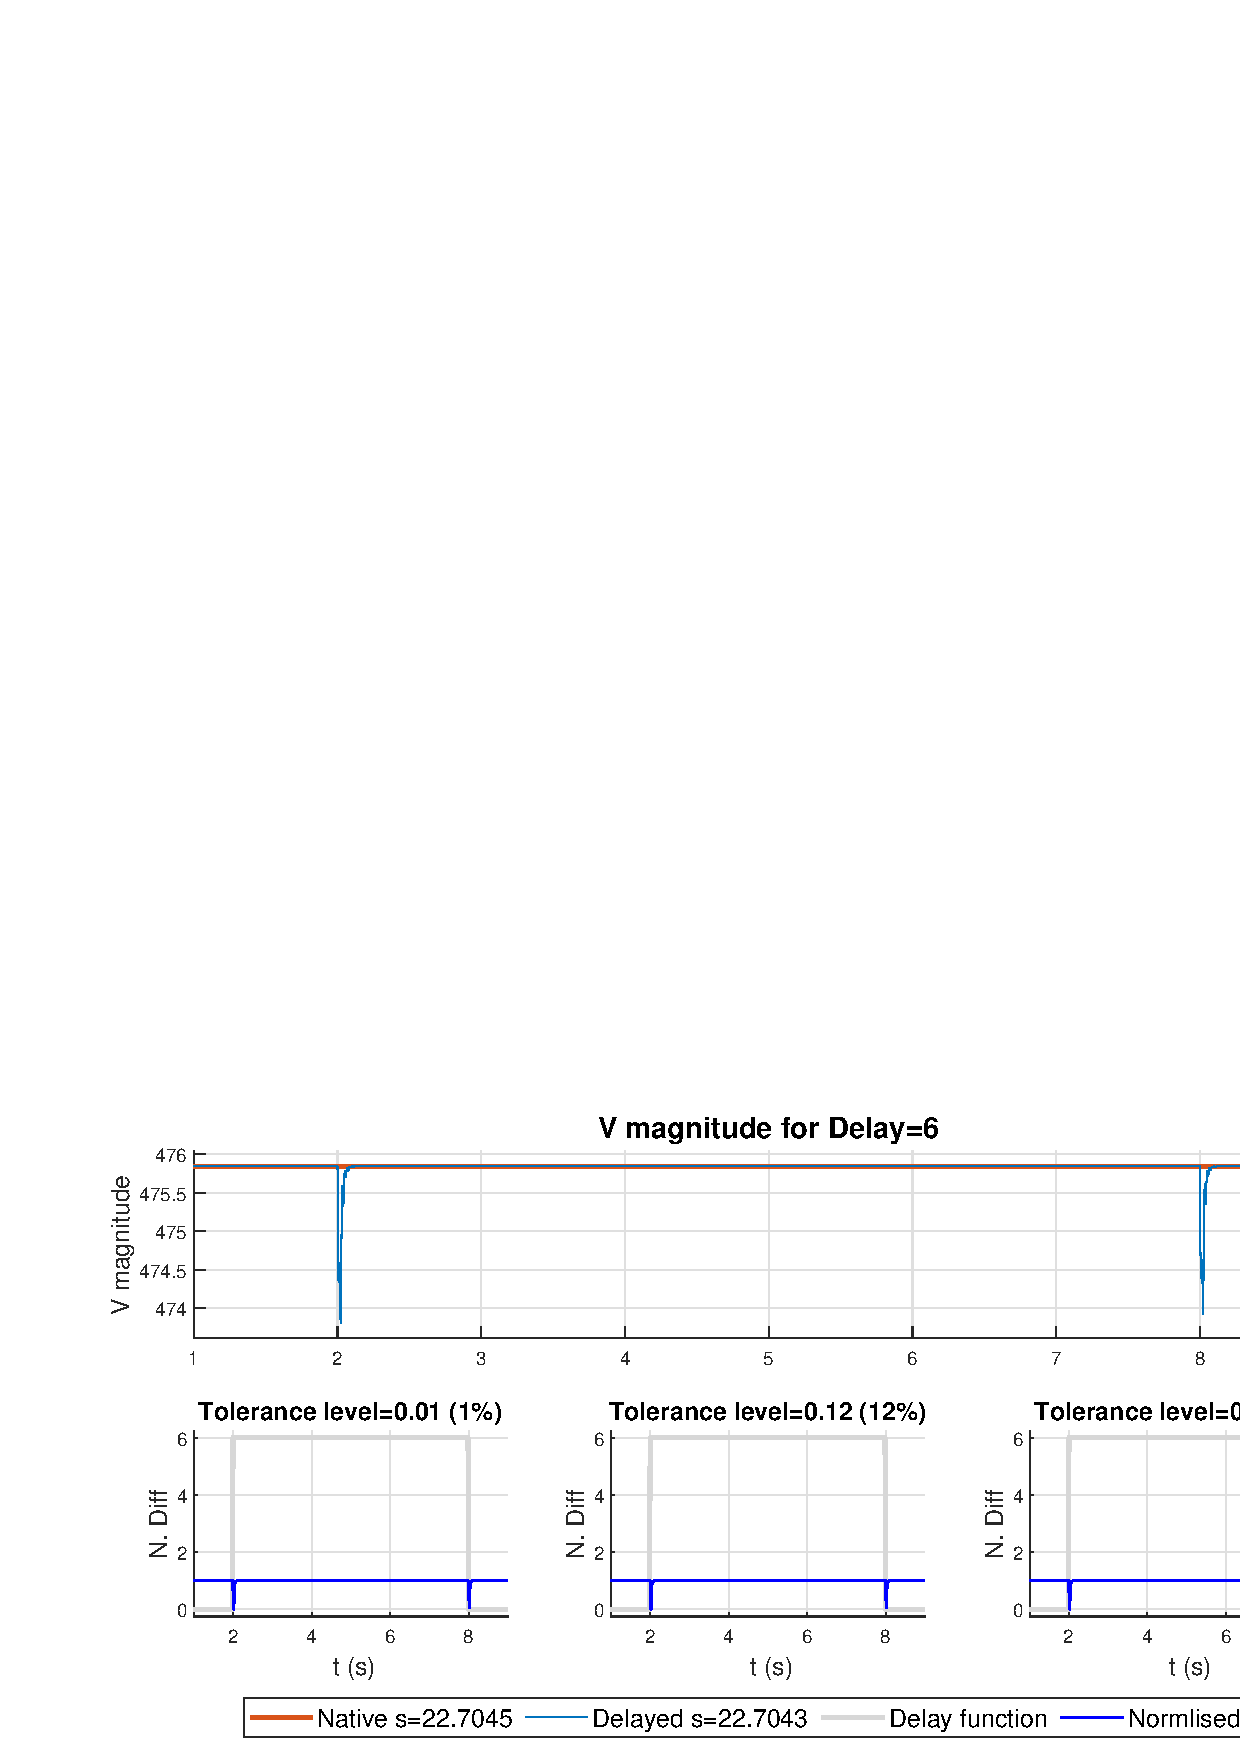
\includegraphics[width=0.95\textwidth]{PMUsim-figures/DelayOf_6/Instant_vMagnitude.png}} \\ 
   \fbox{     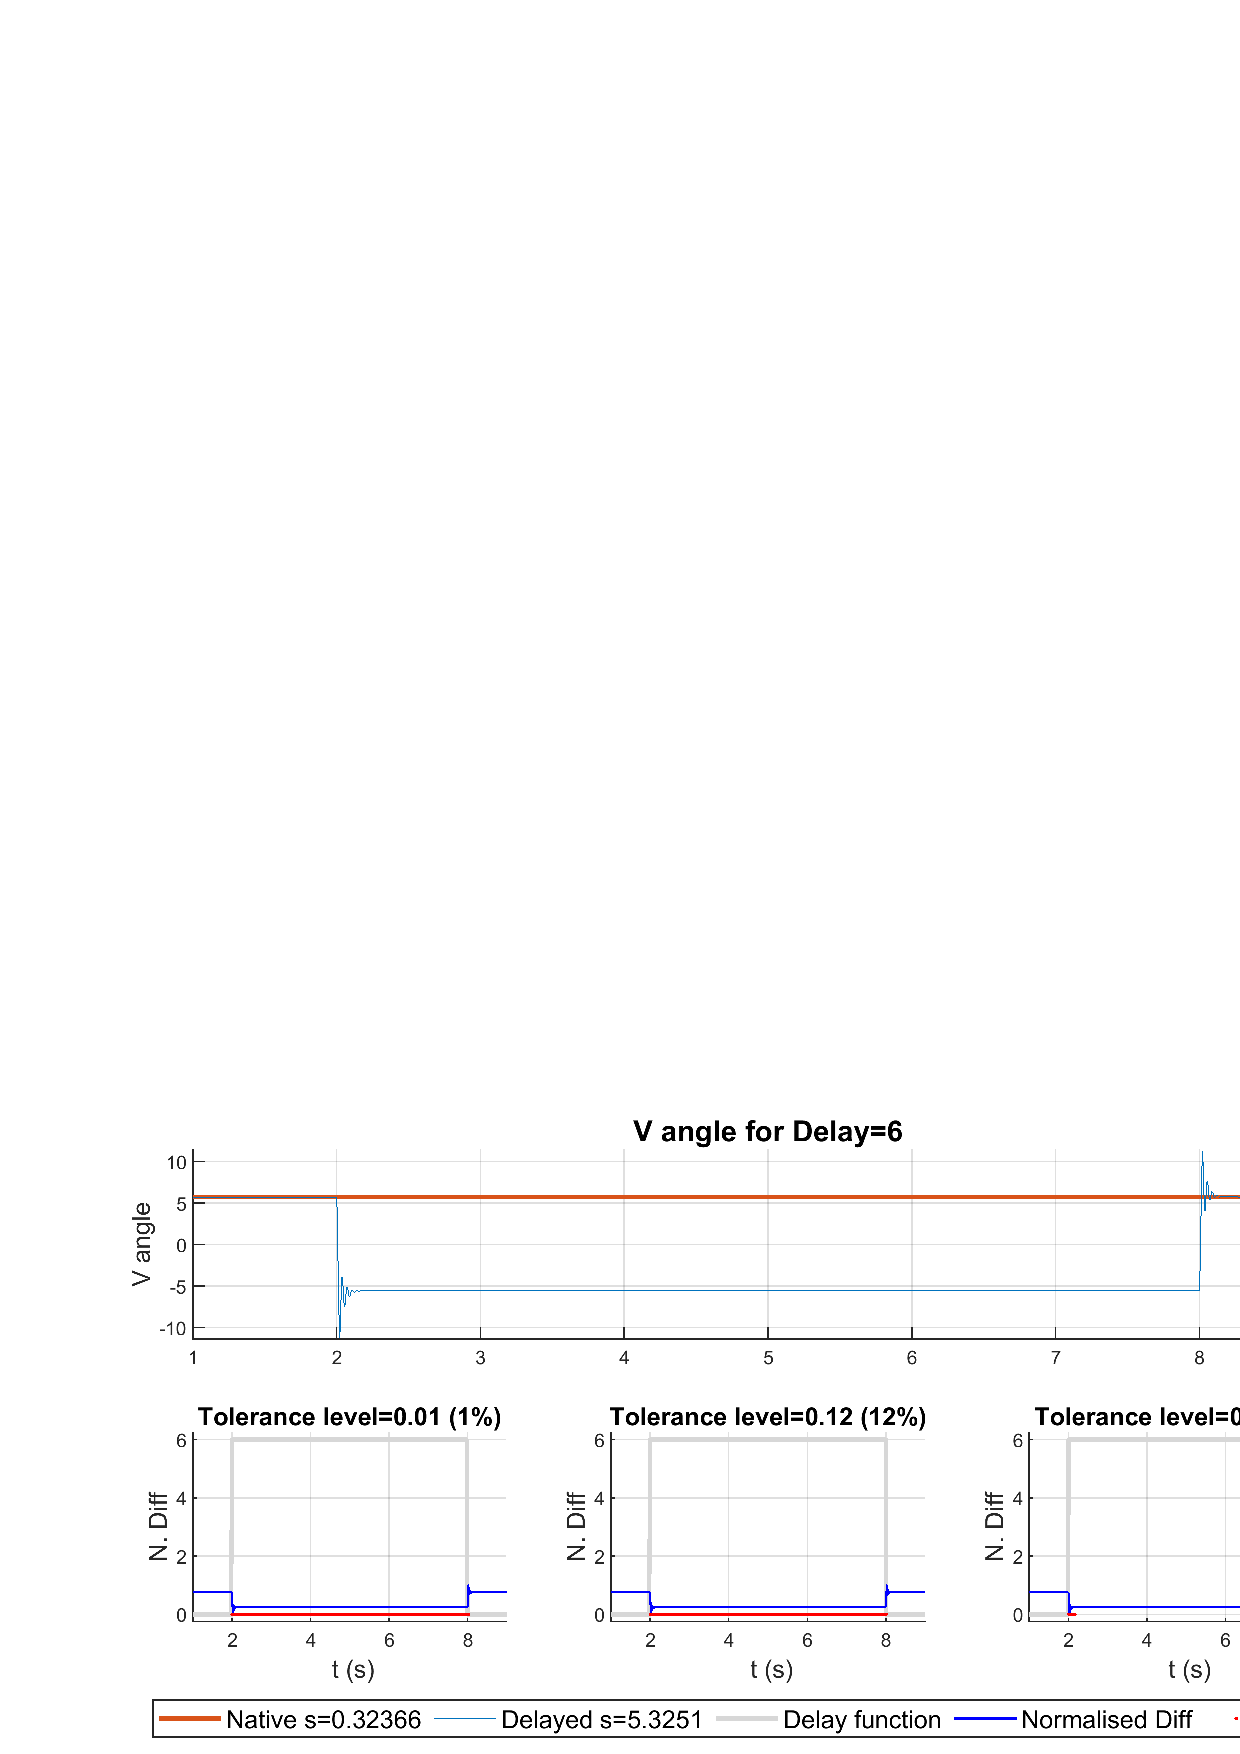
\includegraphics[width=0.95\textwidth]{PMUsim-figures/DelayOf_6/Instant_vAngle.png}} \\   
   \fbox{    \includegraphics[width=0.95\textwidth]{PMUsim-figures/DelayOf_6/Instant_vFrequency.png}}

 
  \end{tabular}
\label{fig:VoltageInstantDelaySix}
\caption{Results for Voltage Output for Instant Delay equal to Six }
\end{figure}
\newpage
\begin{figure}[H]
\begin{tabular}{c}
  \fbox{  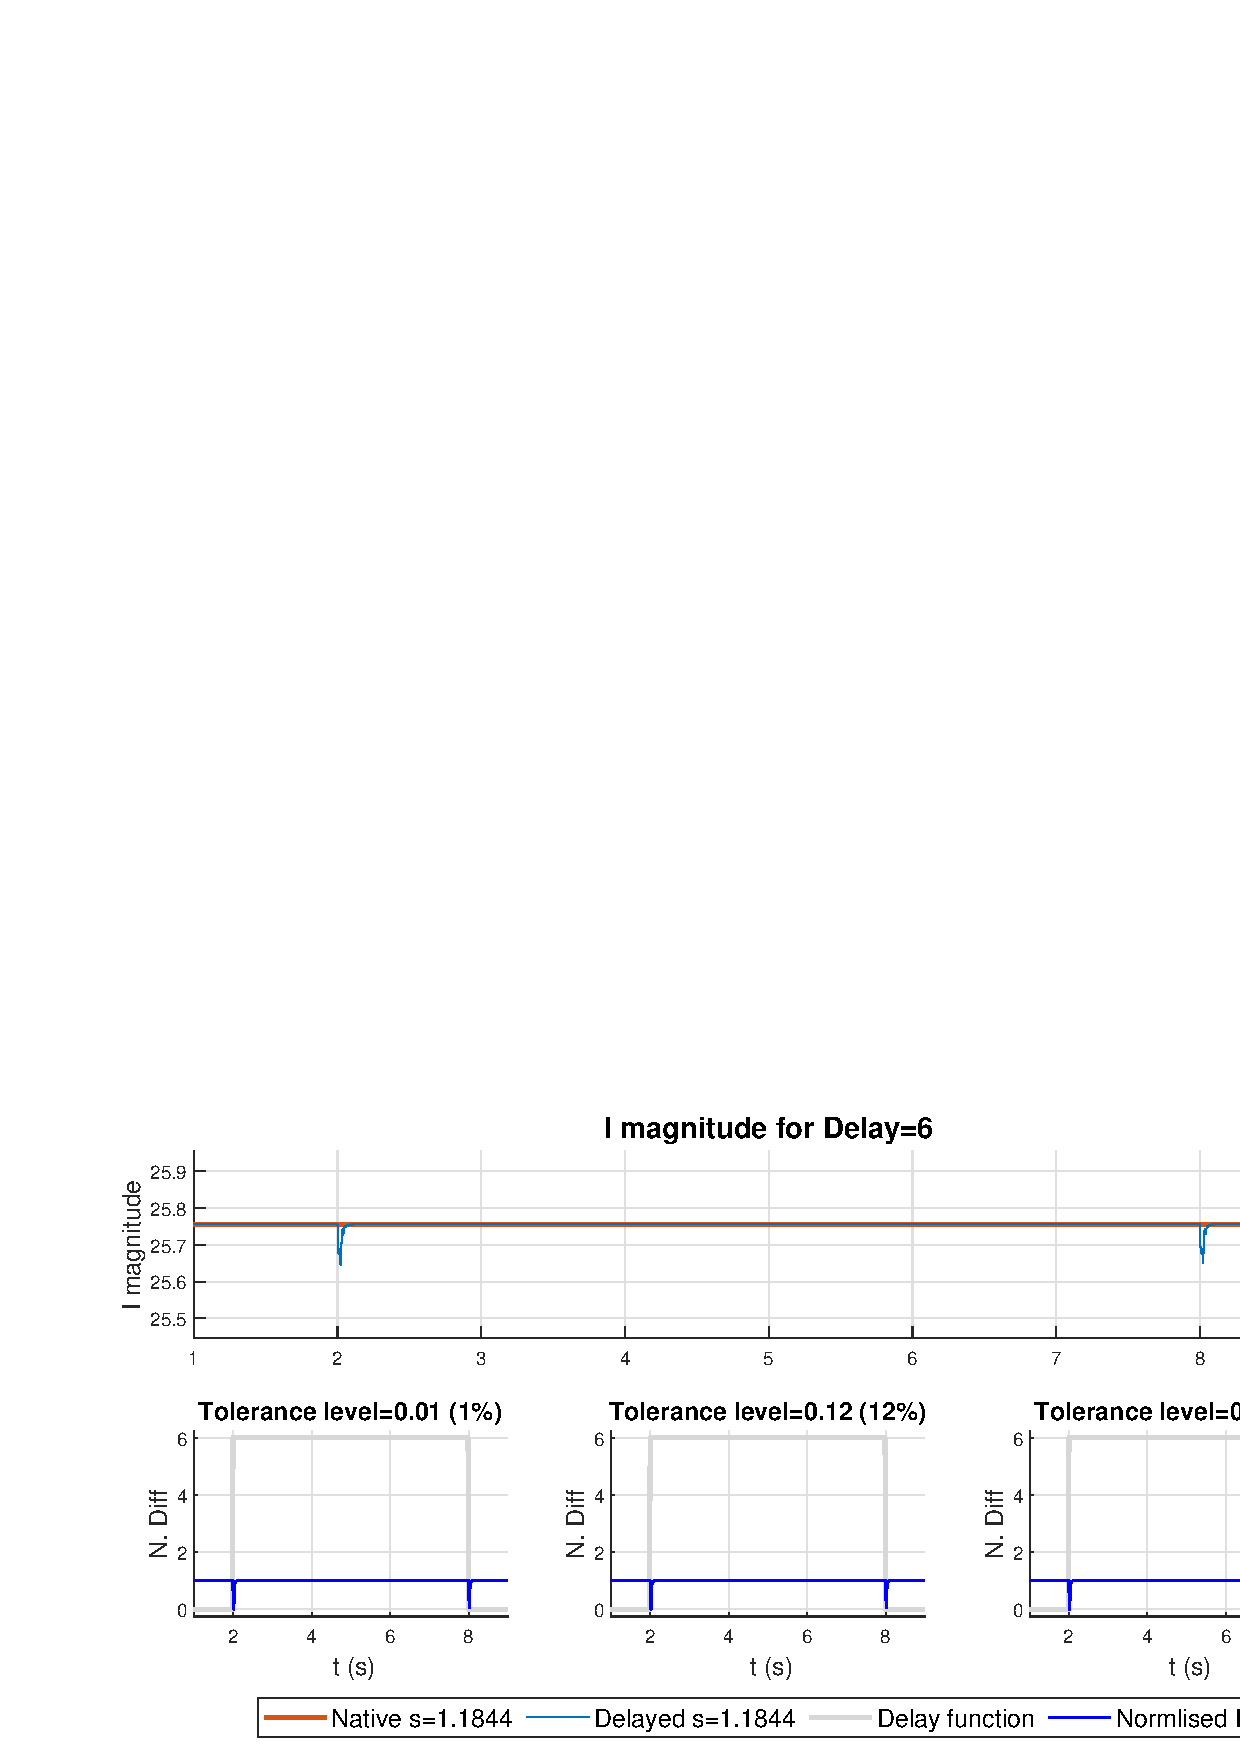
\includegraphics[width=0.95\textwidth]{PMUsim-figures/DelayOf_6/Instant_iMagnitude.png}} \\ 
   \fbox{     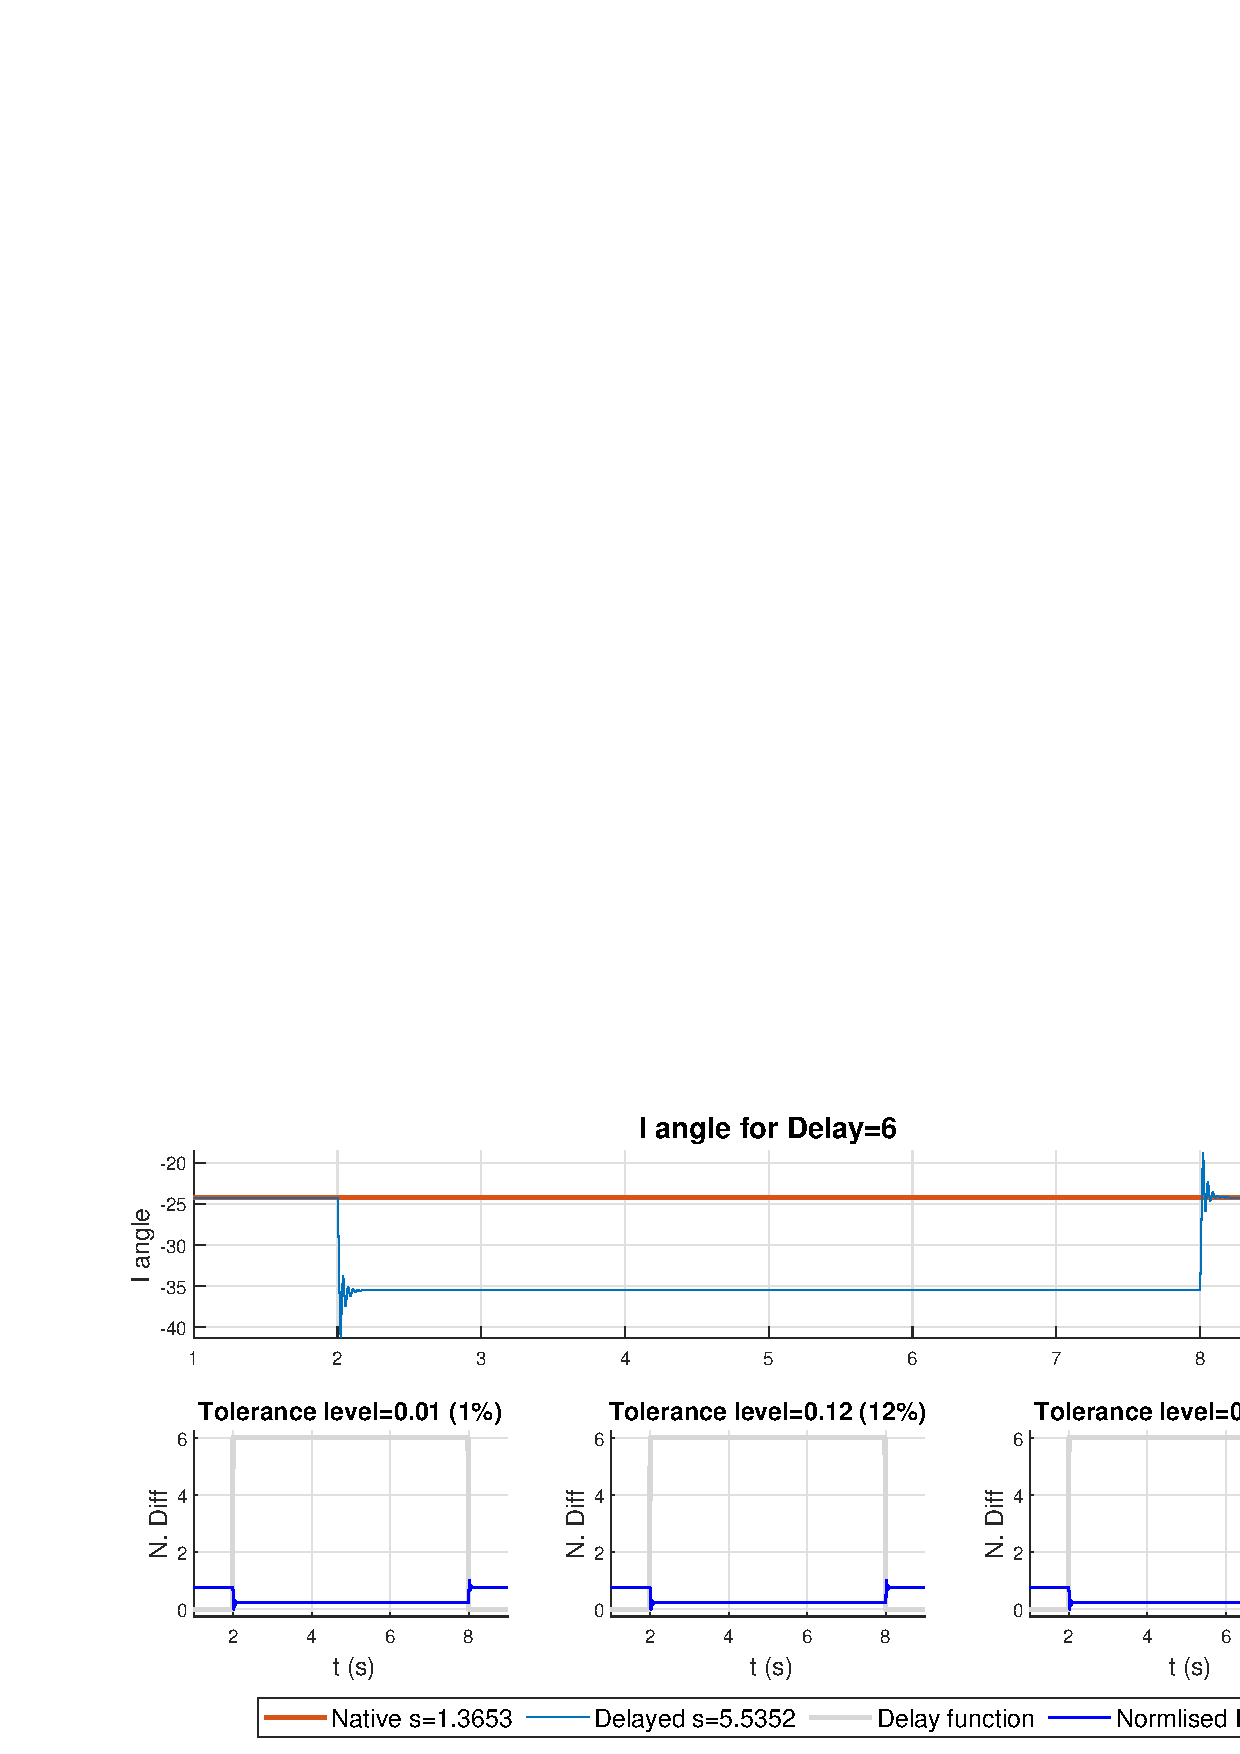
\includegraphics[width=0.95\textwidth]{PMUsim-figures/DelayOf_6/Instant_iAngle.png}} \\   
   \fbox{    \includegraphics[width=0.95\textwidth]{PMUsim-figures/DelayOf_6/Instant_iFrequency.png}}

 
  \end{tabular}
\label{fig:ImpedanceInstantDelaySix}
\caption{Results for Impedance Output for Instant Delay equal to Six }
\end{figure}

\newpage
\subsection{Conclusive remarks on instant delay simulations}


\subsubsection{Instant Delay Level of One}
Figures \ref{fig:VoltageInstantDelayOne} and \ref{fig:ImpedanceInstantDelayOne} shows the result of the Instant delay attack of level One. 

\subsubsection{Instant Delay Level of Two}
Figures \ref{fig:VoltageInstantDelayTwo} and \ref{fig:ImpedanceInstantDelayTwo} shows the result of the Instant delay attack of level Two. 

\subsubsection{Instant Delay Level of Three}
Figures \ref{fig:VoltageInstantDelayThree} and \ref{fig:ImpedanceInstantDelayThree} shows the result of the Instant delay attack of level Three. 

\subsubsection{Instant Delay Level of Four}
Figures \ref{fig:VoltageInstantDelayFour} and \ref{fig:ImpedanceInstantDelayFour} shows the result of the Instant delay attack of level Four. 

\subsubsection{Instant Delay Level of Five}
Figures \ref{fig:VoltageInstantDelayFive} and \ref{fig:ImpedanceInstantDelayFive} shows the result of the Instant delay attack of level Five. 

\subsubsection{Instant Delay Level of Six}
Figures \ref{fig:VoltageInstantDelaySix} and \ref{fig:ImpedanceInstantDelaySix} shows the result of the Instant delay attack of level Six. 








\newpage
\section{Step-Wise Delay functions}
The other flavour of delay attack considered, the step-Wise delay attack, focuses on effects caused by a slower rise of the delay level towards a pre-determined target level of delay. As there are no step-wise attack for delay level one, this category of attacks initiates the sequence of attacks by starting with a delay level of two.

The attack focuses on the following 
\begin{itemize}
\item What are the effects of repetitive increases of the delay level by one for different number of repetitions?
\item Are there any patterns observable:
\begin{itemize}
    \item Do the termination of the attack cancel the effect of the attack
    \item Do the next level of increase produce corresponding effects? 
\end{itemize}

\end{itemize}

















\newpage
\begin{figure}[H]
\begin{tabular}{c}
  \fbox{  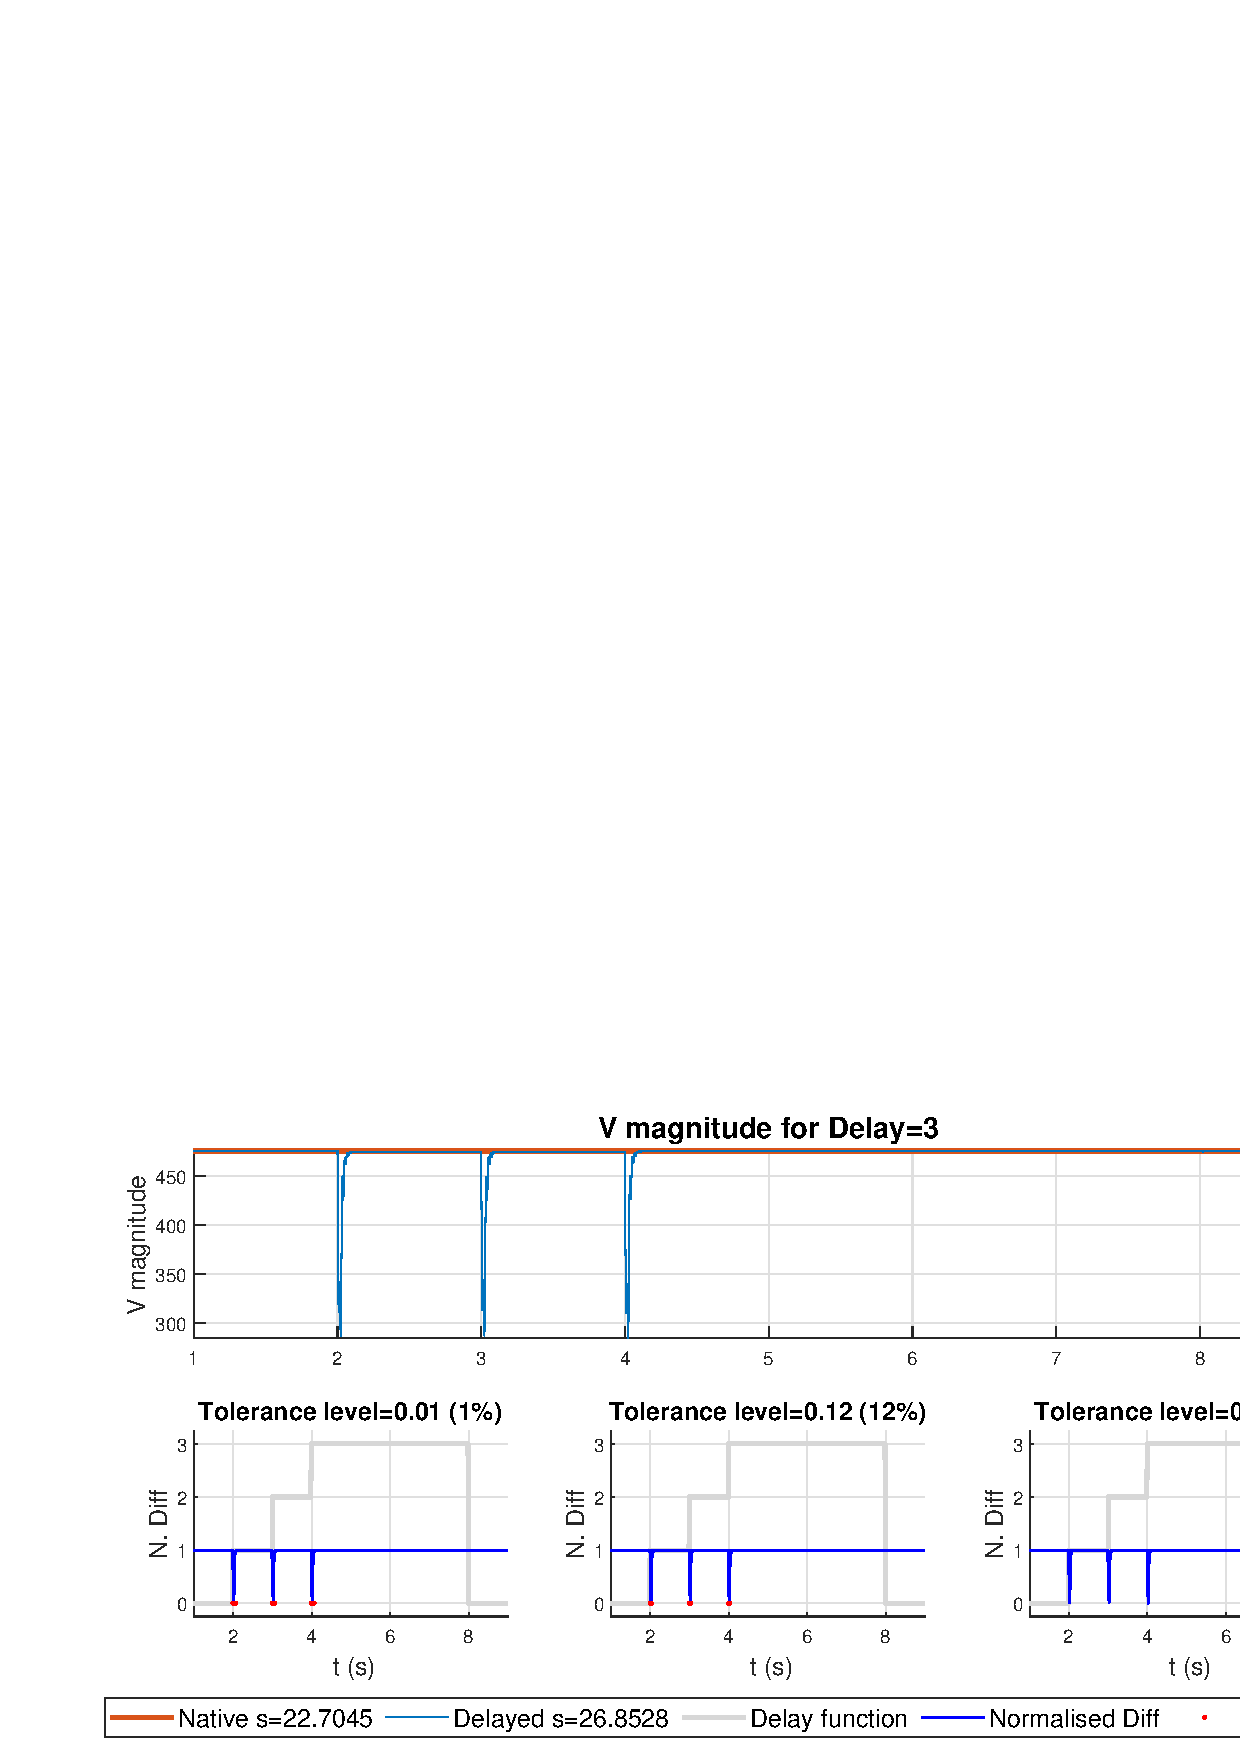
\includegraphics[width=0.95\textwidth]{PMUsim-figures/DelayOf_2/Step_vMagnitude.png}} \\ 
    \fbox{     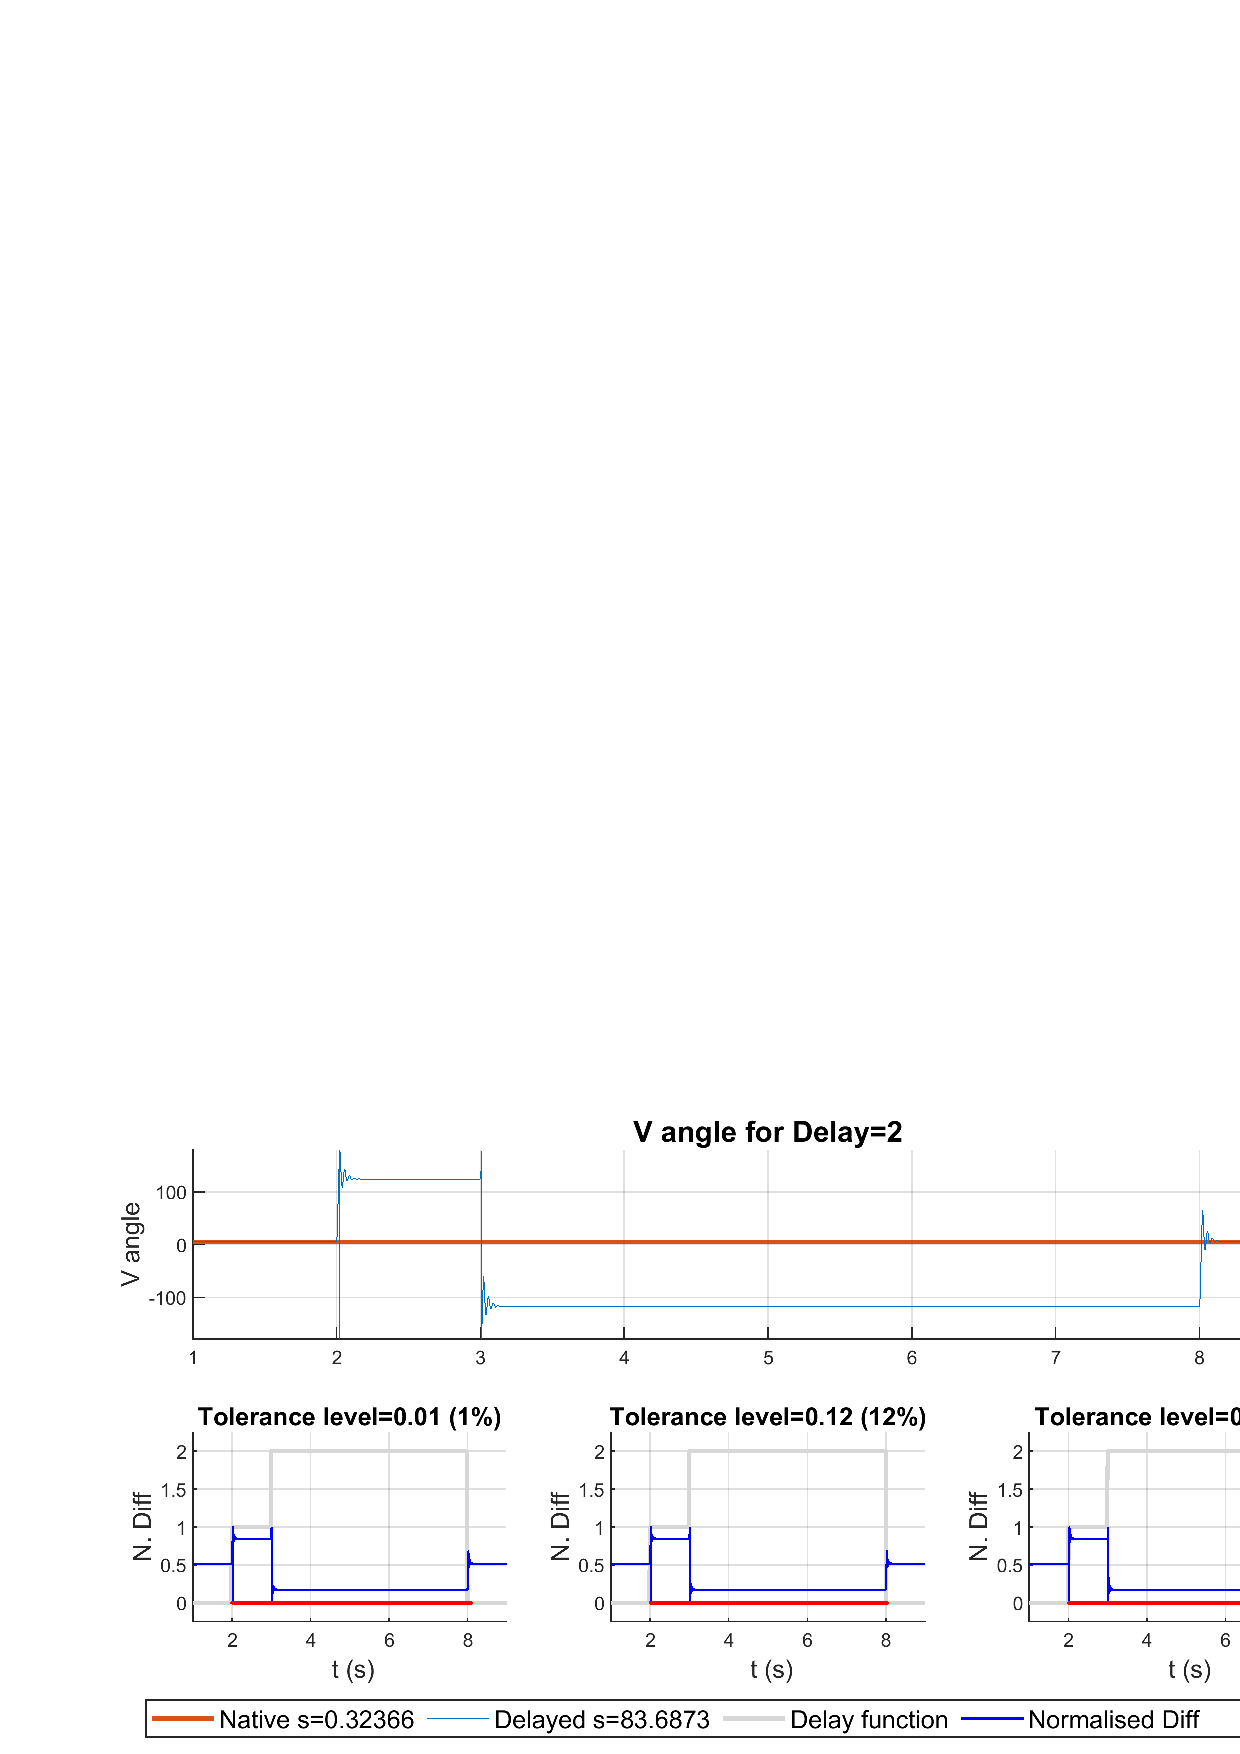
\includegraphics[width=0.95\textwidth]{PMUsim-figures/DelayOf_2/Step_vAngle.png}} \\ 
  
   \fbox{    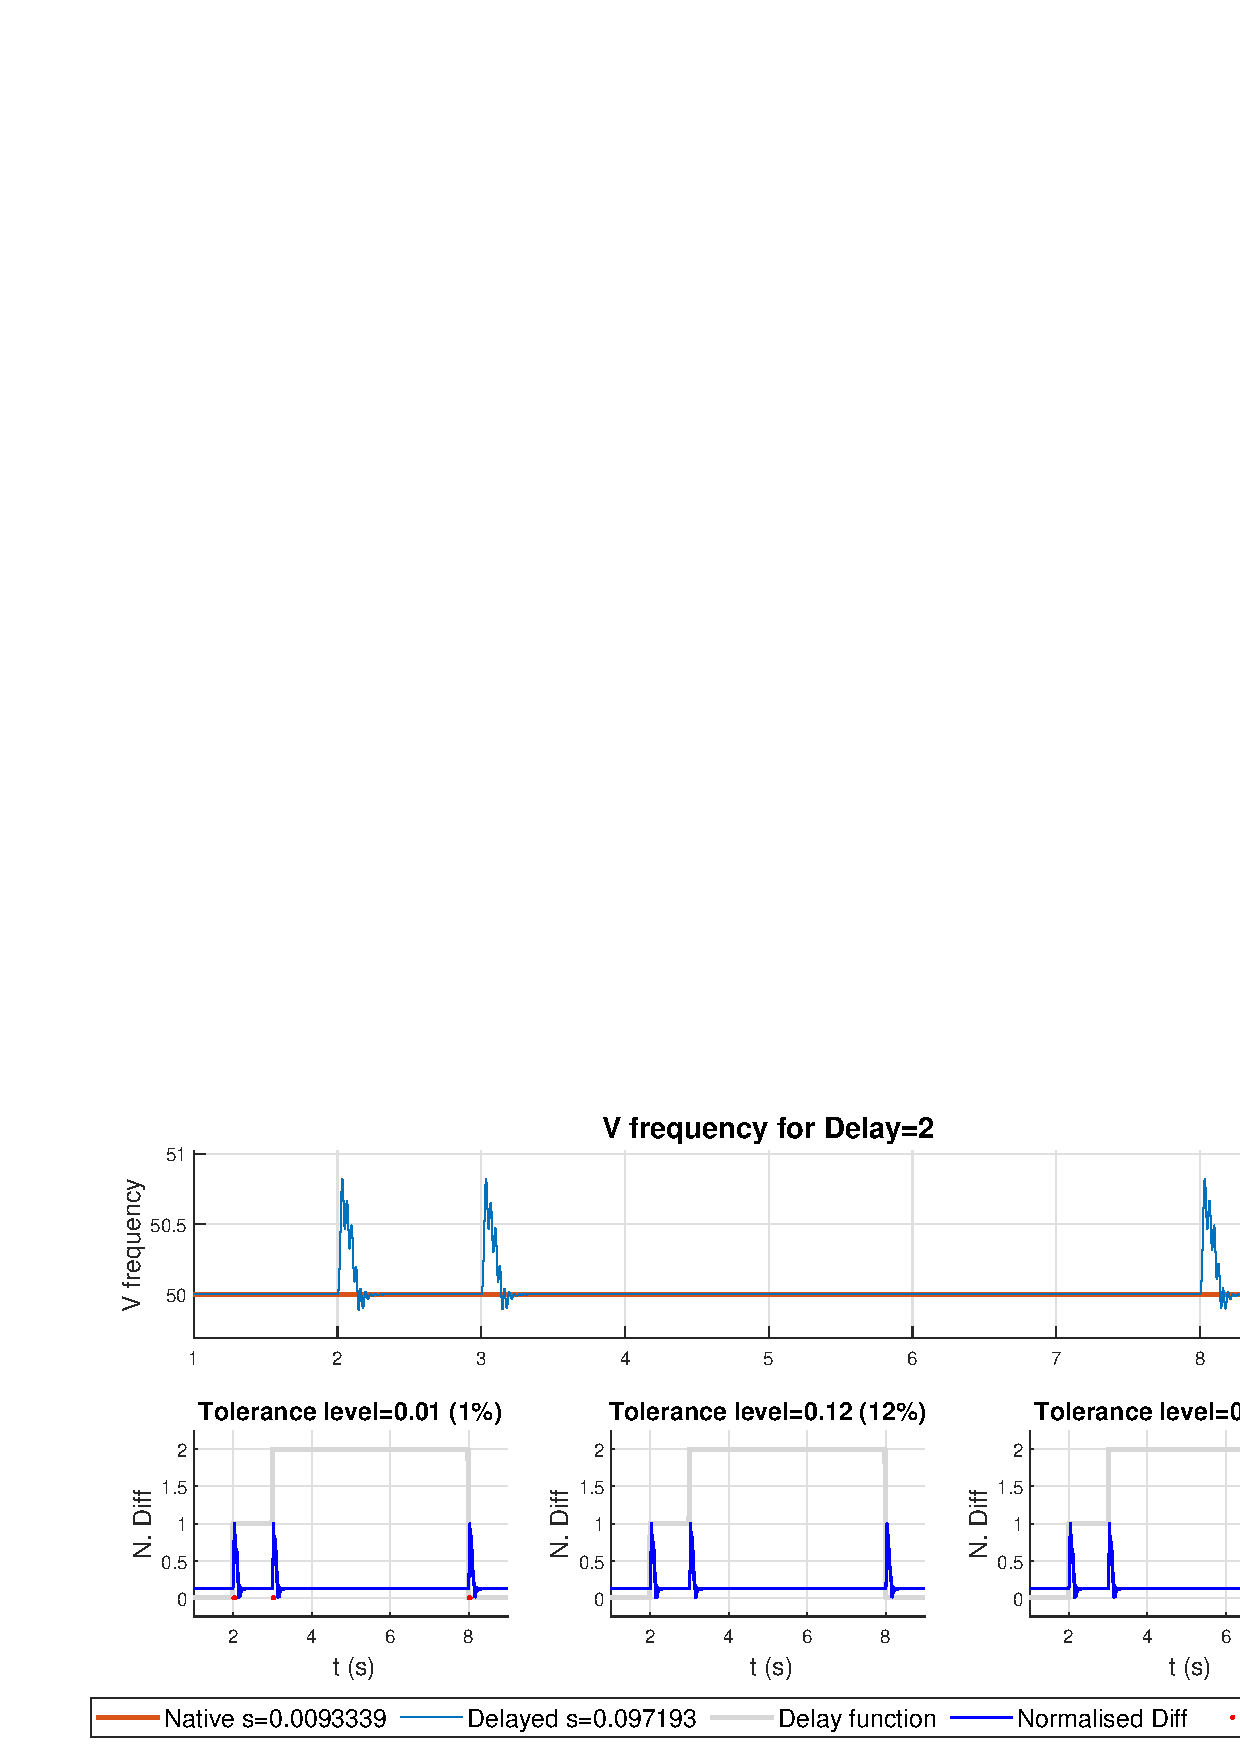
\includegraphics[width=0.95\textwidth]{PMUsim-figures/DelayOf_2/Step_vFrequency.png}}


  \end{tabular}
\label{fig:VoltageStepWiseDelayTwo}
\caption{Results for Voltage Output for Step-Wise Delay equal to Two }
\end{figure}
\newpage
\begin{figure}[H]
\begin{tabular}{c}
  \fbox{  \includegraphics[width=0.95\textwidth]{PMUsim-figures/DelayOf_2/Step_iMagnitude.png}} \\ 
   \fbox{     \includegraphics[width=0.95\textwidth]{PMUsim-figures/DelayOf_2/Step_iAngle.png}} \\   
   \fbox{    \includegraphics[width=0.95\textwidth]{PMUsim-figures/DelayOf_2/Step_iFrequency.png}} 


  \end{tabular}
\label{fig:ImpedanceStepWiseDelayDelayTwo}
\caption{Results for Impedance Output for Step-Wise Delay equal to Two }
\end{figure}





\newpage
\begin{figure}[H]
\begin{tabular}{c}
  \fbox{  \includegraphics[width=0.95\textwidth]{PMUsim-figures/DelayOf_3/Step_vMagnitude.png}} \\ 
   \fbox{     \includegraphics[width=0.95\textwidth]{PMUsim-figures/DelayOf_3/Step_vAngle.png}} \\    
   \fbox{    \includegraphics[width=0.95\textwidth]{PMUsim-figures/DelayOf_3/Step_vFrequency.png}}

  \end{tabular}
\label{fig:VoltageStepWiseDelayThree}
\caption{Results for Voltage Output for Step-Wise Delay equal to Three }
\end{figure}
\newpage
\begin{figure}[H]
\begin{tabular}{c}
  \fbox{  \includegraphics[width=0.95\textwidth]{PMUsim-figures/DelayOf_3/Step_iMagnitude.png}} \\ 
   \fbox{     \includegraphics[width=0.95\textwidth]{PMUsim-figures/DelayOf_3/Step_iAngle.png}} \\  
   \fbox{    \includegraphics[width=0.95\textwidth]{PMUsim-figures/DelayOf_3/Step_iFrequency.png}}

    

  \end{tabular}
\label{fig:ImpedanceStepWiseDelayThree}
\caption{Results for Impedance Output for Step-Wise Delay equal to Three }
\end{figure}






\newpage
\begin{figure}[H]
\begin{tabular}{c}
  \fbox{  \includegraphics[width=0.95\textwidth]{PMUsim-figures/DelayOf_4/Step_vMagnitude.png}} \\ 
   \fbox{     \includegraphics[width=0.95\textwidth]{PMUsim-figures/DelayOf_4/Step_vAngle.png}} \\    
   \fbox{    \includegraphics[width=0.95\textwidth]{PMUsim-figures/DelayOf_4/Step_vFrequency.png}}


  \end{tabular}
\label{fig:VoltageStepWiseDelayFour}
\caption{Results for Voltage Output for Step-Wise Delay equal to Four }
\end{figure}
\newpage
\begin{figure}[H]
\begin{tabular}{c}
  \fbox{  \includegraphics[width=0.95\textwidth]{PMUsim-figures/DelayOf_4/Step_iMagnitude.png}} \\ 
    \fbox{     \includegraphics[width=0.95\textwidth]{PMUsim-figures/DelayOf_4/Step_iAngle.png}}  \\  
   \fbox{    \includegraphics[width=0.95\textwidth]{PMUsim-figures/DelayOf_4/Step_iFrequency.png}} 


  \end{tabular}
\label{fig:ImpedanceStepWiseDelayFour}
\caption{Results for Impedance Output for Step-Wise Delay equal to Four }
\end{figure}




\newpage
\begin{figure}[H]
\begin{tabular}{c}
  \fbox{  \includegraphics[width=0.95\textwidth]{PMUsim-figures/DelayOf_5/Step_vMagnitude.png}} \\ 
  \fbox{     \includegraphics[width=0.95\textwidth]{PMUsim-figures/DelayOf_5/Step_vAngle.png}} \\    
   \fbox{    \includegraphics[width=0.95\textwidth]{PMUsim-figures/DelayOf_5/Step_vFrequency.png}}

 
  \end{tabular}
\label{fig:VoltageStepWiseDelayFive}
\caption{Results for Voltage Output for Step-Wise Delay equal to Five }
\end{figure}

\newpage
\begin{figure}[H]
\begin{tabular}{c}
  \fbox{  \includegraphics[width=0.95\textwidth]{PMUsim-figures/DelayOf_5/Step_iMagnitude.png}} \\ 
    \fbox{     \includegraphics[width=0.95\textwidth]{PMUsim-figures/DelayOf_5/Step_iAngle.png}}\\ 
   \fbox{    \includegraphics[width=0.95\textwidth]{PMUsim-figures/DelayOf_5/Step_iFrequency.png}} 
  \end{tabular}
\label{fig:ImpedanceStepWiseDelayFive}
\caption{Results for Impedance Output for Step-Wise Delay equal to Five }
\end{figure}


\newpage
\begin{figure}[H]
\begin{tabular}{c}
  \fbox{  \includegraphics[width=0.95\textwidth]{PMUsim-figures/DelayOf_6/Step_vMagnitude.png}} \\ 
  \fbox{     \includegraphics[width=0.95\textwidth]{PMUsim-figures/DelayOf_6/Step_vAngle.png}} \\ 
      \fbox{    \includegraphics[width=0.95\textwidth]{PMUsim-figures/DelayOf_6/Step_vFrequency.png}} 

 
  \end{tabular}
\caption{Results for Voltage Output for Step-Wise Delay equal to Six }
  \begin{tabular}{p{2cm} p{\textwidth-2cm}}
   & \\
  \textbf{Component} & \textbf{Main Observations} \\
    & \\
      Magnitude  & Drop in level at times of delay increase, no drop at reset to 0. \\
     Angle  &  Periodic reduction of difference for delay levels 3 and 6. \\
                & Alternating +/- differences for each increase of one \\
Frequency &  Similar spikes at any time of delaly change, even from 6 to 0
  \end{tabular}\label{fig:VoltageStepWiseDelayFSix}
\end{figure}

\newpage
\begin{figure}[H]
\begin{tabular}{c}
  \fbox{  \includegraphics[width=0.95\textwidth]{PMUsim-figures/DelayOf_6/Step_iMagnitude.png}} \\ 
    \fbox{     \includegraphics[width=0.95\textwidth]{PMUsim-figures/DelayOf_6/Step_iAngle.png}} \\
 
   \fbox{    \includegraphics[width=0.95\textwidth]{PMUsim-figures/DelayOf_6/Step_iFrequency.png}} 


  \end{tabular} 
\caption{Results for Impedance Output for Step-Wise Delay equal to Six}
  \begin{tabular}{p{2cm} p{\textwidth-2cm}}
   & \\
  \textbf{Component} & \textbf{Main Observations} \\
    & \\
      Magnitude  & Drop in level at times of delay increase, no drop at reset to 0. \\
     Angle  &  Periodic reduction of difference for delay levels 3 and 6. \\
                & Alternating +/- differences for each increase of one \\
Frequency &  Similar spikes at any time of delaly change, even from 6 to 0
  \end{tabular}
\label{fig:ImpedanceStepWiseDelayFSix}
\end{figure}


\newpage
\subsection{Conclusive remarks on running Step-Wise delay simulations}

\subsection{Step-Wise Delay Level of Two}
Figures \ref{fig:VoltageStepWiseDelayTwo} and \ref{fig:ImpedanceStepWiseDelayDelayTwo} shows the result of the Step-wise delay attack of level Two.
\subsection{Step-Wise Delay Level of Three}
Figures \ref{fig:VoltageStepWiseDelayThree} and \ref{fig:ImpedanceStepWiseDelayDelayThree} shows the result of the Step-wise delay attack of level Three.

\subsection{Step-Wise Delay Level of Four}
Figures \ref{fig:VoltageStepWiseDelayFour} and \ref{fig:ImpedanceStepWiseDelayDelayFour} shows the result of the Step-wise delay attack of level Four.

\subsection{Step-Wise Delay Level of Five}
Figures \ref{fig:VoltageStepWiseDelayFive} and \ref{fig:ImpedanceStepWiseDelayDelayFive} shows the result of the Step-wise delay attack of level Five.

\subsection{Step-Wise Delay Level of Six}
Figures \ref{fig:VoltageStepWiseDelaySix} and \ref{fig:ImpedanceStepWiseDelayDelaySix} shows the result of the Step-wise delay attack of level Six.





%\renewcommand{\locateResults}{PMUsim-figures/Ascending/DelayOf_1}
%\newpage
\section{Square pulse  delay function: Delay of 6}

\begin{figure}[hb]
 %   \includegraphics[trim=2 10 14 4, clip]{figures/v_AllFig-DelayOf_2-Sqaending.png}    
    \includegraphics[width=0.95\textwidth]{\locateResults/AllFig.png}    
    \caption{Square pulse  delay of 6: Combined output}
    \label{fig:PMUsim-Sqa6-allfig}
\end{figure}


     \begin{figure}
 
    \includegraphics[width=\textwidth]{\locateResults/Magnitude.png}    
         %\caption{Magnitude Output}
         \label{fig:PMUsim-Sqa6Mag}
        \caption{Square pulse  delay of 6: Magnitude component output}
 
\end{figure}

     \begin{figure}
 
   \includegraphics[width=\textwidth]{\locateResults/Angle.png}    
          %\caption{Angle Output}
         \label{fig:PMUsim-Sqa6Ang}
        \caption{Square pulse  delay of 6: Angle component output}
 
\end{figure}

     \begin{figure}
 
   \includegraphics[width=\textwidth]{\locateResults/Frequency.png}    
         %\caption{Frequency Output}
         \label{fig:PMUsim-Sqa6Freq}
        \caption{Square pulse  delay of 6: Frequency component output}
 
\end{figure}




%\renewcommand{\locateResults}{PMUsim-figures/Ascending/DelayOf_2}
%\newpage
\section{Square pulse  delay function: Delay of 6}

\begin{figure}[hb]
 %   \includegraphics[trim=2 10 14 4, clip]{figures/v_AllFig-DelayOf_2-Sqaending.png}    
    \includegraphics[width=0.95\textwidth]{\locateResults/AllFig.png}    
    \caption{Square pulse  delay of 6: Combined output}
    \label{fig:PMUsim-Sqa6-allfig}
\end{figure}


     \begin{figure}
 
    \includegraphics[width=\textwidth]{\locateResults/Magnitude.png}    
         %\caption{Magnitude Output}
         \label{fig:PMUsim-Sqa6Mag}
        \caption{Square pulse  delay of 6: Magnitude component output}
 
\end{figure}

     \begin{figure}
 
   \includegraphics[width=\textwidth]{\locateResults/Angle.png}    
          %\caption{Angle Output}
         \label{fig:PMUsim-Sqa6Ang}
        \caption{Square pulse  delay of 6: Angle component output}
 
\end{figure}

     \begin{figure}
 
   \includegraphics[width=\textwidth]{\locateResults/Frequency.png}    
         %\caption{Frequency Output}
         \label{fig:PMUsim-Sqa6Freq}
        \caption{Square pulse  delay of 6: Frequency component output}
 
\end{figure}




%\renewcommand{\locateResults}{PMUsim-figures/Cont/DelayOf_2}
%\newpage
\section{Square pulse  delay function: Delay of 6}

\begin{figure}[hb]
 %   \includegraphics[trim=2 10 14 4, clip]{figures/v_AllFig-DelayOf_2-Sqaending.png}    
    \includegraphics[width=0.95\textwidth]{\locateResults/AllFig.png}    
    \caption{Square pulse  delay of 6: Combined output}
    \label{fig:PMUsim-Sqa6-allfig}
\end{figure}


     \begin{figure}
 
    \includegraphics[width=\textwidth]{\locateResults/Magnitude.png}    
         %\caption{Magnitude Output}
         \label{fig:PMUsim-Sqa6Mag}
        \caption{Square pulse  delay of 6: Magnitude component output}
 
\end{figure}

     \begin{figure}
 
   \includegraphics[width=\textwidth]{\locateResults/Angle.png}    
          %\caption{Angle Output}
         \label{fig:PMUsim-Sqa6Ang}
        \caption{Square pulse  delay of 6: Angle component output}
 
\end{figure}

     \begin{figure}
 
   \includegraphics[width=\textwidth]{\locateResults/Frequency.png}    
         %\caption{Frequency Output}
         \label{fig:PMUsim-Sqa6Freq}
        \caption{Square pulse  delay of 6: Frequency component output}
 
\end{figure}




%\renewcommand{\locateResults}{PMUsim-figures/Square/DelayOf_2}
%\newpage
\section{Square pulse  delay function: Delay of 6}

\begin{figure}[hb]
 %   \includegraphics[trim=2 10 14 4, clip]{figures/v_AllFig-DelayOf_2-Sqaending.png}    
    \includegraphics[width=0.95\textwidth]{\locateResults/AllFig.png}    
    \caption{Square pulse  delay of 6: Combined output}
    \label{fig:PMUsim-Sqa6-allfig}
\end{figure}


     \begin{figure}
 
    \includegraphics[width=\textwidth]{\locateResults/Magnitude.png}    
         %\caption{Magnitude Output}
         \label{fig:PMUsim-Sqa6Mag}
        \caption{Square pulse  delay of 6: Magnitude component output}
 
\end{figure}

     \begin{figure}
 
   \includegraphics[width=\textwidth]{\locateResults/Angle.png}    
          %\caption{Angle Output}
         \label{fig:PMUsim-Sqa6Ang}
        \caption{Square pulse  delay of 6: Angle component output}
 
\end{figure}

     \begin{figure}
 
   \includegraphics[width=\textwidth]{\locateResults/Frequency.png}    
         %\caption{Frequency Output}
         \label{fig:PMUsim-Sqa6Freq}
        \caption{Square pulse  delay of 6: Frequency component output}
 
\end{figure}




%\renewcommand{\locateResults}{PMUsim-figures/Ascending/DelayOf_6}
%\newpage
\section{Square pulse  delay function: Delay of 6}

\begin{figure}[hb]
 %   \includegraphics[trim=2 10 14 4, clip]{figures/v_AllFig-DelayOf_2-Sqaending.png}    
    \includegraphics[width=0.95\textwidth]{\locateResults/AllFig.png}    
    \caption{Square pulse  delay of 6: Combined output}
    \label{fig:PMUsim-Sqa6-allfig}
\end{figure}


     \begin{figure}
 
    \includegraphics[width=\textwidth]{\locateResults/Magnitude.png}    
         %\caption{Magnitude Output}
         \label{fig:PMUsim-Sqa6Mag}
        \caption{Square pulse  delay of 6: Magnitude component output}
 
\end{figure}

     \begin{figure}
 
   \includegraphics[width=\textwidth]{\locateResults/Angle.png}    
          %\caption{Angle Output}
         \label{fig:PMUsim-Sqa6Ang}
        \caption{Square pulse  delay of 6: Angle component output}
 
\end{figure}

     \begin{figure}
 
   \includegraphics[width=\textwidth]{\locateResults/Frequency.png}    
         %\caption{Frequency Output}
         \label{fig:PMUsim-Sqa6Freq}
        \caption{Square pulse  delay of 6: Frequency component output}
 
\end{figure}




%\renewcommand{\locateResults}{PMUsim-figures/Cont/DelayOf_6}
%\newpage
\section{Square pulse  delay function: Delay of 6}

\begin{figure}[hb]
 %   \includegraphics[trim=2 10 14 4, clip]{figures/v_AllFig-DelayOf_2-Sqaending.png}    
    \includegraphics[width=0.95\textwidth]{\locateResults/AllFig.png}    
    \caption{Square pulse  delay of 6: Combined output}
    \label{fig:PMUsim-Sqa6-allfig}
\end{figure}


     \begin{figure}
 
    \includegraphics[width=\textwidth]{\locateResults/Magnitude.png}    
         %\caption{Magnitude Output}
         \label{fig:PMUsim-Sqa6Mag}
        \caption{Square pulse  delay of 6: Magnitude component output}
 
\end{figure}

     \begin{figure}
 
   \includegraphics[width=\textwidth]{\locateResults/Angle.png}    
          %\caption{Angle Output}
         \label{fig:PMUsim-Sqa6Ang}
        \caption{Square pulse  delay of 6: Angle component output}
 
\end{figure}

     \begin{figure}
 
   \includegraphics[width=\textwidth]{\locateResults/Frequency.png}    
         %\caption{Frequency Output}
         \label{fig:PMUsim-Sqa6Freq}
        \caption{Square pulse  delay of 6: Frequency component output}
 
\end{figure}




%\renewcommand{\locateResults}{PMUsim-figures/Square/DelayOf_6}
%\newpage
\section{Square pulse  delay function: Delay of 6}

\begin{figure}[hb]
 %   \includegraphics[trim=2 10 14 4, clip]{figures/v_AllFig-DelayOf_2-Sqaending.png}    
    \includegraphics[width=0.95\textwidth]{\locateResults/AllFig.png}    
    \caption{Square pulse  delay of 6: Combined output}
    \label{fig:PMUsim-Sqa6-allfig}
\end{figure}


     \begin{figure}
 
    \includegraphics[width=\textwidth]{\locateResults/Magnitude.png}    
         %\caption{Magnitude Output}
         \label{fig:PMUsim-Sqa6Mag}
        \caption{Square pulse  delay of 6: Magnitude component output}
 
\end{figure}

     \begin{figure}
 
   \includegraphics[width=\textwidth]{\locateResults/Angle.png}    
          %\caption{Angle Output}
         \label{fig:PMUsim-Sqa6Ang}
        \caption{Square pulse  delay of 6: Angle component output}
 
\end{figure}

     \begin{figure}
 
   \includegraphics[width=\textwidth]{\locateResults/Frequency.png}    
         %\caption{Frequency Output}
         \label{fig:PMUsim-Sqa6Freq}
        \caption{Square pulse  delay of 6: Frequency component output}
 
\end{figure}




%\section{off, on, off: abrupt}
%\subsection{Findings for a detection threshold level of 0.01}
%\subsection{Findings for a detection threshold level of 0.05}
%\subsection{Findings for a detection threshold level of 0.10}

%\section{increasing, on , decreasing: small steps}
%\subsection{Findings for a detection threshold level of 0.01}
%\subsection{Findings for a detection threshold level of 0.05}
%\subsection{Findings for a detection threshold level of 0.10}

%\section{increasing and continuous}
%\subsection{Findings for a detection threshold level of 0.01}
%\subsection{Findings for a detection threshold level of 0.05}
%\subsection{Findings for a detection threshold level of 0.10}

%\subsection{Findings for a detection threshold level of 0.01}
%\subsection{Findings for a detection threshold level of 0.05}
%\subsection{Findings for a detection threshold level of 0.10}
%\section{Findings for delay level 0.11}
%\section{Findings for delay level 0.12}
%\section{Findings for delay level 0.13}
%\section{Findings for delay level 0.14}
%\section{Findings for delay level 0.15}
